\documentclass[9pt, aspectratio=169]{beamer}
\usetheme{default}
% \usecolortheme{dove}
\usepackage{tikz}
\usepackage{float}
\usepackage{algpseudocode,algorithm,algorithmicx}
\setbeamertemplate{navigation symbols}{}
\setbeamertemplate{caption}{\raggedright\insertcaption\par}
\renewcommand{\insertnavigation}[1]{}
% \setbeamertemplate{section in toc}{\inserttocsectionnumber.~\inserttocsection}
\makeatletter
\makeatother
\errorcontextlines 10000
\DeclareMathOperator*{\argmax}{arg\,max}
\AtBeginSection{\frame{\sectionpage}}
\AtBeginSubsection{\frame{\subsectionpage}}

\defbeamertemplate{section page}{mine}[1][]{%
\begin{centering}
{\usebeamerfont{section name}\usebeamercolor[fg]{section name}#1}
\vskip1em\par
\begin{beamercolorbox}[sep=12pt,center]{part title}
\usebeamerfont{section title}\insertsection\par
\end{beamercolorbox}
\end{centering}
}

\defbeamertemplate{subsection page}{mine}[1][]{%
\begin{centering}
{\usebeamerfont{subsection name}\usebeamercolor[fg]{subsection name}#1}
\vskip1em\par
\begin{beamercolorbox}[sep=8pt,center,#1]{part title}
\usebeamerfont{subsection title}\insertsubsection\par
\end{beamercolorbox}
\end{centering}
}

\newcommand{\backupbegin}{
        \newcounter{finalframe}
        \setcounter{finalframe}{\value{framenumber}}
}
\newcommand{\backupend}{
        \setcounter{framenumber}{\value{finalframe}}
}

%TODO: 
%Captions for figures
%Consistent figures
%Slide 9 figure should be 2D percentile surface
%ROOT figures
%Specify information about FC and toy data
%Summary
%Backup
%Less math, put details in backup

\title
{\bfseries Efficient Neutrino Oscillation Parameter Inference with Gaussian Process}
\author
{\bfseries Lingge Li, \underline{Nitish Nayak}, Jianming Bian, Pierre Baldi}
\institute
{\large\bfseries UC-Irvine} 
\date
{\bfseries PhystatNu - 2019}

\begin{document}

% \usebackgroundtemplate{%             declare it
% \tikz[overlay,remember picture] \node[opacity=0.25, at=(current page.center)] {
% \includegraphics[height=\paperheight,width=\paperwidth]{graphics/byobu.jpg}};
% }

\begin{frame}[noframenumbering]
\titlepage
% \begin{tikzpicture}[remember picture,overlay]
%             \node[xshift=-2cm,yshift=2cm] at (current page.south east) {\includegraphics[width=2cm, scale = 0.1]{graphics/logo.png}};
% \end{tikzpicture}
\end{frame}

\usebackgroundtemplate{}
\setbeamertemplate{footline}
{
  \leavevmode%
  \hbox{%
  \begin{beamercolorbox}[wd=0.2\paperwidth,ht=0.25ex,dp=2ex,right]{date in head/foot}%
    \usebeamerfont{date in head/foot} \insertdate\hspace{2ex} 
  \end{beamercolorbox}%
  \begin{beamercolorbox}[wd=0.3\paperwidth,ht=0.25ex,dp=2ex,right]{date in head/foot}%
    \usebeamerfont{date in head/foot}\bfseries \insertframenumber{} / \inserttotalframenumber\hspace*{2ex} 
  \end{beamercolorbox}%
  \begin{beamercolorbox}[wd=0.5\paperwidth,ht=0.25ex,dp=2ex,right]{date in head/foot}%
          \usebeamerfont{date in head/foot} \insertshortauthor\hspace{2ex} 
  \end{beamercolorbox}}%
  \vskip0pt%
}

\begin{frame}
  \frametitle{Neutrino Oscillations}
  \begin{itemize}
    \item Neutrinos : 2 kinds of states, each of which come in 3 types 
    \begin{itemize}
      \item Interacting, i.e what we observe $\rightarrow$ flavor states ($\nu_{e}$, $\nu_{\mu}$, $\nu_{\tau}$)
      \item Propagating, i.e in between observations $\rightarrow$ mass eigenstates ($\nu_{1}$, $\nu_{2}$, $\nu_{3}$)
    \end{itemize}
  \item Principle of superposition connects them via $3\times 3$ unitary matrix ($U_{PMNS}$), i.e. 
    \begin{equation*}
      \begin{bmatrix} \nu_e \\ \nu_\mu \\ \nu_\tau \end{bmatrix}
        = U_{PMNS} \begin{bmatrix} \nu_1 \\ \nu_2 \\ \nu_3 \end{bmatrix}
    \end{equation*}
  \item Via QM, neutrinos starting out as one flavor can be observed as another ("Oscillations").
  \item Well defined probability which depends on :
    \begin{itemize}
      \item Energy of neutrino, $E_{\nu}$ and length of propagation, $L$
      \item mass-squared splittings, $\Delta m^2_{32}$, $\Delta m^2_{21}$, i.e  $\Delta m^2_{ij} = m_i^2 - m_j^2$
      \item $U_{PMNS}$
    \end{itemize}
      \bigskip
  \item For neutrino propagation in vacuum, the oscillation probability in all its glory:
  \begin{equation*}
    P(\nu_{\alpha} \rightarrow \nu_{\beta}) =  \delta_{\alpha\beta} - 4\sum_{i>j}^{3}\Re(U_{\alpha i}^{*}U_{\beta i}U_{\alpha j}U_{\beta i}^{*})\sin^{2}(\frac{\Delta m^{2}_{ij}L}{4E_\nu}) + 2\sum_{i>j}^{3}\Im(U_{\alpha i}^{*}U_{\beta i}U_{\alpha j}U_{\beta i}^{*})\sin(\frac{\Delta m^{2}_{ij}L}{4E_\nu})
  \end{equation*}

%   \item $U_{PMNS}$ commonly parameterized as
%     \begin{equation*}
%       U_{PMNS} =
%       \begin{bmatrix}
%         c_{12}c_{13} & s_{12}c_{13} & s_{13}e^{-i\delta_{CP}} \\
%         -s_{12}c_{23} - c_{12}s_{23}s_{13}e^{i\delta_{CP}} & c_{12}c_{23} - s_{12}s_{23}s_{13}e^{i\delta_{CP}} & s_{23}c_{13} \\
%         s_{12}s_{23} - c_{12}c_{23}s_{13}e^{i\delta_{CP}} &
%         -c_{12}s_{23} - s_{12}c_{23}s_{13}e^{i\delta_{CP}} & c_{23}c_{13}
%       \end{bmatrix}
%   \end{equation*}
% \item where $c_{ij} = cos\theta_{ij}$, $s_{ij} = sin\theta_{ij}$
  \end{itemize}
\end{frame}

\begin{frame}
  \frametitle{Neutrino Oscillations Contd..}
  \begin{itemize}
    \item $U_{PMNS}$ commonly parameterized as 
      \begin{equation*}
        U_{PMNS}=
      \begin{bmatrix}
        1 & 0 & 0 \\
        0 & cos\theta_{23} & sin\theta_{23} \\
        0 & -sin\theta_{23} & cos\theta_{23} 
      \end{bmatrix}
      \begin{bmatrix}
        cos\theta_{13} & 0 & sin\theta_{13}e^{-i\delta_{CP}} \\
        0 & 1 & 0 \\
        -sin\theta_{13}e^{i\delta_{CP}} & 0 & cos\theta_{13} 
      \end{bmatrix}
      \begin{bmatrix}
        cos\theta_{12} & sin\theta_{12} & 0 \\
        -sin\theta_{12} & cos\theta_{12} & 0 \\
        0 & 0 & 1
      \end{bmatrix}
      \end{equation*}
    \item Physics program entails \underline{measuring} $P(\nu_{\alpha} \rightarrow \nu_{\beta})$ to \underline{infer} $U_{PMNS}$ and $\Delta m^2_{ij}$ parameters
    \item Broadly, solar experiments give handle on (21) parameters, reactor experiments for $\theta_{13}$
      \bigskip
    \item Long baseline (LBL) experiments (this talk) gives handle on (32).
      \begin{itemize}
        \item $P(\nu_{\mu} \rightarrow \nu_{\mu})$ sensitive to $sin^{2}(2\theta_{23})$ and $|\Delta m^2_{32}|$
        \item Non-zero $\theta_{13}$ opens up $P(\nu_{\mu} \rightarrow \nu_{e})$ channel, sensitive to $\delta_{CP}$, $\theta_{23}$ octant and $sgn(\Delta m^2_{32})$
      \end{itemize}
  \end{itemize}
\end{frame}

\begin{frame}
  \frametitle{Physics Implications}
  In the LBL context, we want to know if :
  \bigskip
      \begin{columns}
        \column{0.5\textwidth}
        \begin{itemize}
          \item $\Delta m^2_{32} > 0$ or $< 0$? (Normal or Inverted)
            \begin{itemize}
              \item Identifying mass hierarchy (NH or IH) has implications for neutrino mass measurements
            \end{itemize}
            \bigskip
          \item Octant of $\theta_{23}$ or $\theta_{23} = 45^{\circ}$?
            % \begin{itemize}
            %   \item Possibility of a hidden $\mu-\tau$ symmetry
            % \end{itemize}
            \bigskip
          \item $sin\delta_{CP} \neq 0$?
            \begin{itemize}
              \item Lepton sector CP-violation. Gives us a clue towards explaining matter-antimatter asymmetry
            \end{itemize}
        \end{itemize}
        \column{0.5\textwidth}
        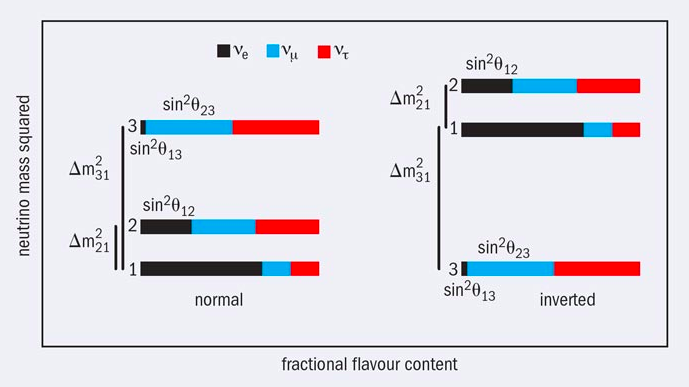
\includegraphics[scale=0.3]{graphics/hierarchy.png}
      \end{columns}
\end{frame}

\begin{frame}
  \frametitle{Statistical Issues}
  \begin{columns}
    \column{0.5\textwidth}
  \begin{itemize}
    \item Oscillation Parameters are typically measured via MLE using the underlying PMNS model and comparing it to observation
    \item However, experiments collect only a handful of statistics. $\mathcal{O}(10-100)$ over years of operation for the $\nu_{\mu} \rightarrow \nu_{e}$ channel
    \item Oscillation probabilities have complicated dependence on multiple parameters $\implies$ difficult to delineate
    \item Confidence Intervals are hard to find as Likelihood ratios don't satisfy asymptotic properties.
    \item Let's illustrate this with a toy experiment..
  \end{itemize}
    \column{0.5\textwidth}
    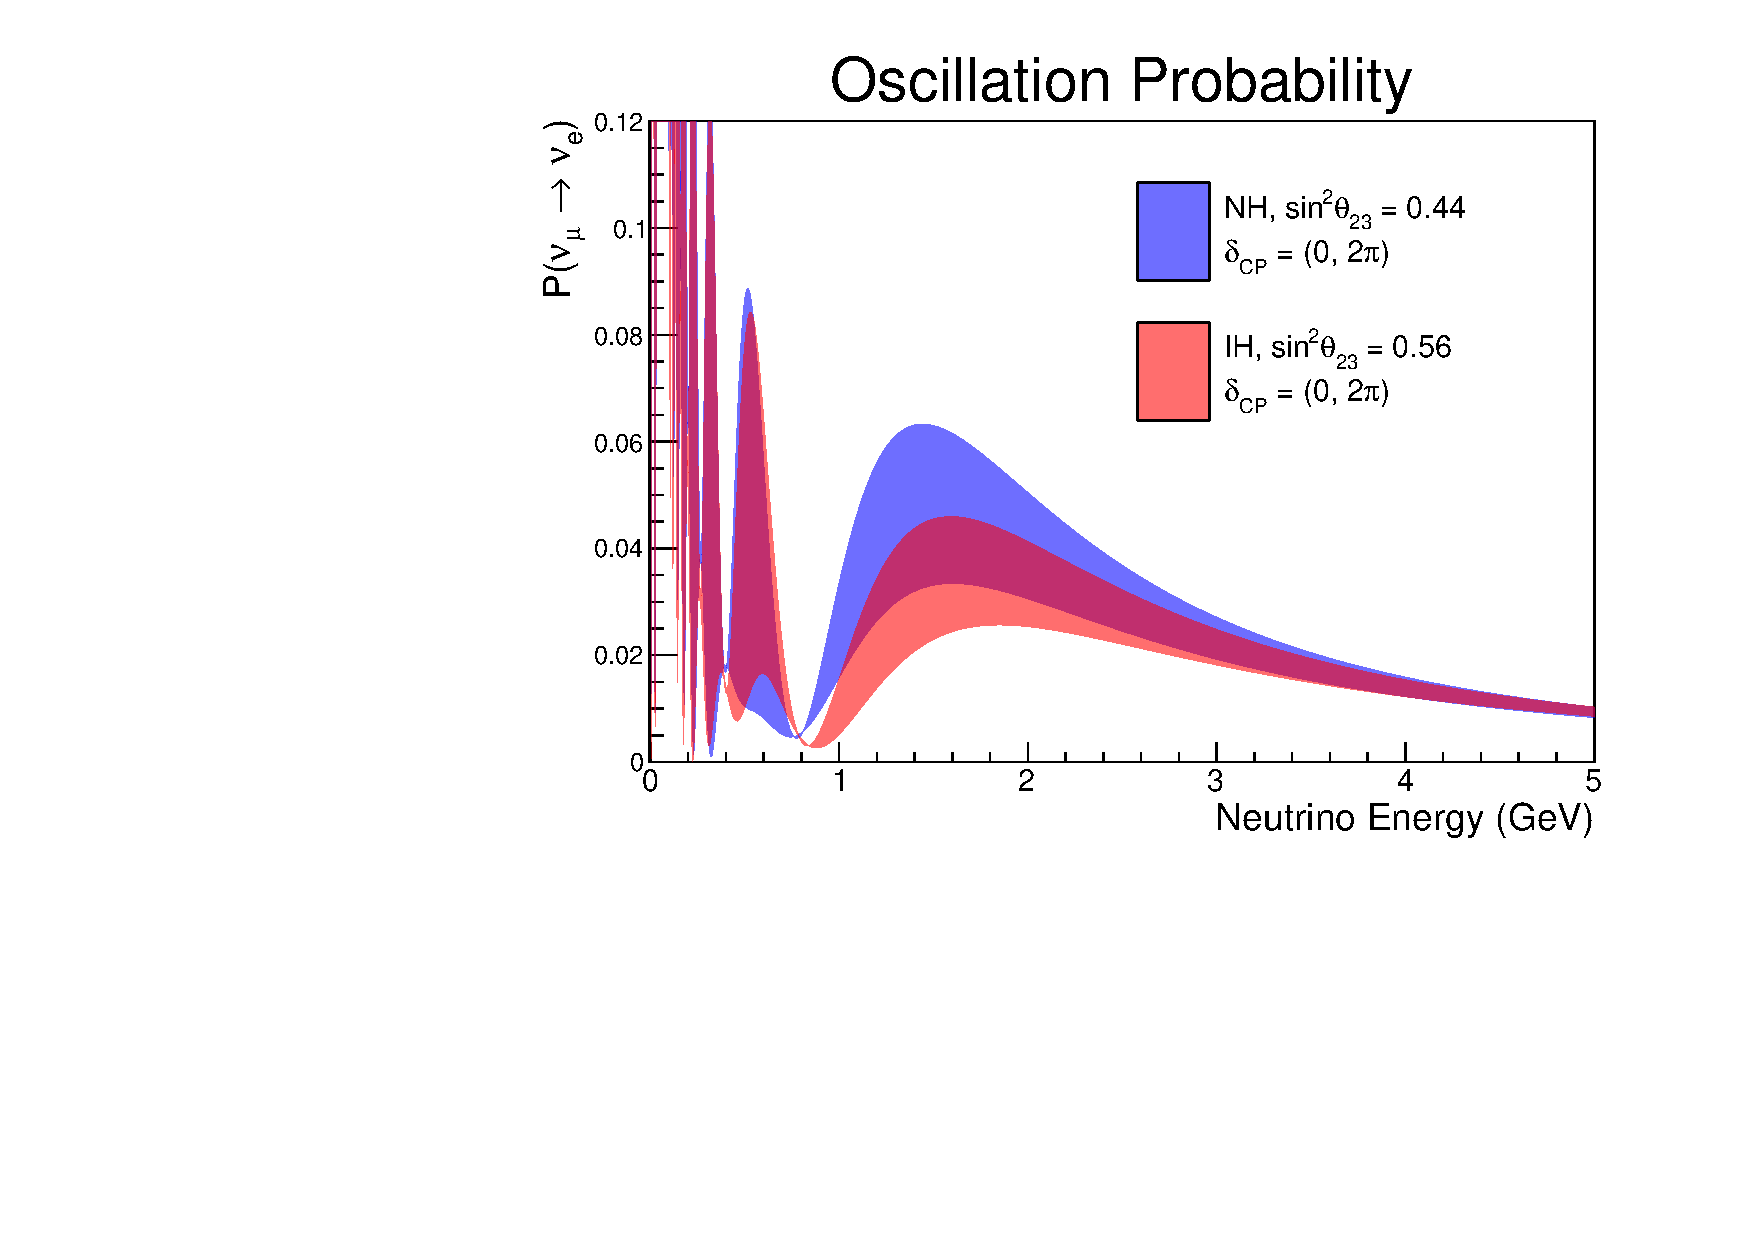
\includegraphics[scale=0.35]{figures_final/osc_shaded.pdf}
  \end{columns}
\end{frame}

\begin{frame}
  \frametitle{Toy Experiment}
  \begin{itemize}
    \item Modelled on NOvA. Baseline, $L = 810$km with $\nu_{\mu}$ flux peaking at $2$GeV
    \item $\nu_{\mu} \rightarrow \nu_{e}$ by multiplying toy shapes for flux, cross-section and oscillation probability.
    \item 10\% normalisation errors on flux and xsec model
  \end{itemize}
  \bigskip
  \begin{columns}
    \column{0.22\textwidth}
    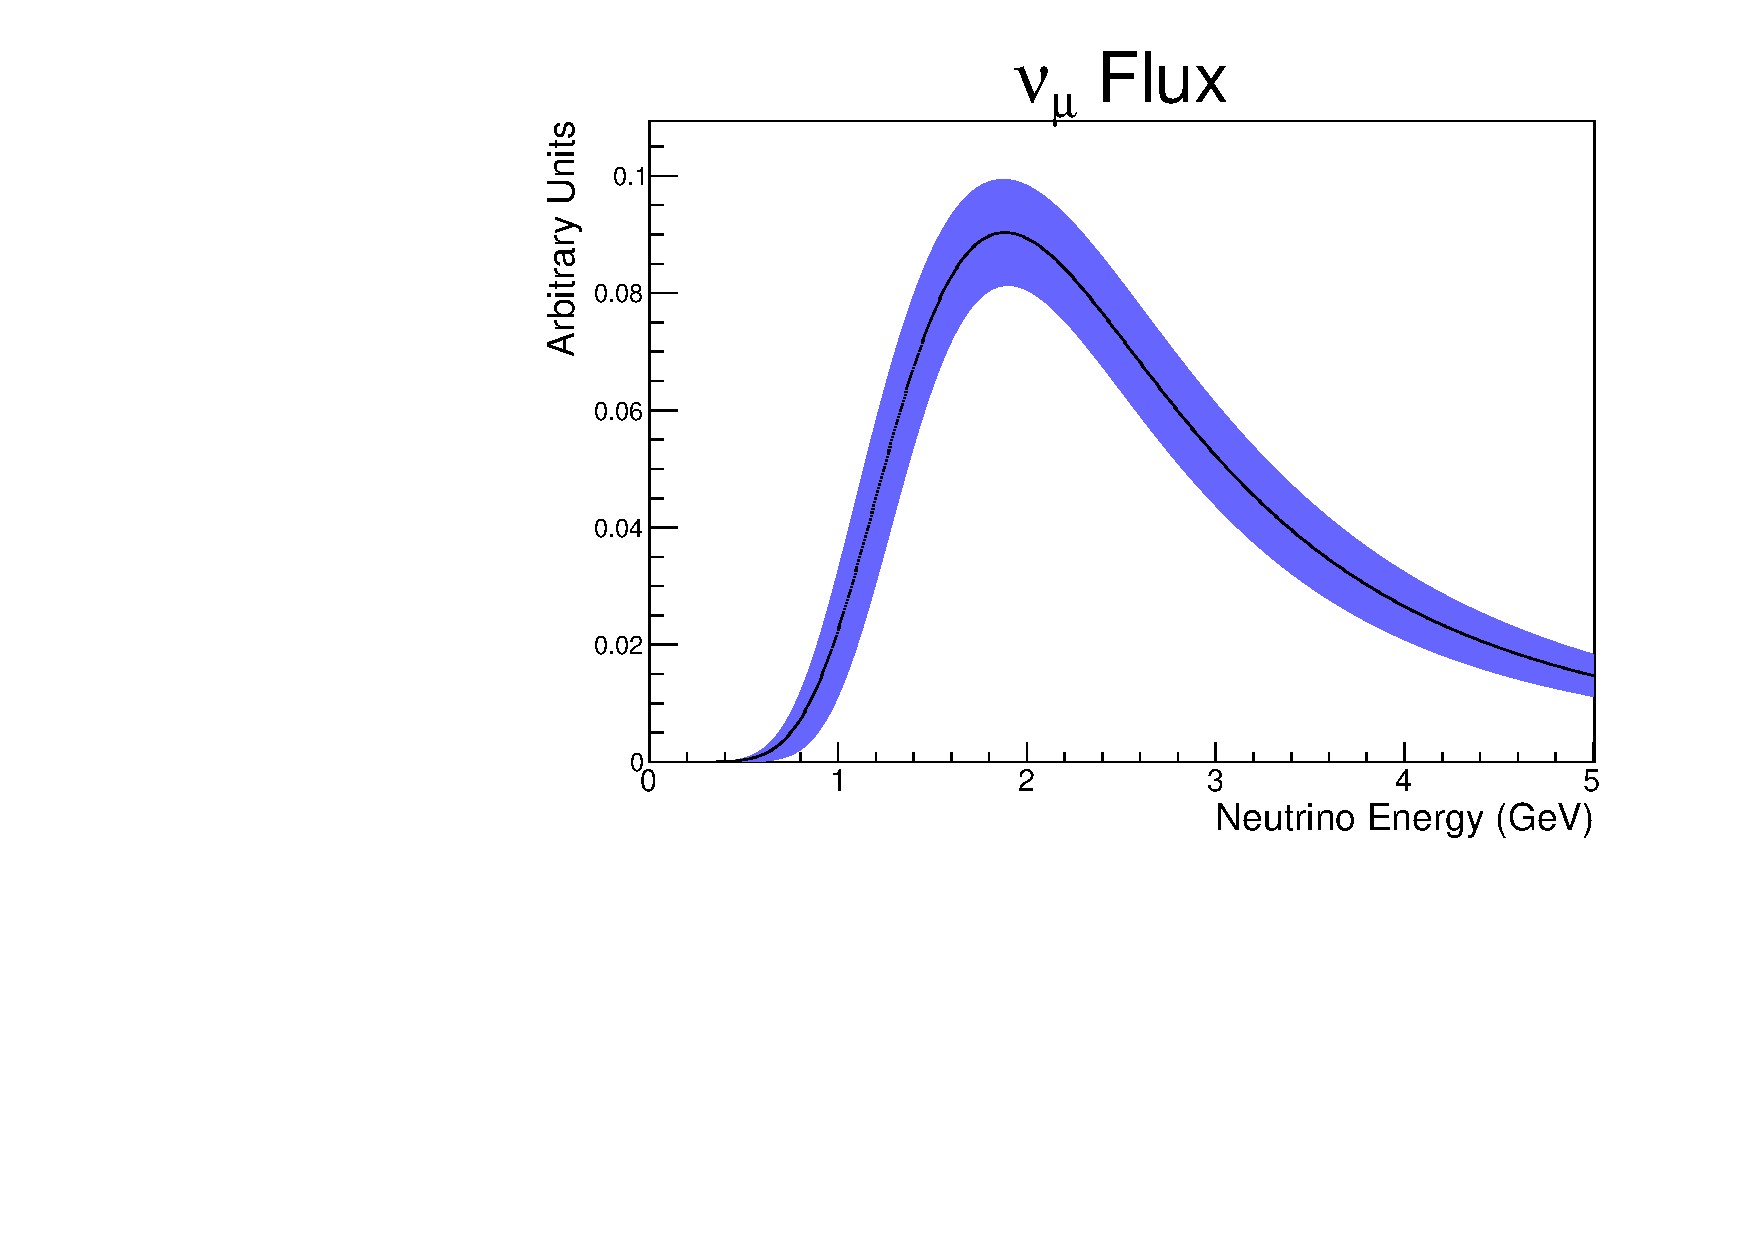
\includegraphics[scale=0.185]{figures_final/flux.pdf}
    \column{0.02\textwidth}
    \hfill *
    % \centering{*}
    \column{0.22\textwidth}
    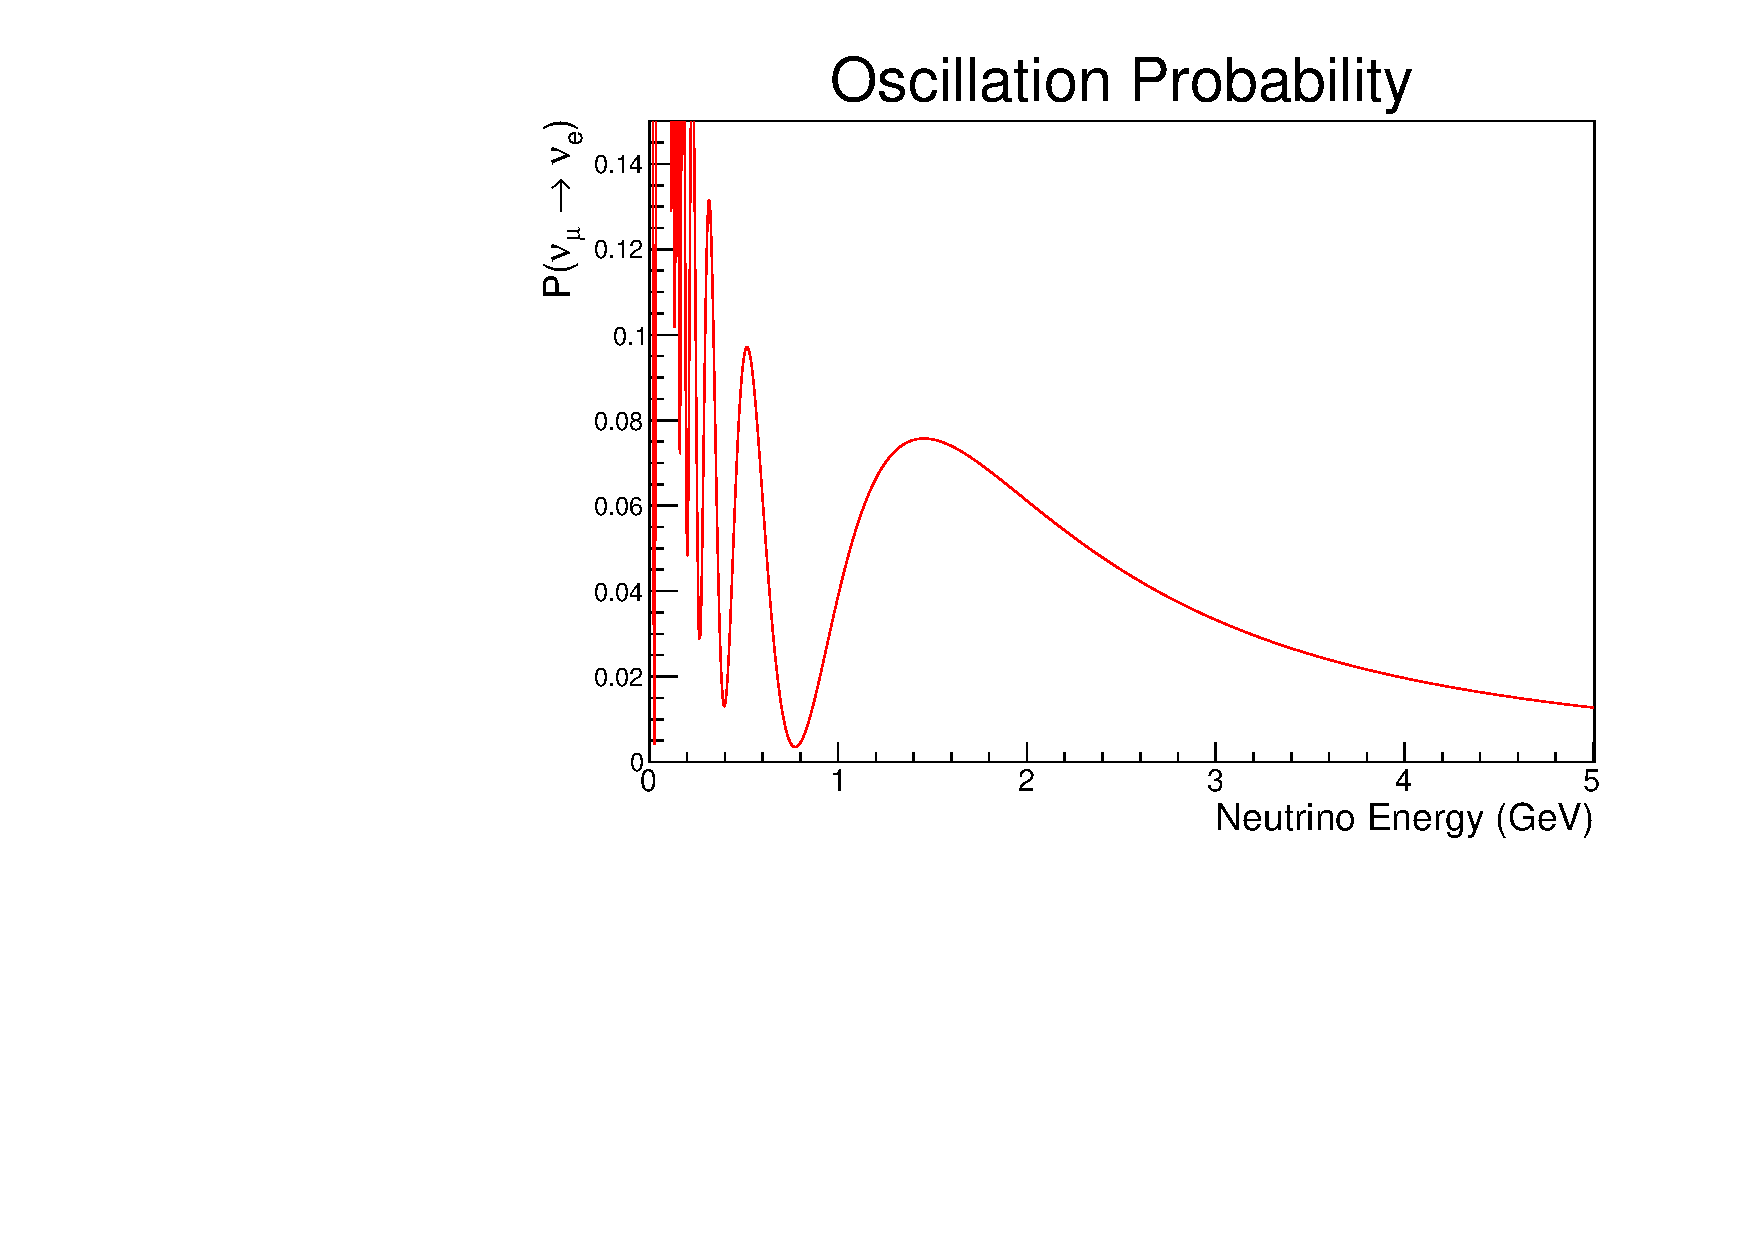
\includegraphics[scale=0.185]{figures_final/osc.pdf}
    \column{0.02\textwidth}
    \hfill *
    % \centering{*}
    \column{0.22\textwidth}
    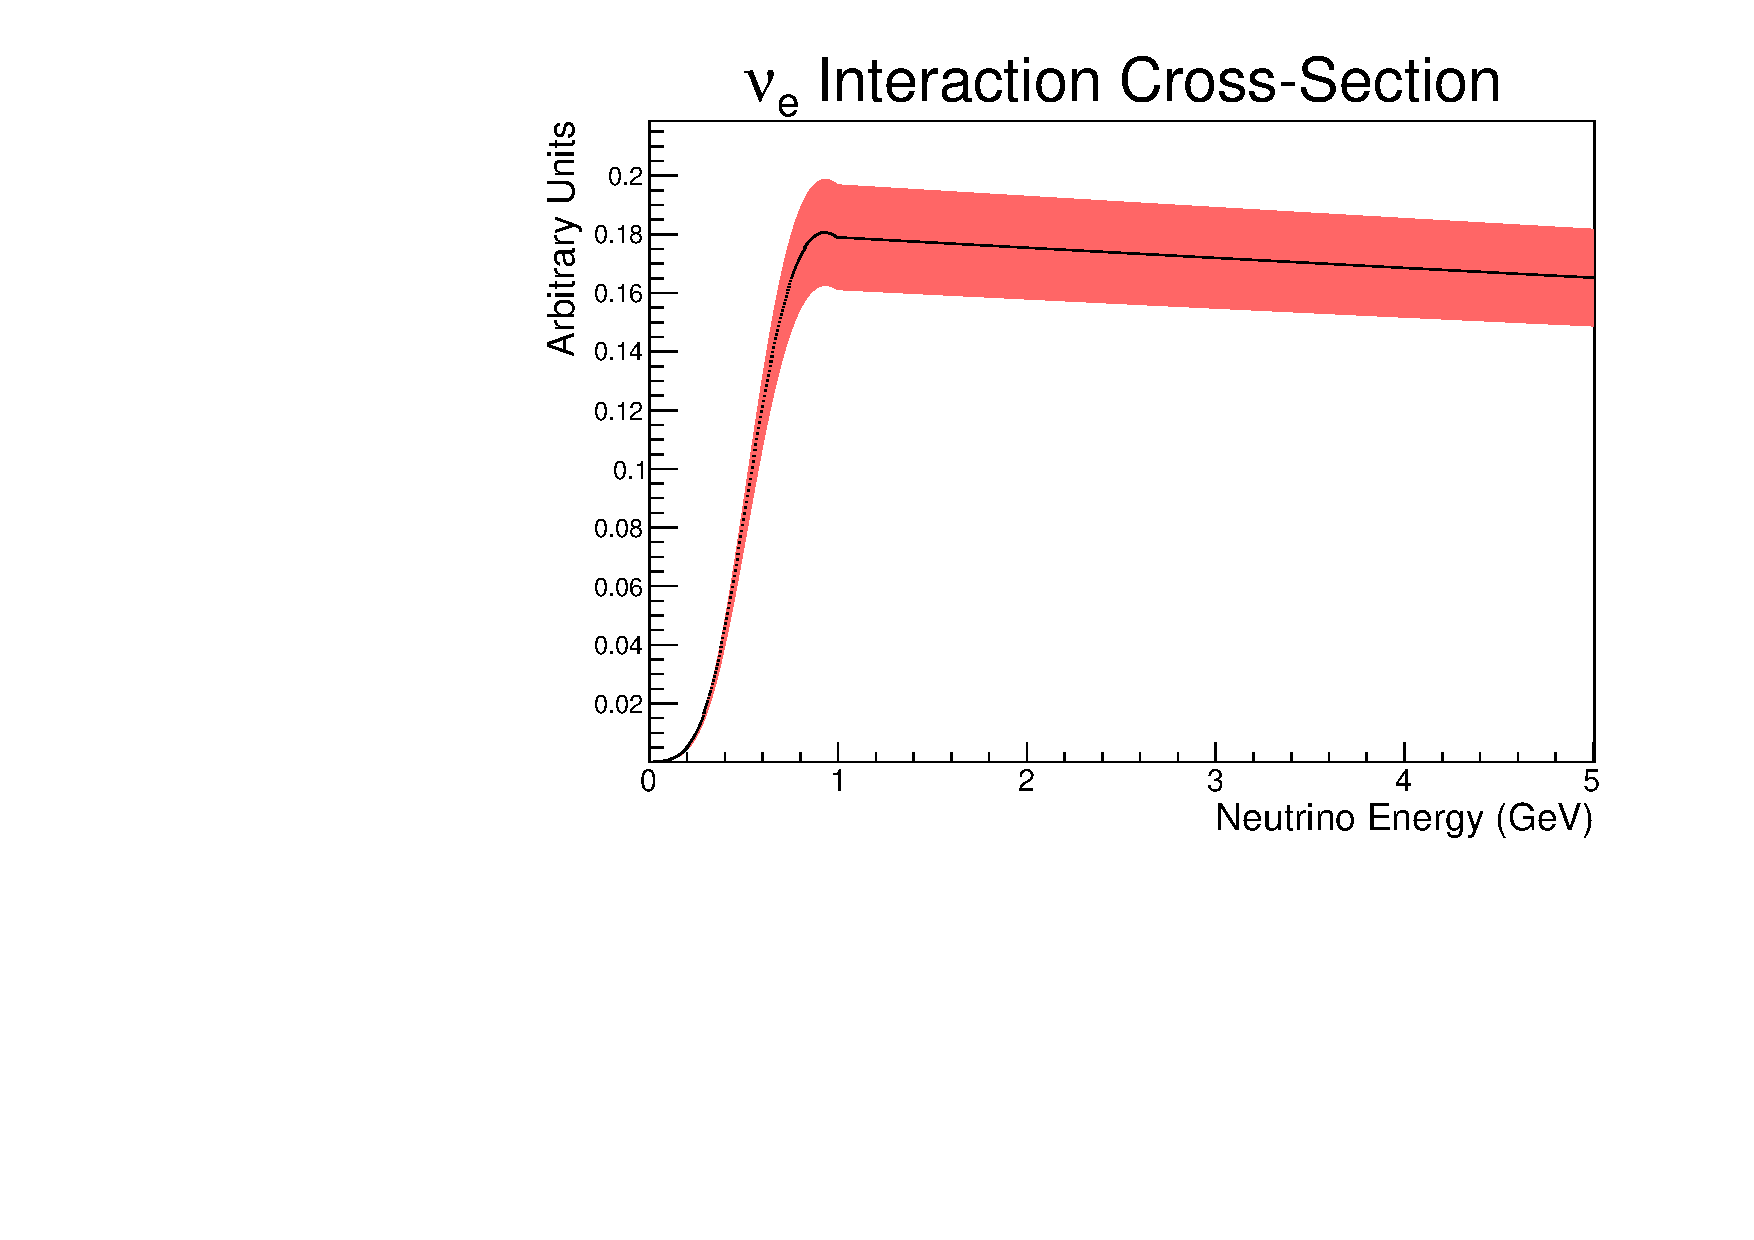
\includegraphics[scale=0.185]{figures_final/xsec.pdf}
    \column{0.03\textwidth}
    \hfill = 
    % \centering{=}
    \column{0.28\textwidth}
    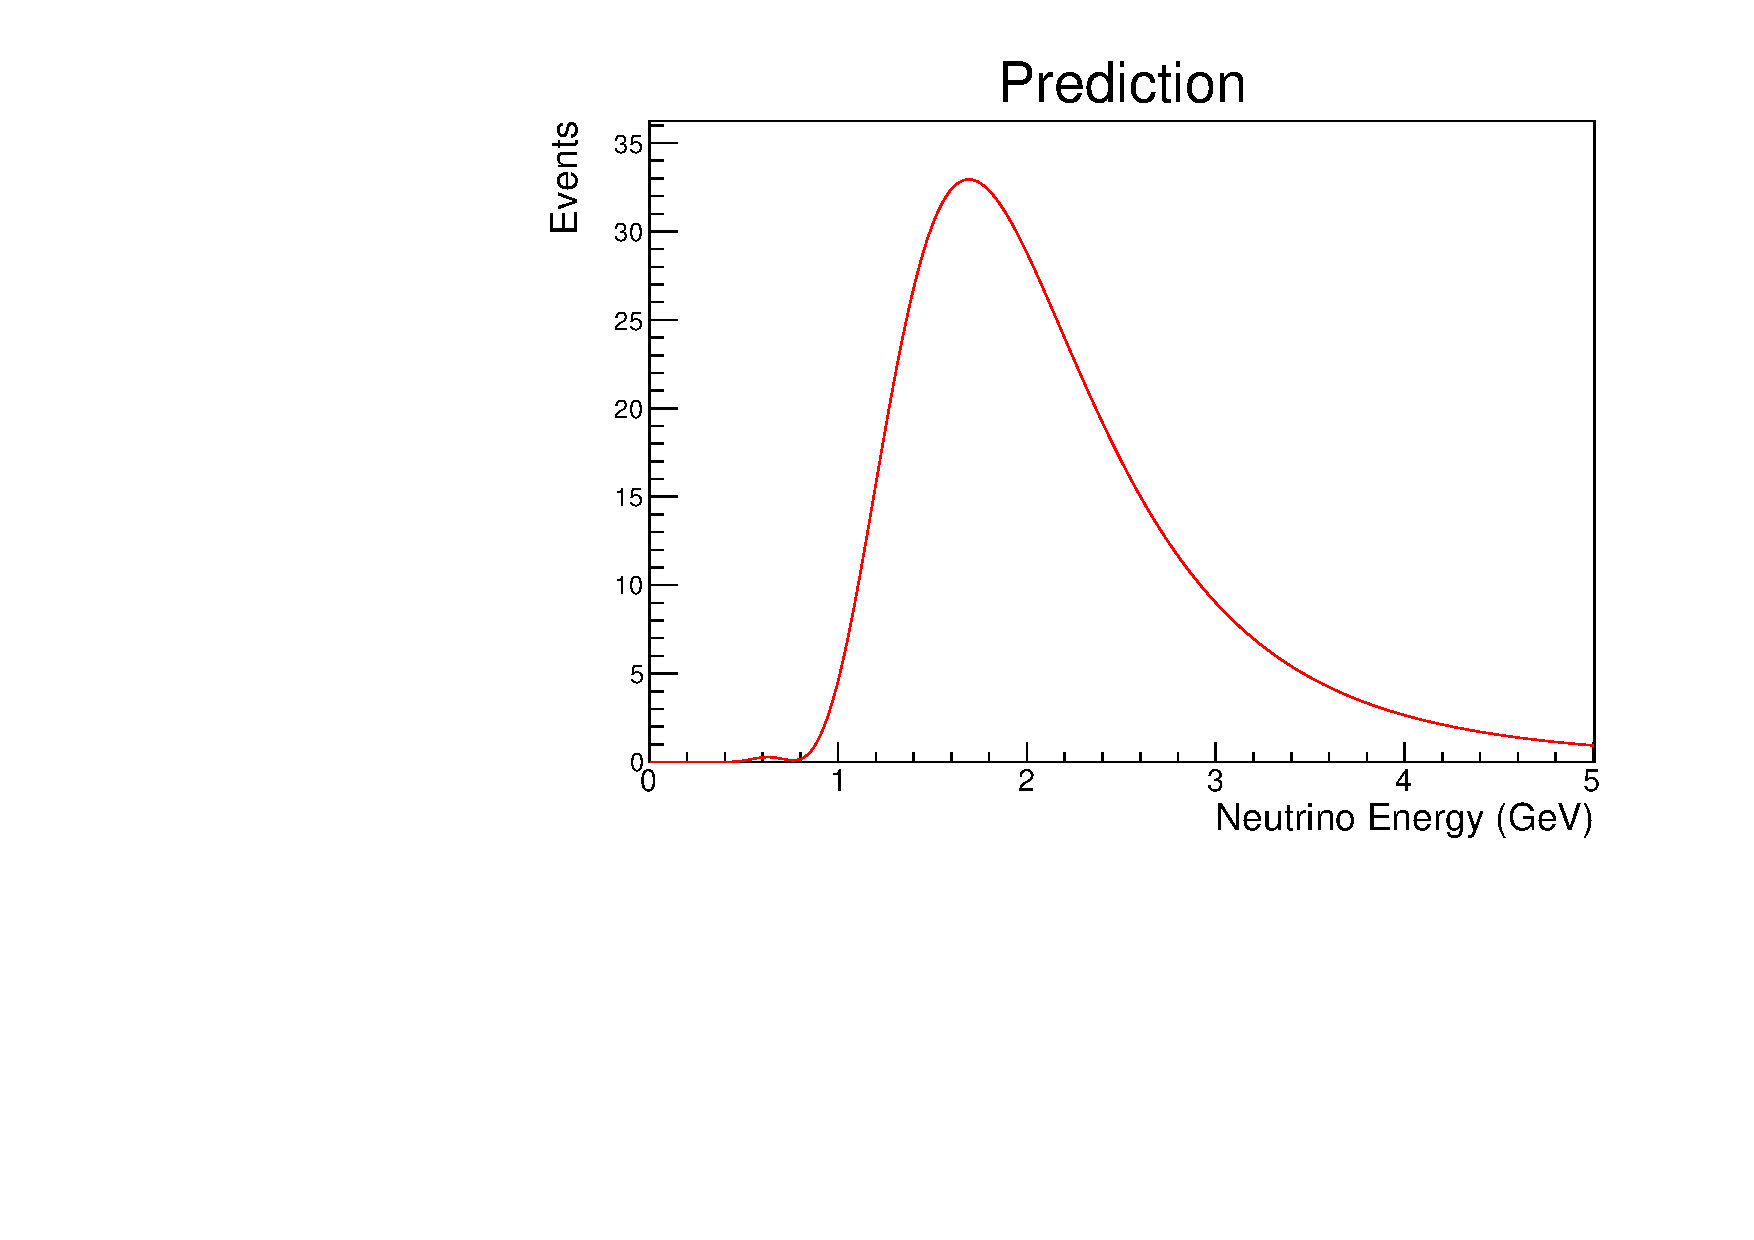
\includegraphics[scale=0.185]{figures_final/pred.pdf}
  \end{columns}
  \bigskip
  \begin{itemize}
    \item $P(\nu_{\mu} \rightarrow \nu_{e})$ using 3-flavor PMNS with MSW corrections added for matter propagation.
    \item Similar setup for $\nu_{\mu} \rightarrow \nu_{\mu}$ to constrain $sin^{2}(2\theta_{23})$ and $|\Delta m^2_{32}|$ but with 2-flavor approximation
    \item $P(\nu_{\mu} \rightarrow \nu_{\mu}) \sim 1 - sin^{2}(2\theta_{23})sin^{2}(\Delta m^2_{32}L/4E)$ 
  \end{itemize}
\end{frame}

\begin{frame}
  \frametitle{Toy Experiment}
  \begin{columns}
    \column{0.5\textwidth}
    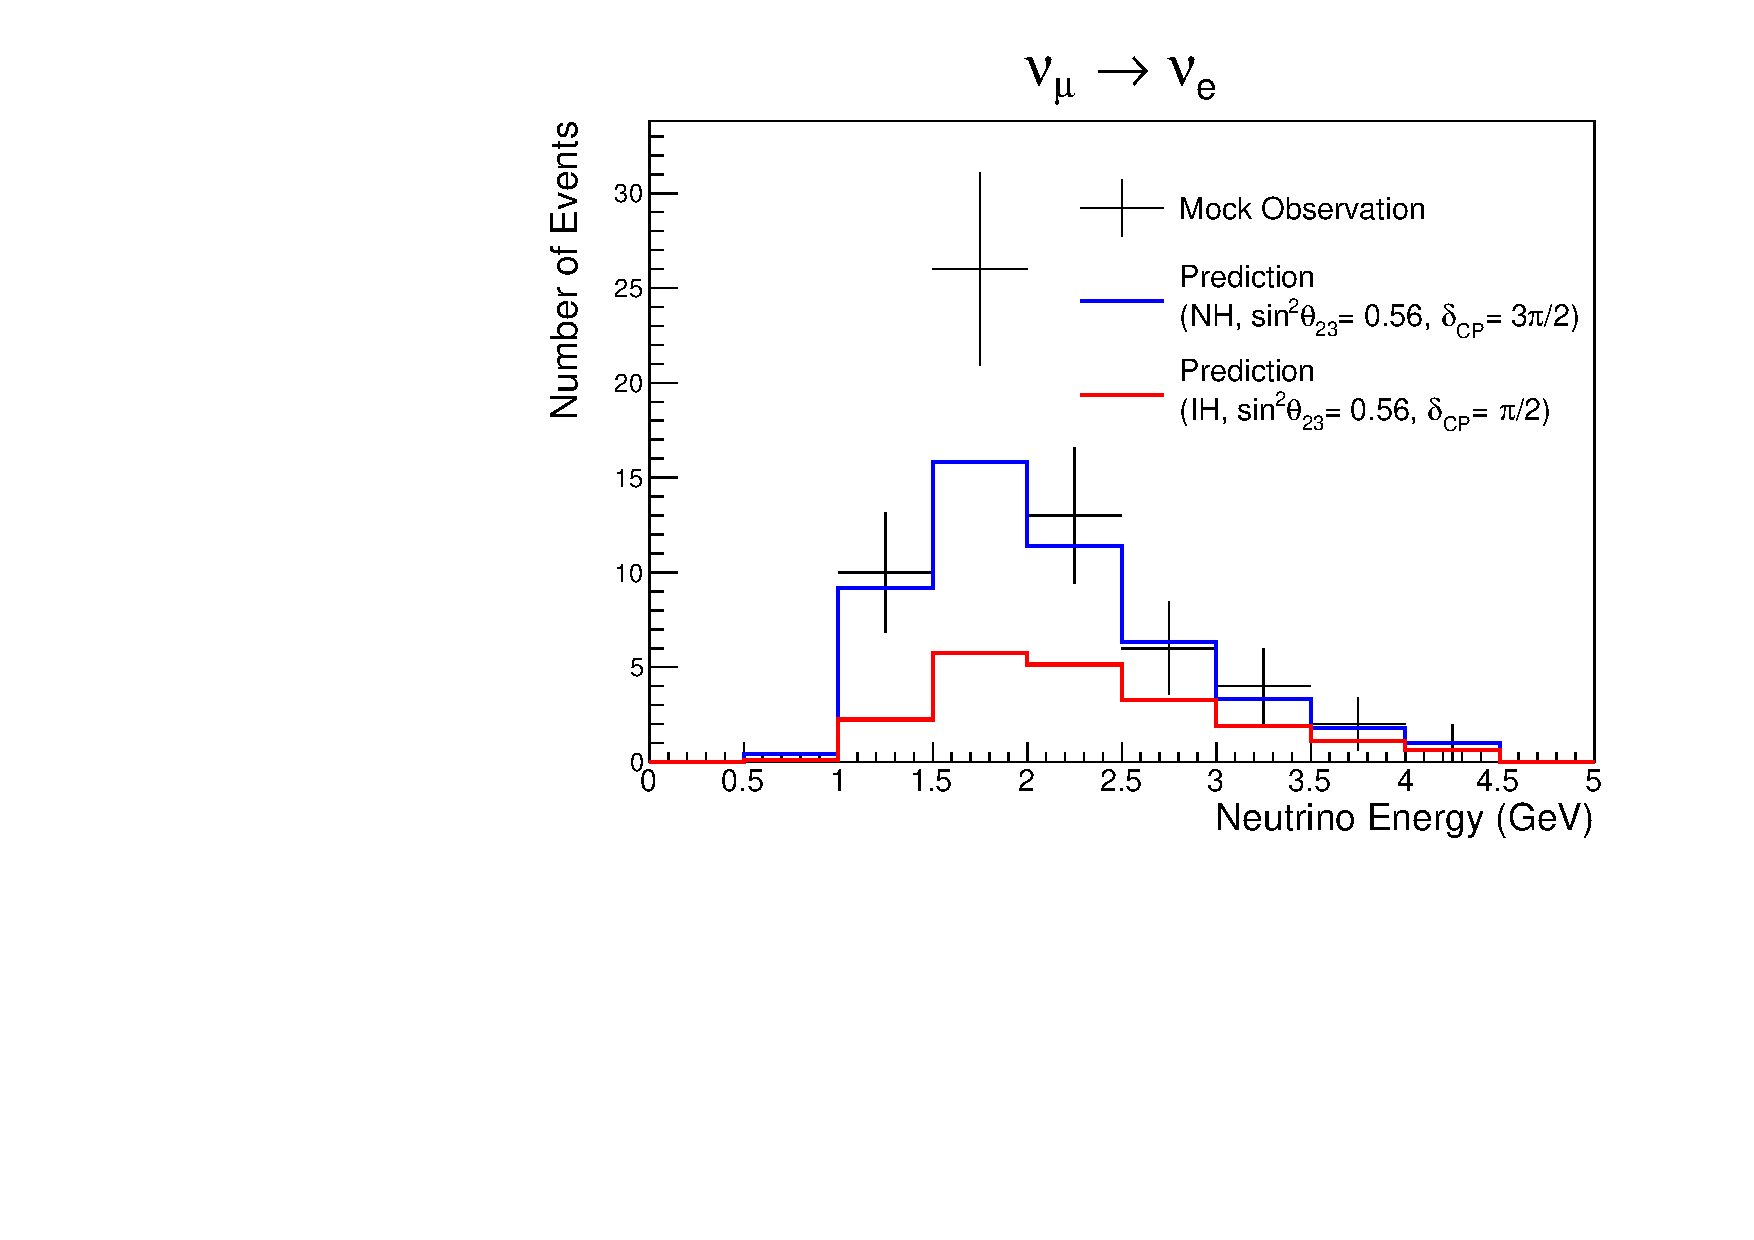
\includegraphics[scale=0.35]{figures_final/datamc_nue.pdf}
    \column{0.5\textwidth}
    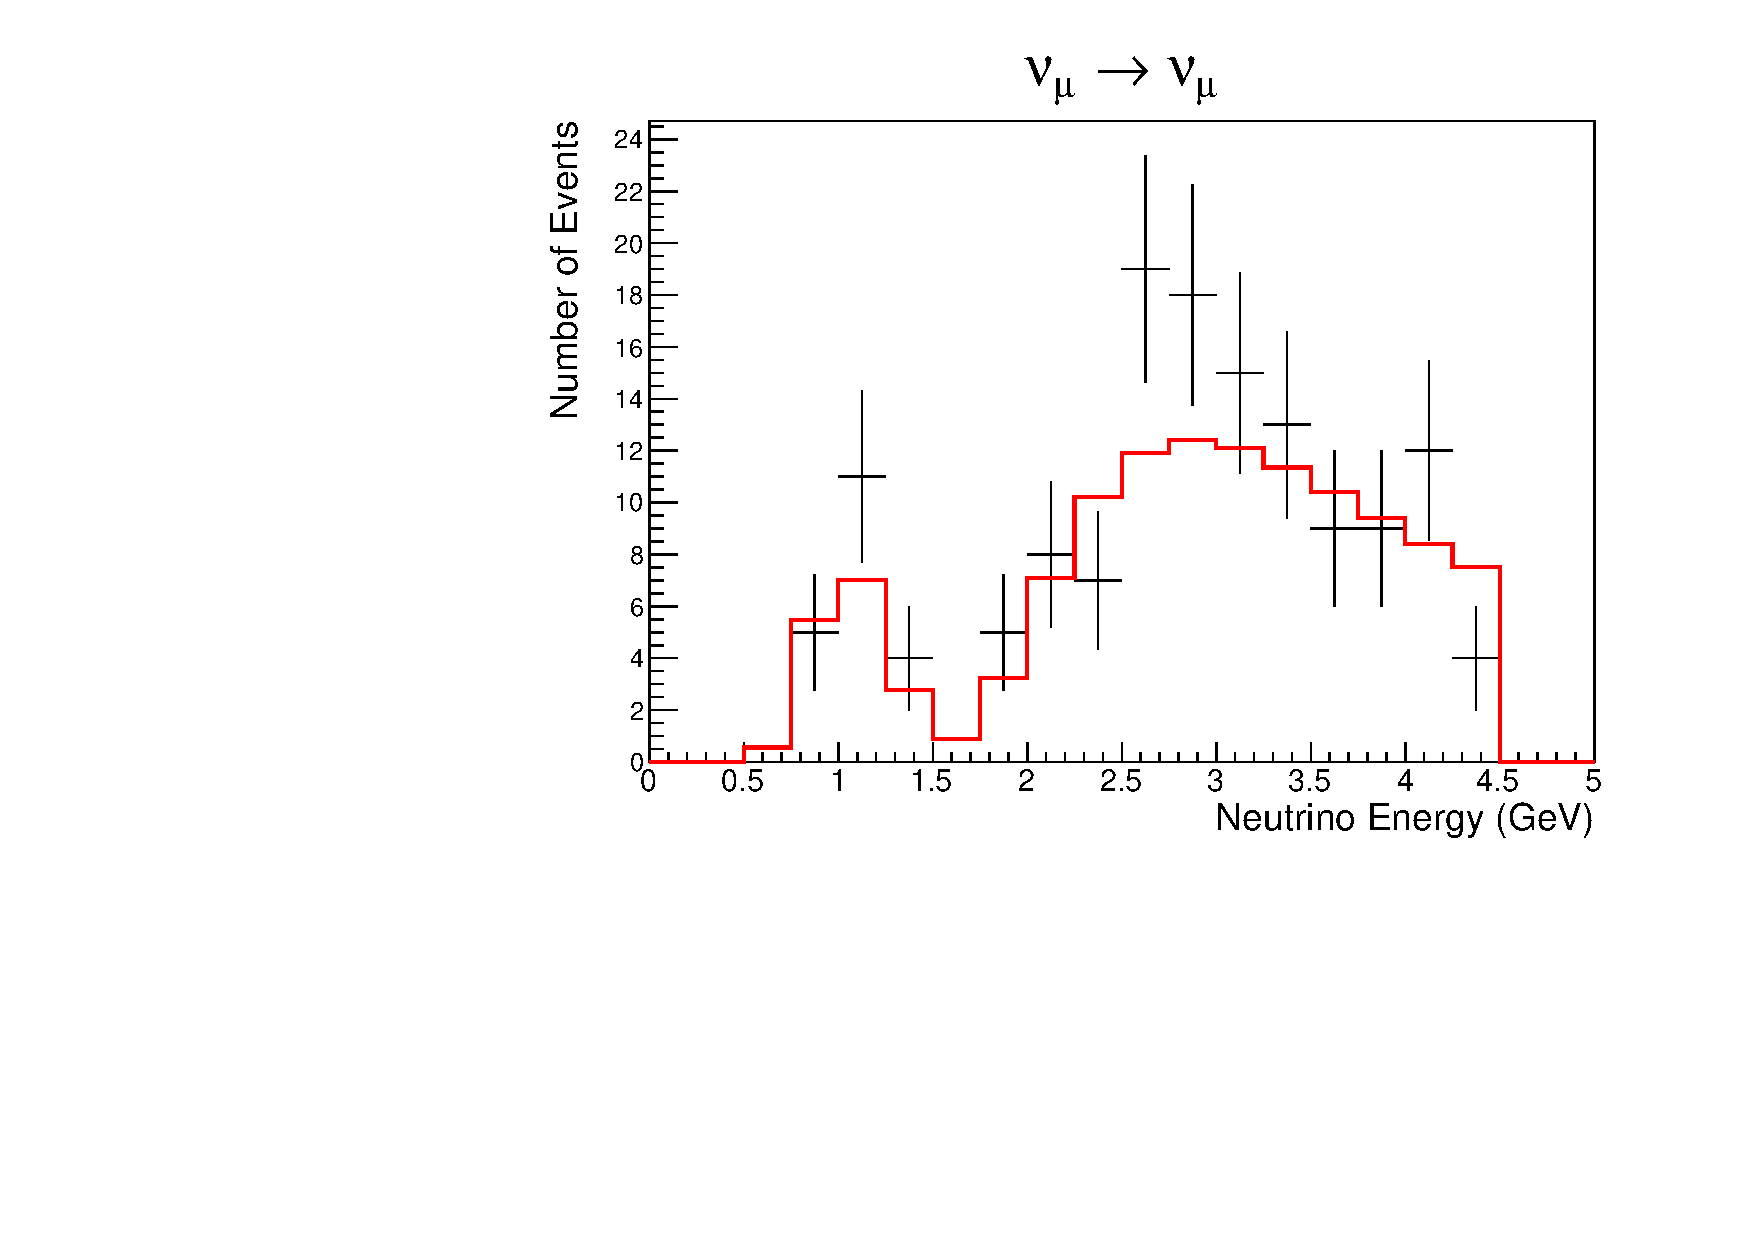
\includegraphics[scale=0.35]{figures_final/datamc_numu.pdf}
  \end{columns}
  \bigskip
  \begin{itemize}
    \item Toy data ($\vec{x}$) from Poisson variations at some chosen oscillation parameters.
    % \item $sin^{2}\theta_{23} = 0.56$, $\Delta m^2_{32} = 2.44\times10^{-3} eV^{2}$, $\delta_{CP} = 1.5\pi$
    \item With $(\theta, \delta)$ denoting list of oscillation and nuisance (flux and xsec errors) parameters, 
    \item Best-fit $(\hat{\theta}, \hat{\delta})$ found by minimizing negative log-likelihood over energy bins, $i$ 
      \begin{equation*}
        -2\log L(\theta, \delta) = -2\sum_{i\in I} \log Pois(x_i;v(\theta, \delta)_i) - \sum_{i \in I}x_i + \sum_{i \in I}v(\theta, \delta)_i +\delta^2
      \end{equation*}
    % \item where $v(\theta, \delta)$ is the expectation calculated through Monte-Carlo simulations.
    % \item Joint fit of $\nu_{\mu} \rightarrow \nu_{\mu}$ and $\nu_{\mu} \rightarrow \nu_{e}$ channels
      \end{itemize}
\end{frame}

\begin{frame}
  \frametitle{Confidence Intervals}
  \begin{itemize}
    \item $\theta_{0}$ included in the $1-\alpha$ confidence contour if we fail to reject the null ($\theta = \theta_{0}$) at $\alpha$ level
    \item Use an Inverted Likelihood Ratio Test (LRT)
    \item Neyman-Pearson Lemma : Likelihood Ratio (LR) is the most powerful test statistic
      \bigskip
      \begin{columns}
        \column{0.5\textwidth}
        \begin{figure}
        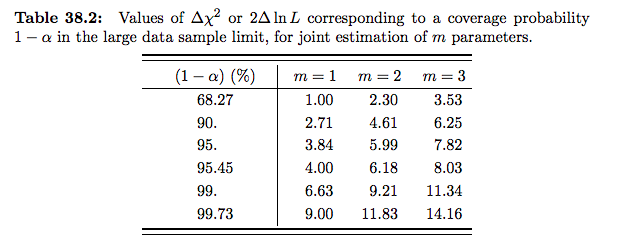
\includegraphics[scale=0.33]{graphics/wilks.png}
        \caption{From the PDG Review on Statistics}
        \end{figure}
        \column{0.5\textwidth}
        \begin{itemize}
    \item Easy to estimate in the asymptotic case as LR is a $\chi^{2}$ distribution. (Wilks Theorem)
    \item However, that's not the case here! 
    \item Proceed via Unified approach (Feldman-Cousins, 1998)
        \end{itemize}
      \end{columns}
  \end{itemize}
\end{frame}

\begin{frame}
  \frametitle{Feldman-Cousins}
  \begin{itemize}
    \item Seminal result giving an ordering principle for confidence intervals in non-asymptotic cases
    \item For given $\theta_{0}$, explicitly simulate distribution of test statistic, LR via Monte-Carlo experiments at $\theta_{0}$
    % \item Accept $\theta_{0}$ at say 68\% level if LR for observed data at $\theta_{0}$ is within 68\% of the distribution.
  \end{itemize}
  \begin{columns}
    \column{0.5\textwidth}
  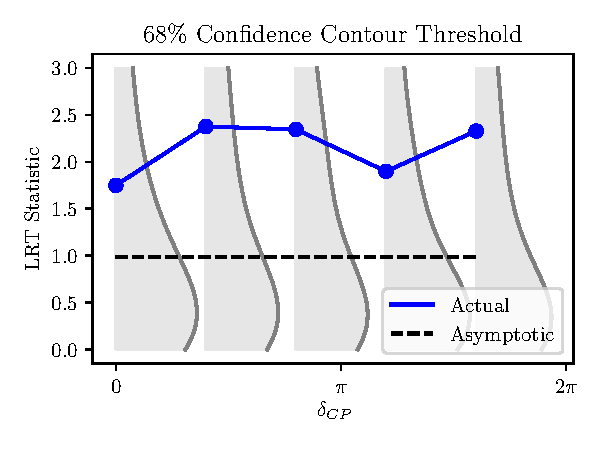
\includegraphics[scale=0.7]{figures_final/threshold.pdf}
    \column{0.5\textwidth}
  \begin{itemize}
    \item 68\% confidence interval for $\delta_{CP}$ : All $\delta_{CP}$ values for which LR for observed data (critical value) lies within threshold
    \item Confidence of rejecting given $\delta_{CP} = \delta_{0}$ given by percentile of $crit(\delta_{0})$
    \item Gives us the "correct" confidence interval in the frequentist sense by construction, since its essentially a grid search over the entire parameter space.
  \end{itemize}
  \end{columns}
\end{frame}

\begin{frame}
  \frametitle{A more efficient FC}
    \begin{itemize}
      \item Grid search across multi-dimensional parameter space $\implies$ extremely intense computational demands
      \item It'd be nice to be able to come up with a more refined search algorithm. 
        \bigskip
        \begin{columns}
          \column{0.5\textwidth}
          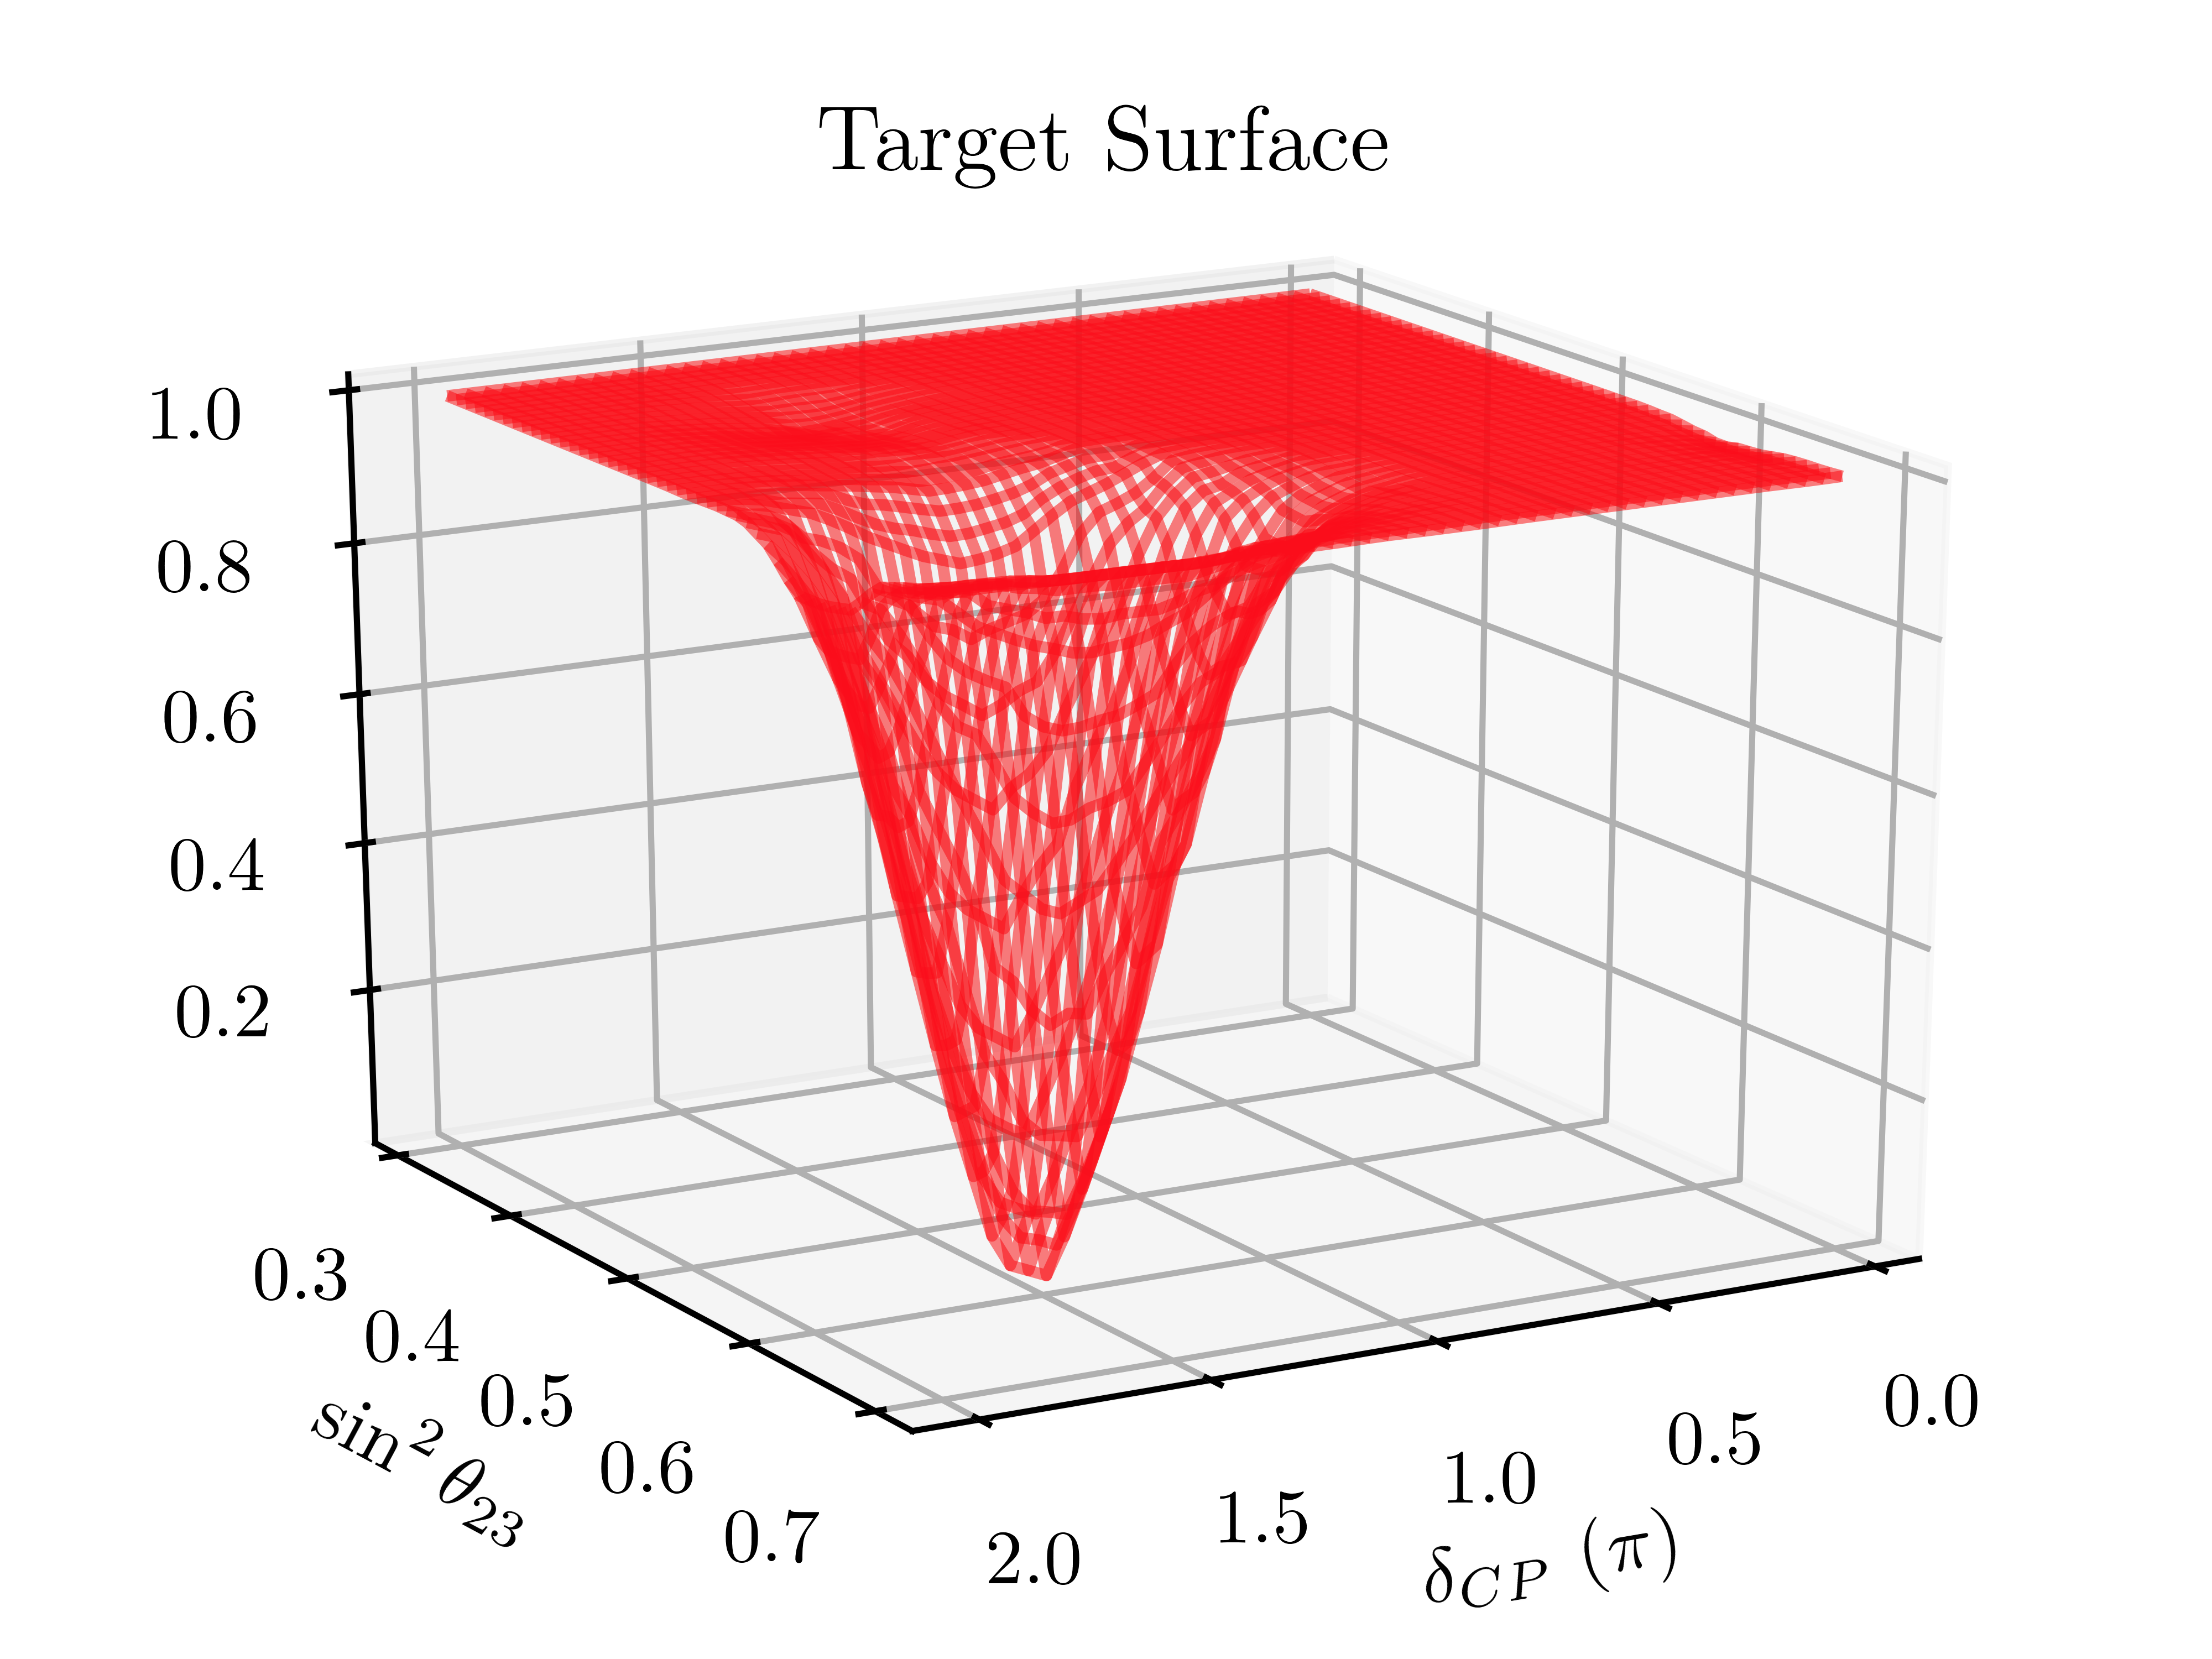
\includegraphics[scale=0.05]{figures_final/p_surface_ih.png}
          \column{0.5\textwidth}
      \item We can expect intuitively :
        \begin{itemize}
          \item Given a point in parameter space that is rejected at high confidence, it is likely that points near it will also be rejected
          \item Further, the variation in the LR percentiles ought to be smooth.
        \end{itemize}
      \item An efficient search would therefore : 
        \begin{itemize}
          \item Learn local features in the LR percentile surface to guide the search
          \item Favor simulating the LR test statistic distribution near the edge of the desired confidence contour than further out.
        \end{itemize}
        \end{columns}
    \end{itemize}
\end{frame}

\begin{frame}
  \frametitle{Bayesian Supervised Learning}
  \begin{itemize}
    \item Our goal is to approximate the FC percentile surface non parametrically using only a fraction of the grid points.
      \begin{columns}
        \column{0.5\textwidth}
    \item Classical supervised learning $\rightarrow$ training data to get best-fit model.  
    \item Predictions for new data are best-guess
    % \item If the true model is complicated and unknown apriori, need best-fit model with lots of parameters $\implies$ lots of training data.
      \column{0.5\textwidth}
    \item A Bayesian approach can assume a model itself to be a random variable with a certain probability distribution.
    \item Training data updates your priors about the model distribution
    \item Predictions for new data is a posterior distribution in model space. 
    \item Quantifies uncertainty in model estimates. Gets smaller with more training data
    \item Can be pretty non-parametric
      \end{columns}
  \end{itemize}
\end{frame}

\begin{frame}
  \frametitle{Gaussian Process}
  \begin{itemize}
    \item Special case of Bayesian Learning. Model distribution is an extension of multivariate gaussians to function space.
    \item Technically, its a probability measure defined over $\infty$-dim function space parameterized only by a mean function, $\mu(x)$ and a covariance function (kernel), $k(x, x')$
    \item We say, $f\sim\mathcal{GP}(\mu,k(\cdot,\cdot))$ if 
      \begin{equation*}
        \left(\begin{array}{c} f(x) \\ f(x') \end{array}\right)\sim\mathcal{N}(\left[\begin{array}{c} \mu(x) \\ \mu(x') \end{array}\right], \left[\begin{array}{c c} k(x,x) & k(x,x') \\ k(x,x') & k(x',x') \end{array}\right]).
      \end{equation*}
    \item Intuitively, we can picture each draw from a $\mathcal{GP}(\mu,k(\cdot,\cdot))$ giving us a different $f(x)$ with the average result being $\mu(x)$
    \item The kernel encodes the correlation between nearby points. A commonly used kernel is the radial basis function, $k(x,x')=\exp(-(x-x')^2/l^2)$
    \item A RBF kernel tells us that $\mathcal{GP}$ results at nearby points are highly influenced by observations at a given point while further out, they aren't. 
  \end{itemize}
\end{frame}

\begin{frame}
  \frametitle{Why $\mathcal{GP}$s?}
  \begin{itemize}
      \begin{columns}
        \column{0.5\textwidth}
    \item Enormously flexible! Can basically approximate any well behaved function with an appropriate choice of the kernel. 
    \item Predictions at new data points are computationally tractable with basic linear algebra, i.e for $\mathcal{GP}(\textbf{0},k(\cdot,\cdot))$ :
      \begin{equation*}
        f(x')|f(x)\sim \mathcal{N}(\frac{k(x,x')}{k(x,x)}f(x), k(x',x')-\frac{k(x,x')^2}{k(x,x)})
    \end{equation*}
        \column{0.5\textwidth}
      \centering{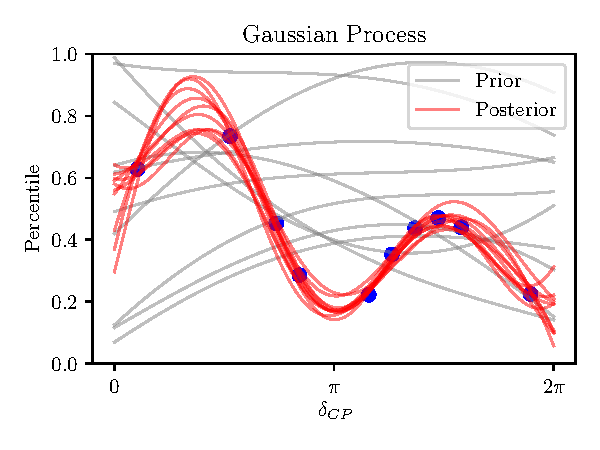
\includegraphics[scale=0.65]{figures_final/gp.pdf}}
      \end{columns}
    \item Kernel hyperparameters can be learned via maximising the likelihood of current set of observations marginalised over the function distribution, $f$
  \end{itemize}
\end{frame}
  
\begin{frame}
        \frametitle{$\mathcal{GP}$s in Literature}
        \begin{itemize}
  \item $\mathcal{GP}$s in HEP : arXiv:1709.05681, M.~Frate, K.~Cranmer et al. Using $\mathcal{GP}$s to describe background spectra in dijet resonance searches at the LHC non-parametrically.
  \item Used in Astrophysics for modelling stochasticity of light yields in stars, active galactic nuclei etc
  \item Many other fields! 
  \end{itemize}
\end{frame}

\begin{frame}
  \frametitle{$\mathcal{GP}$s for FC}
  \begin{itemize}
    \item Fitting a GP to target percentile surface for a given contour. (Stochasticity of the target surface) 
    \item "Observation" at a given point in parameter space, $\theta$ means simulating the LRT distribution and finding the percentile of $crit(\theta)$
    \item Choose a RBF Kernel with an additional term incorporating variance of percentile estimate at $\theta$. 
      \bigskip
      \begin{columns}
      \column{0.5\textwidth}
        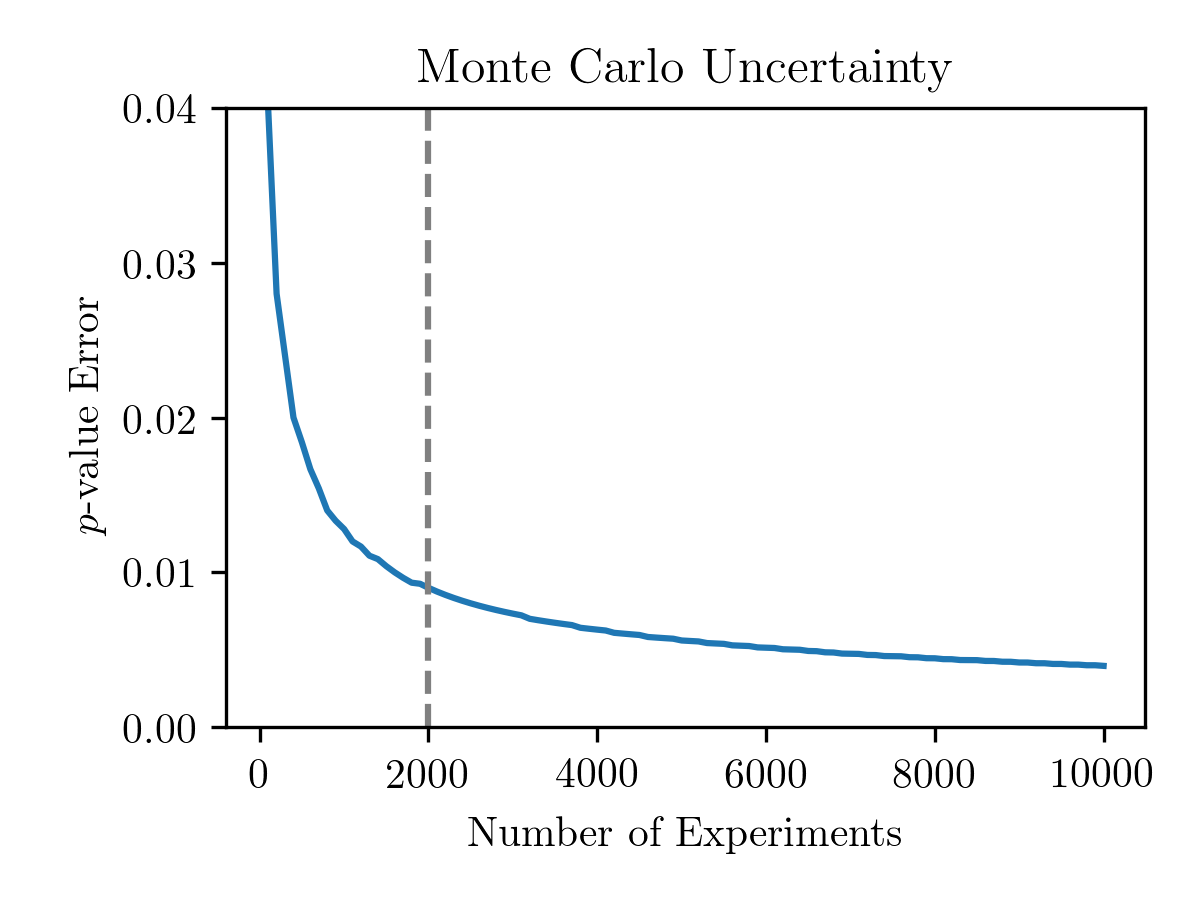
\includegraphics[scale=0.6]{figures_final/uncertainty.png}
        \column{0.5\textwidth}
      \item $k(\cdot, \cdot) = k_{RBF}(\cdot, \cdot) + \sigma_{p}^{2}I$
    \item The additional variance encodes the binomial error resulting from throwing finite number of experiments to simulate the LRT distribution at $\theta$
    \item Allows us to incorporate varying number of experiments thrown into the CI search, reducing computational burden further.  
      \end{columns}
  \end{itemize}
\end{frame}

\begin{frame}
  \frametitle{Optimised Confidence Interval Search}
  \begin{itemize}
    \item Use an acquisition function that proposes new points in $\theta$-space to explore based on $\mathcal{GP}$ approximated percentile surface.
      \begin{equation*}
    a(\theta) = \sum_{\alpha_i}|\frac{\hat{q}(\theta)-\alpha_i}{\sigma_{\hat{q}(\theta)}}|^{-1}
      \end{equation*}
    \item Here, $\hat{q}(\theta)$ is $\mathcal{GP}$ mean, $\sigma_{\hat{q}(\theta)}$ is $\mathcal{GP}$ std-dev, $\alpha_i$ is chosen to be $(0.68, 0.90)$
    \item $a(\theta)$ balances between exploration, i.e MC experiments at new points and exploitation, i.e reducing $\mathcal{GP}$ error
  \end{itemize}
  \begin{columns}
    \column{0.5\textwidth}
    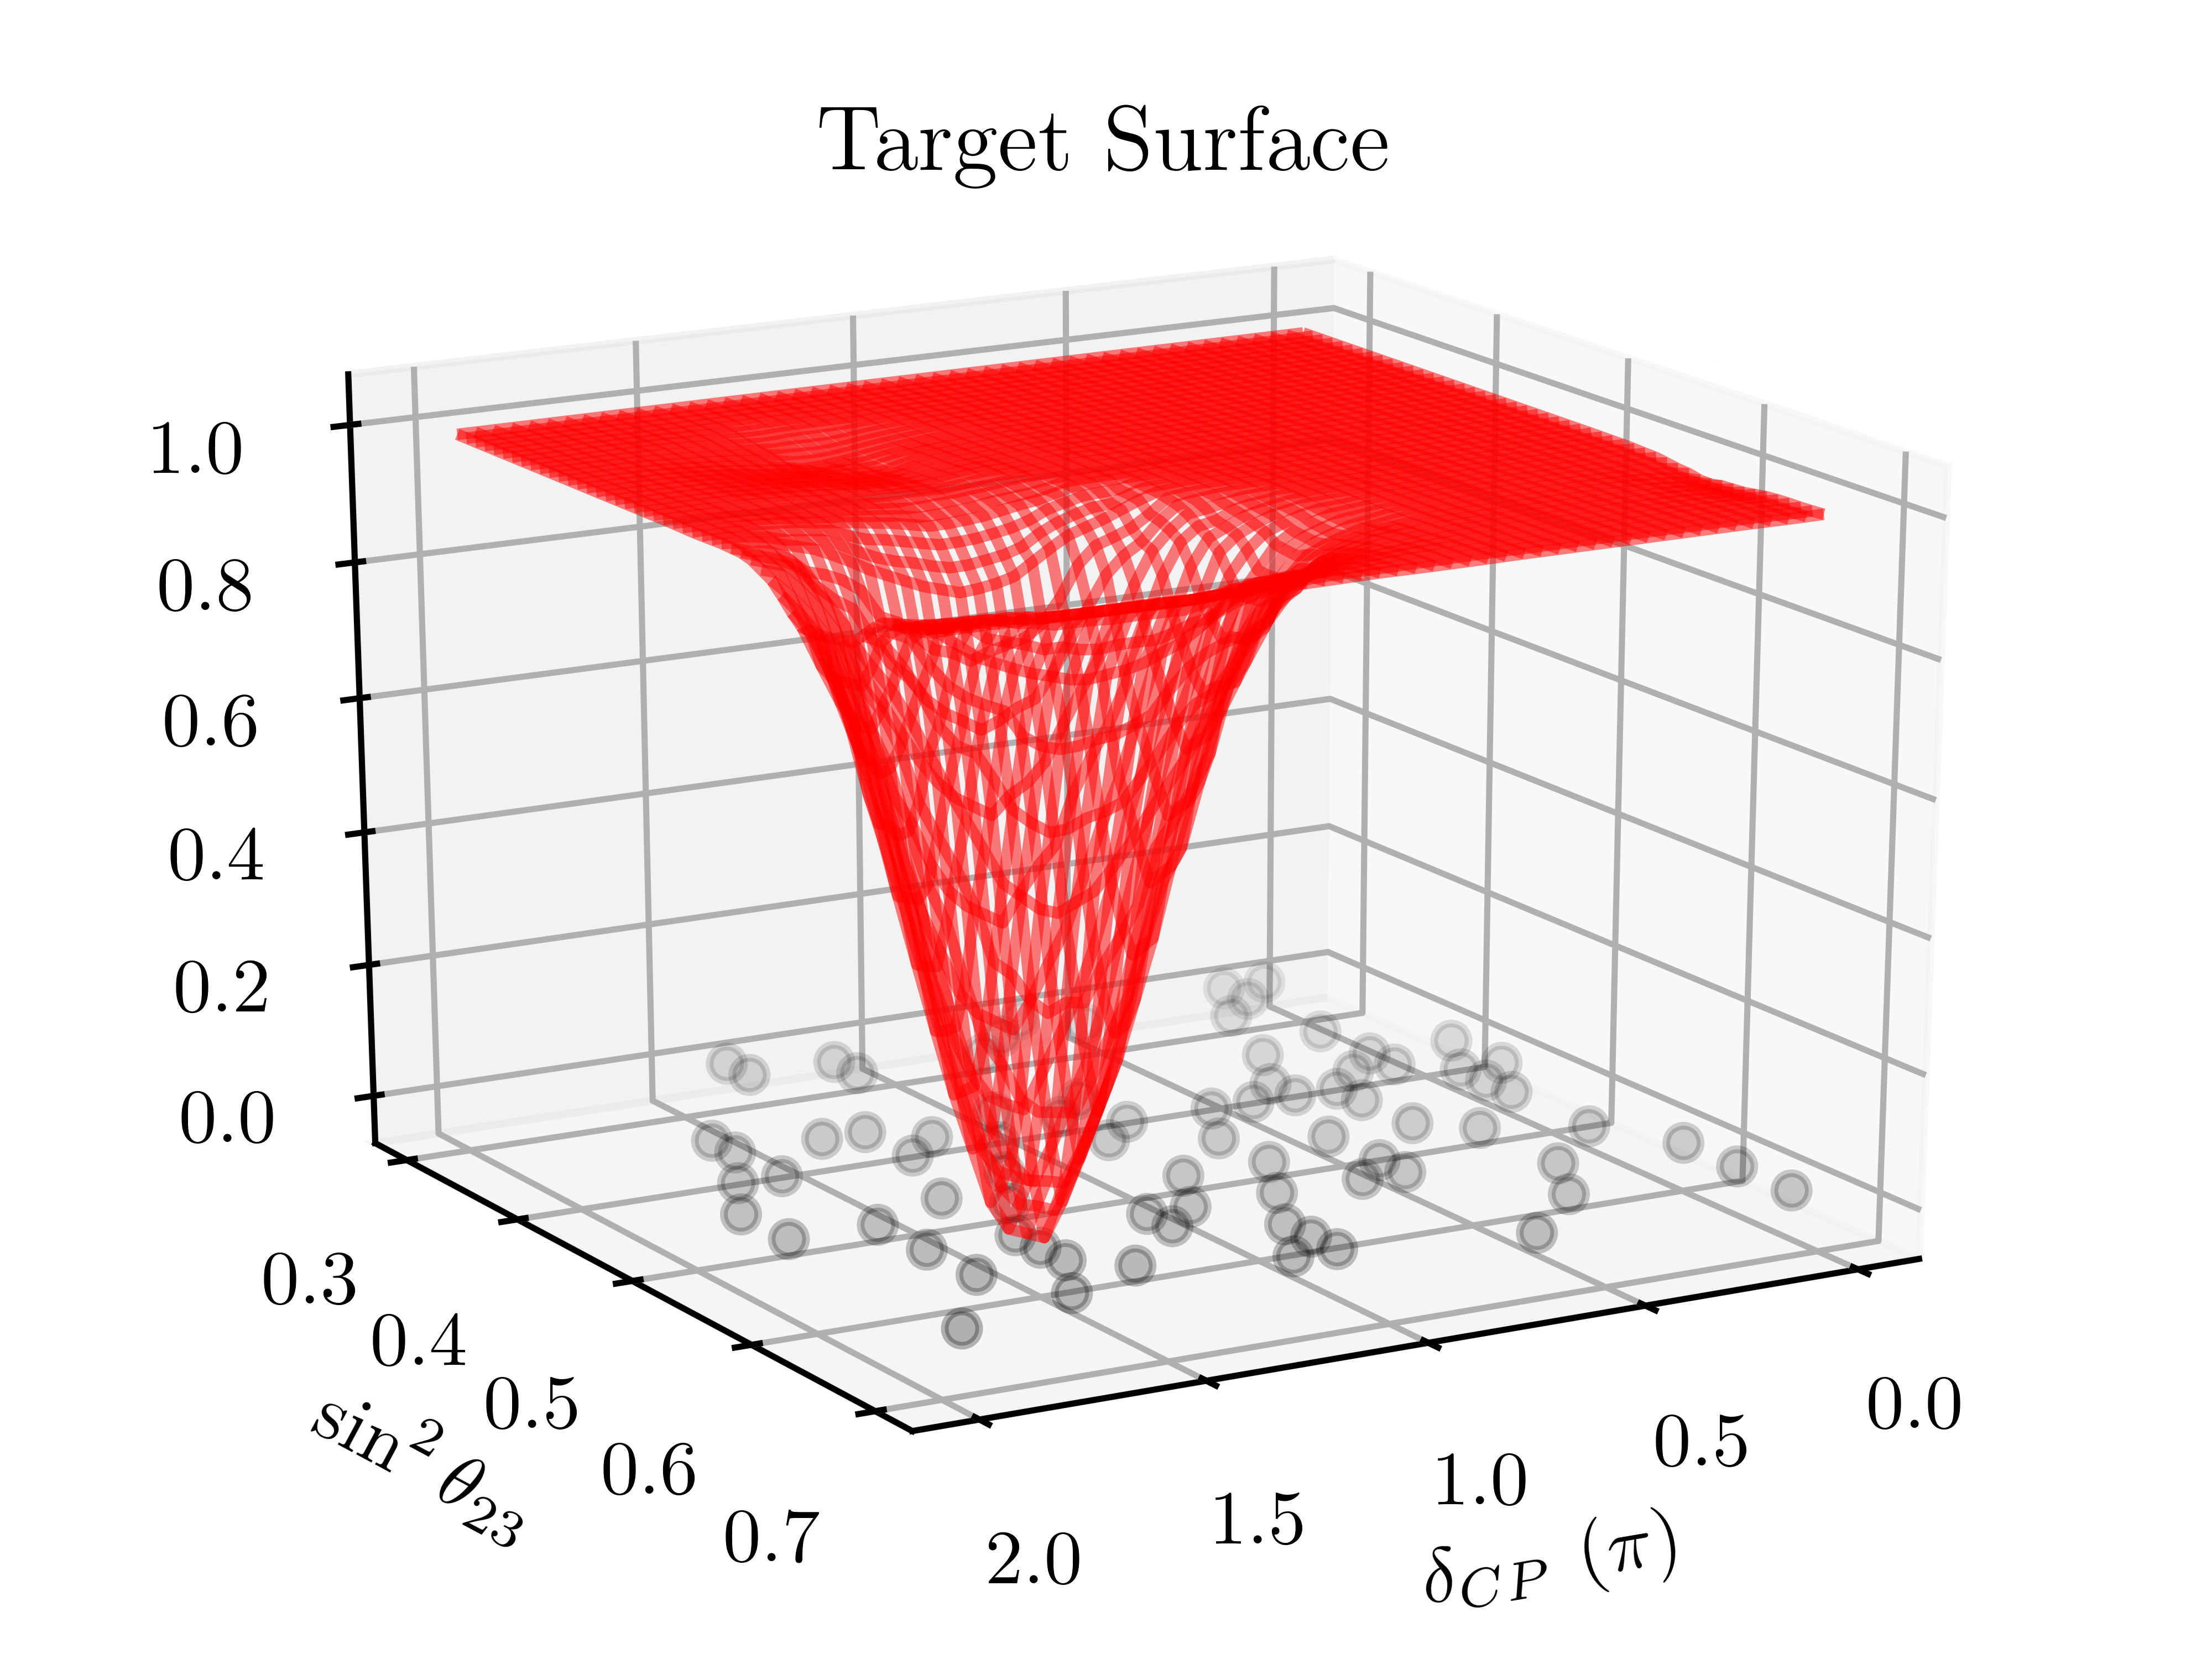
\includegraphics[scale=0.6]{figures_final/surface_sdcp_inverted_start.png}
    \column{0.5\textwidth}
    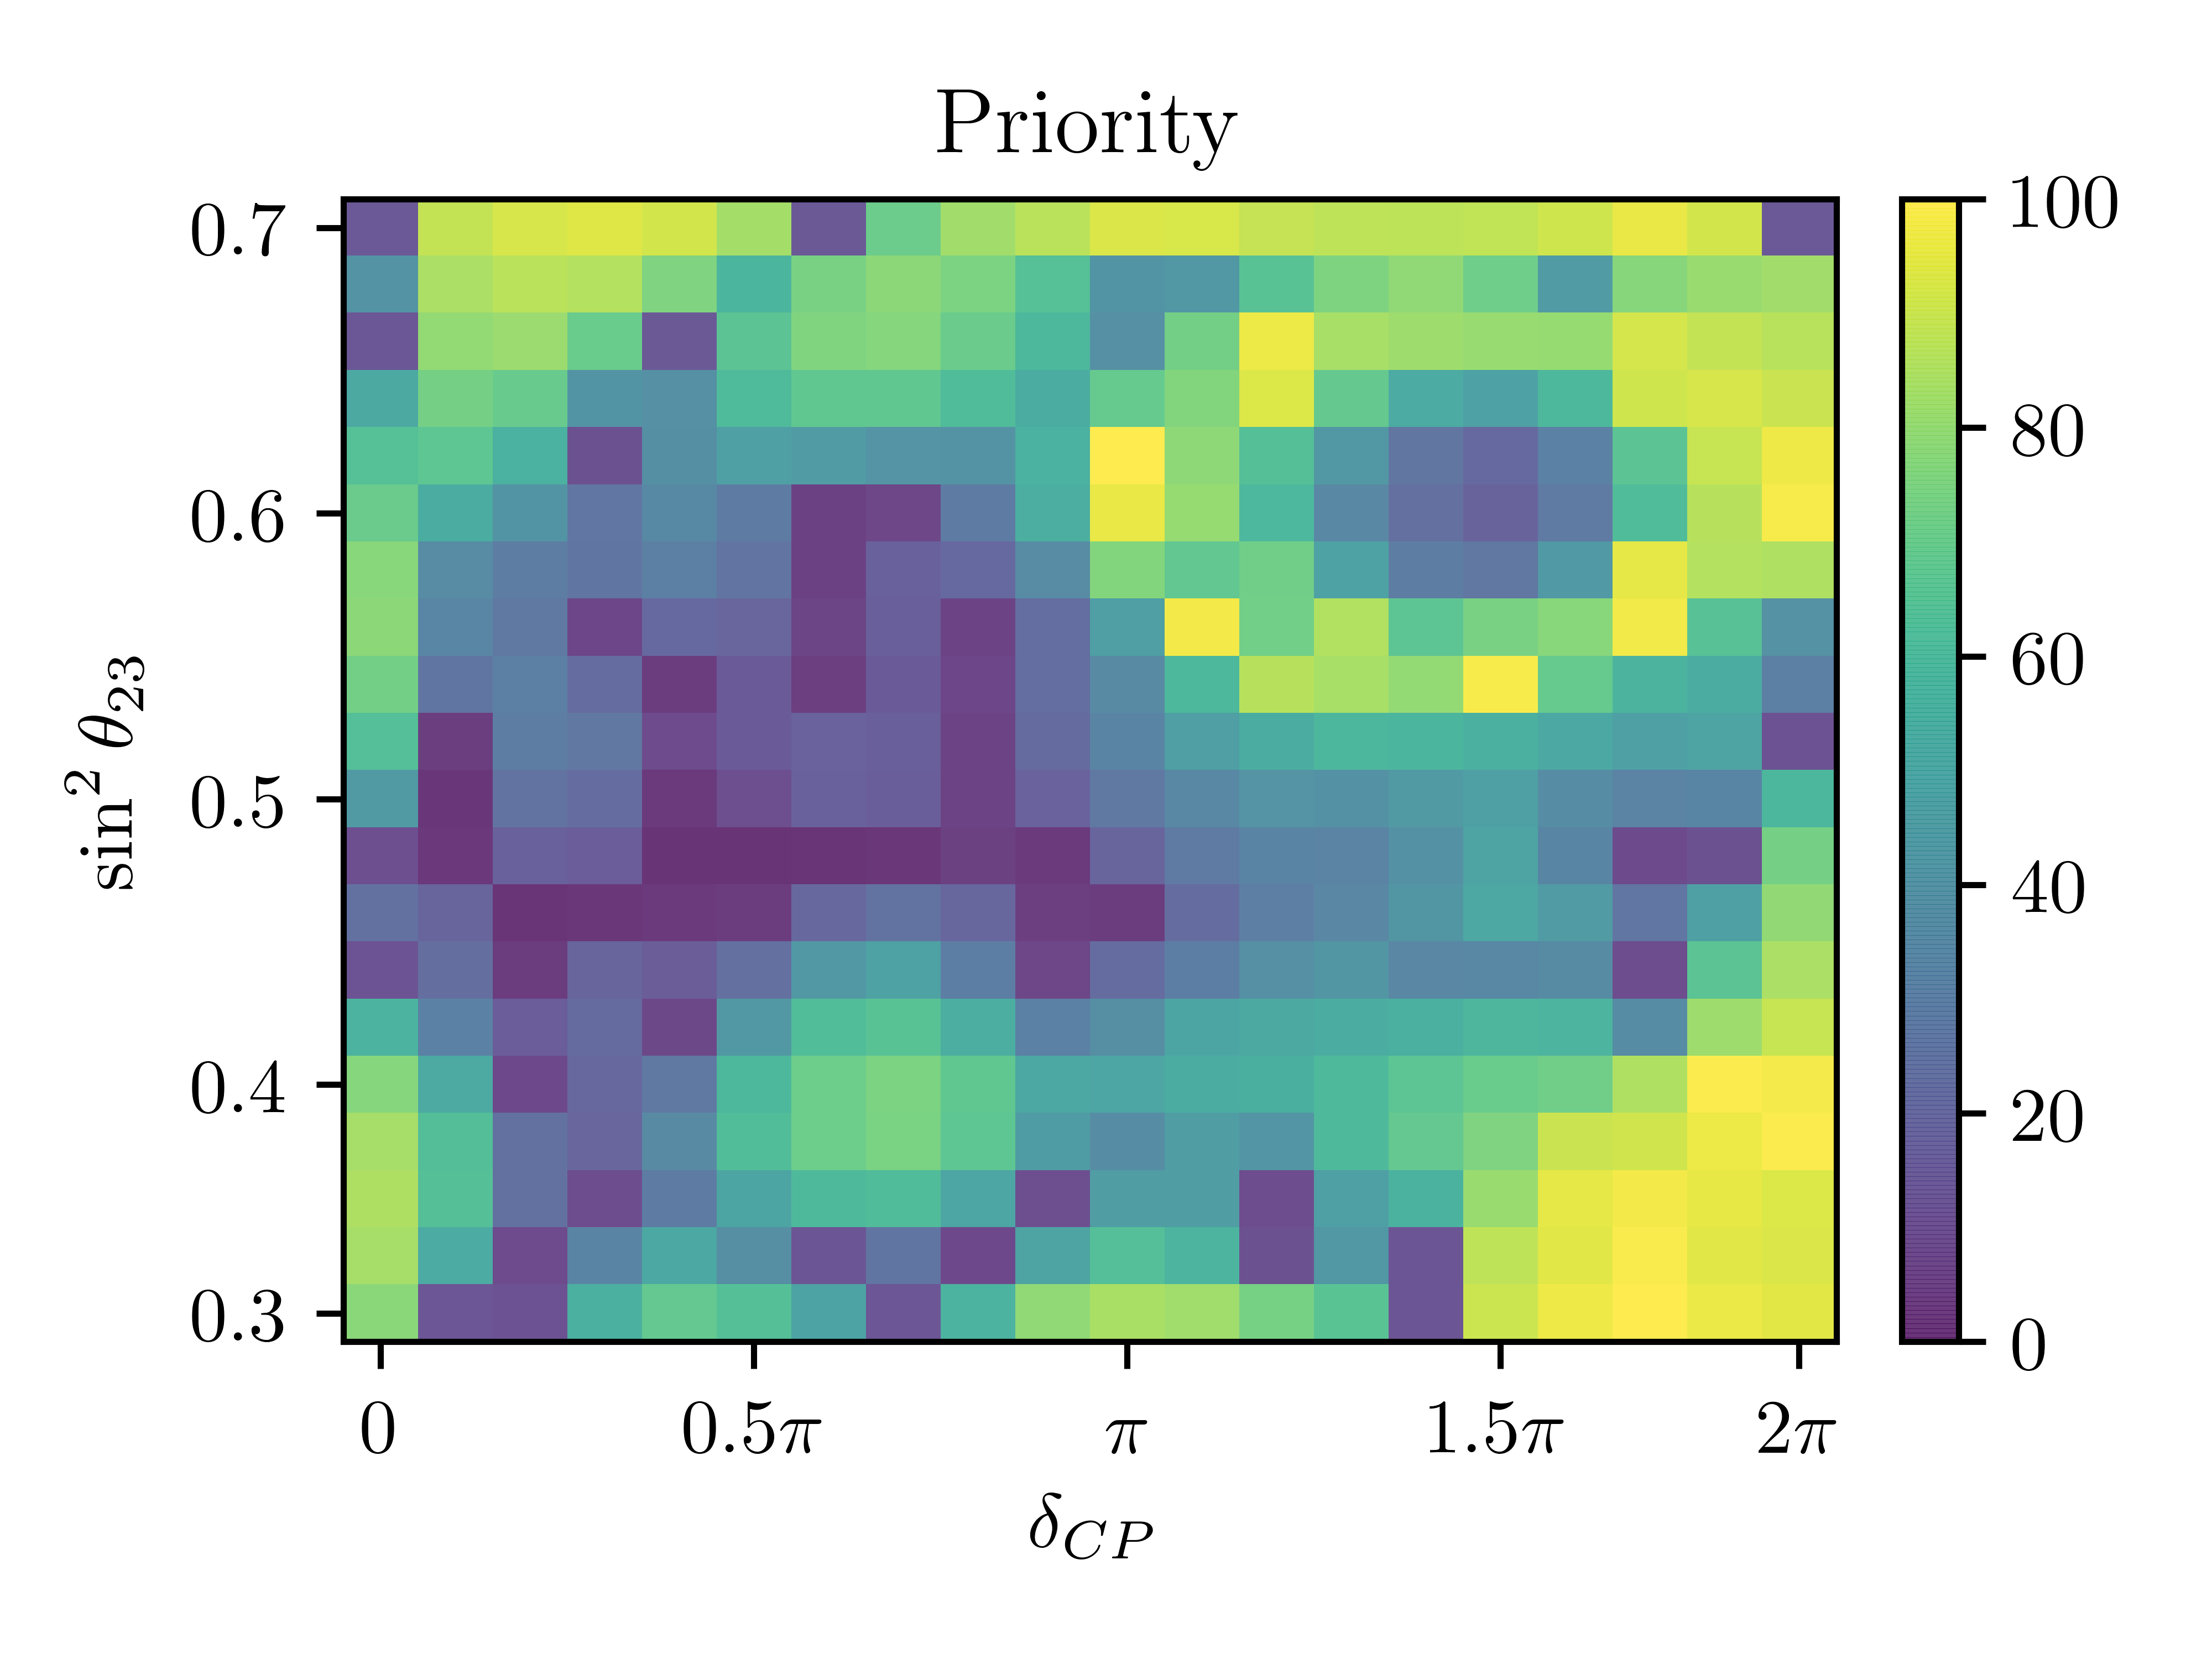
\includegraphics[scale=0.6]{figures_final/priority_2d_sdcp_inverted_start.png}
    % 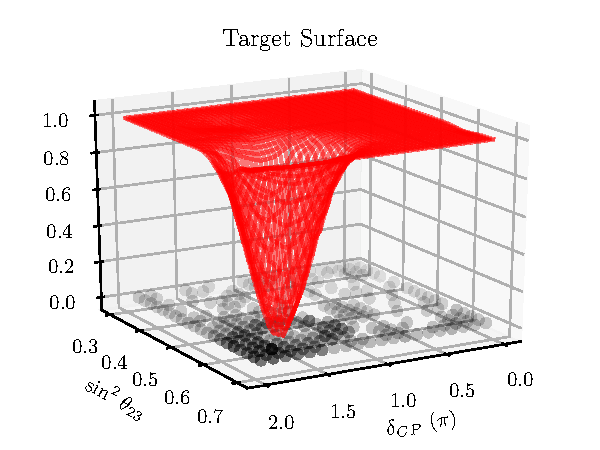
\includegraphics[scale=0.6]{figures_final/target_sdcp_inverted.pdf}
    % \column{0.5\textwidth}
    % 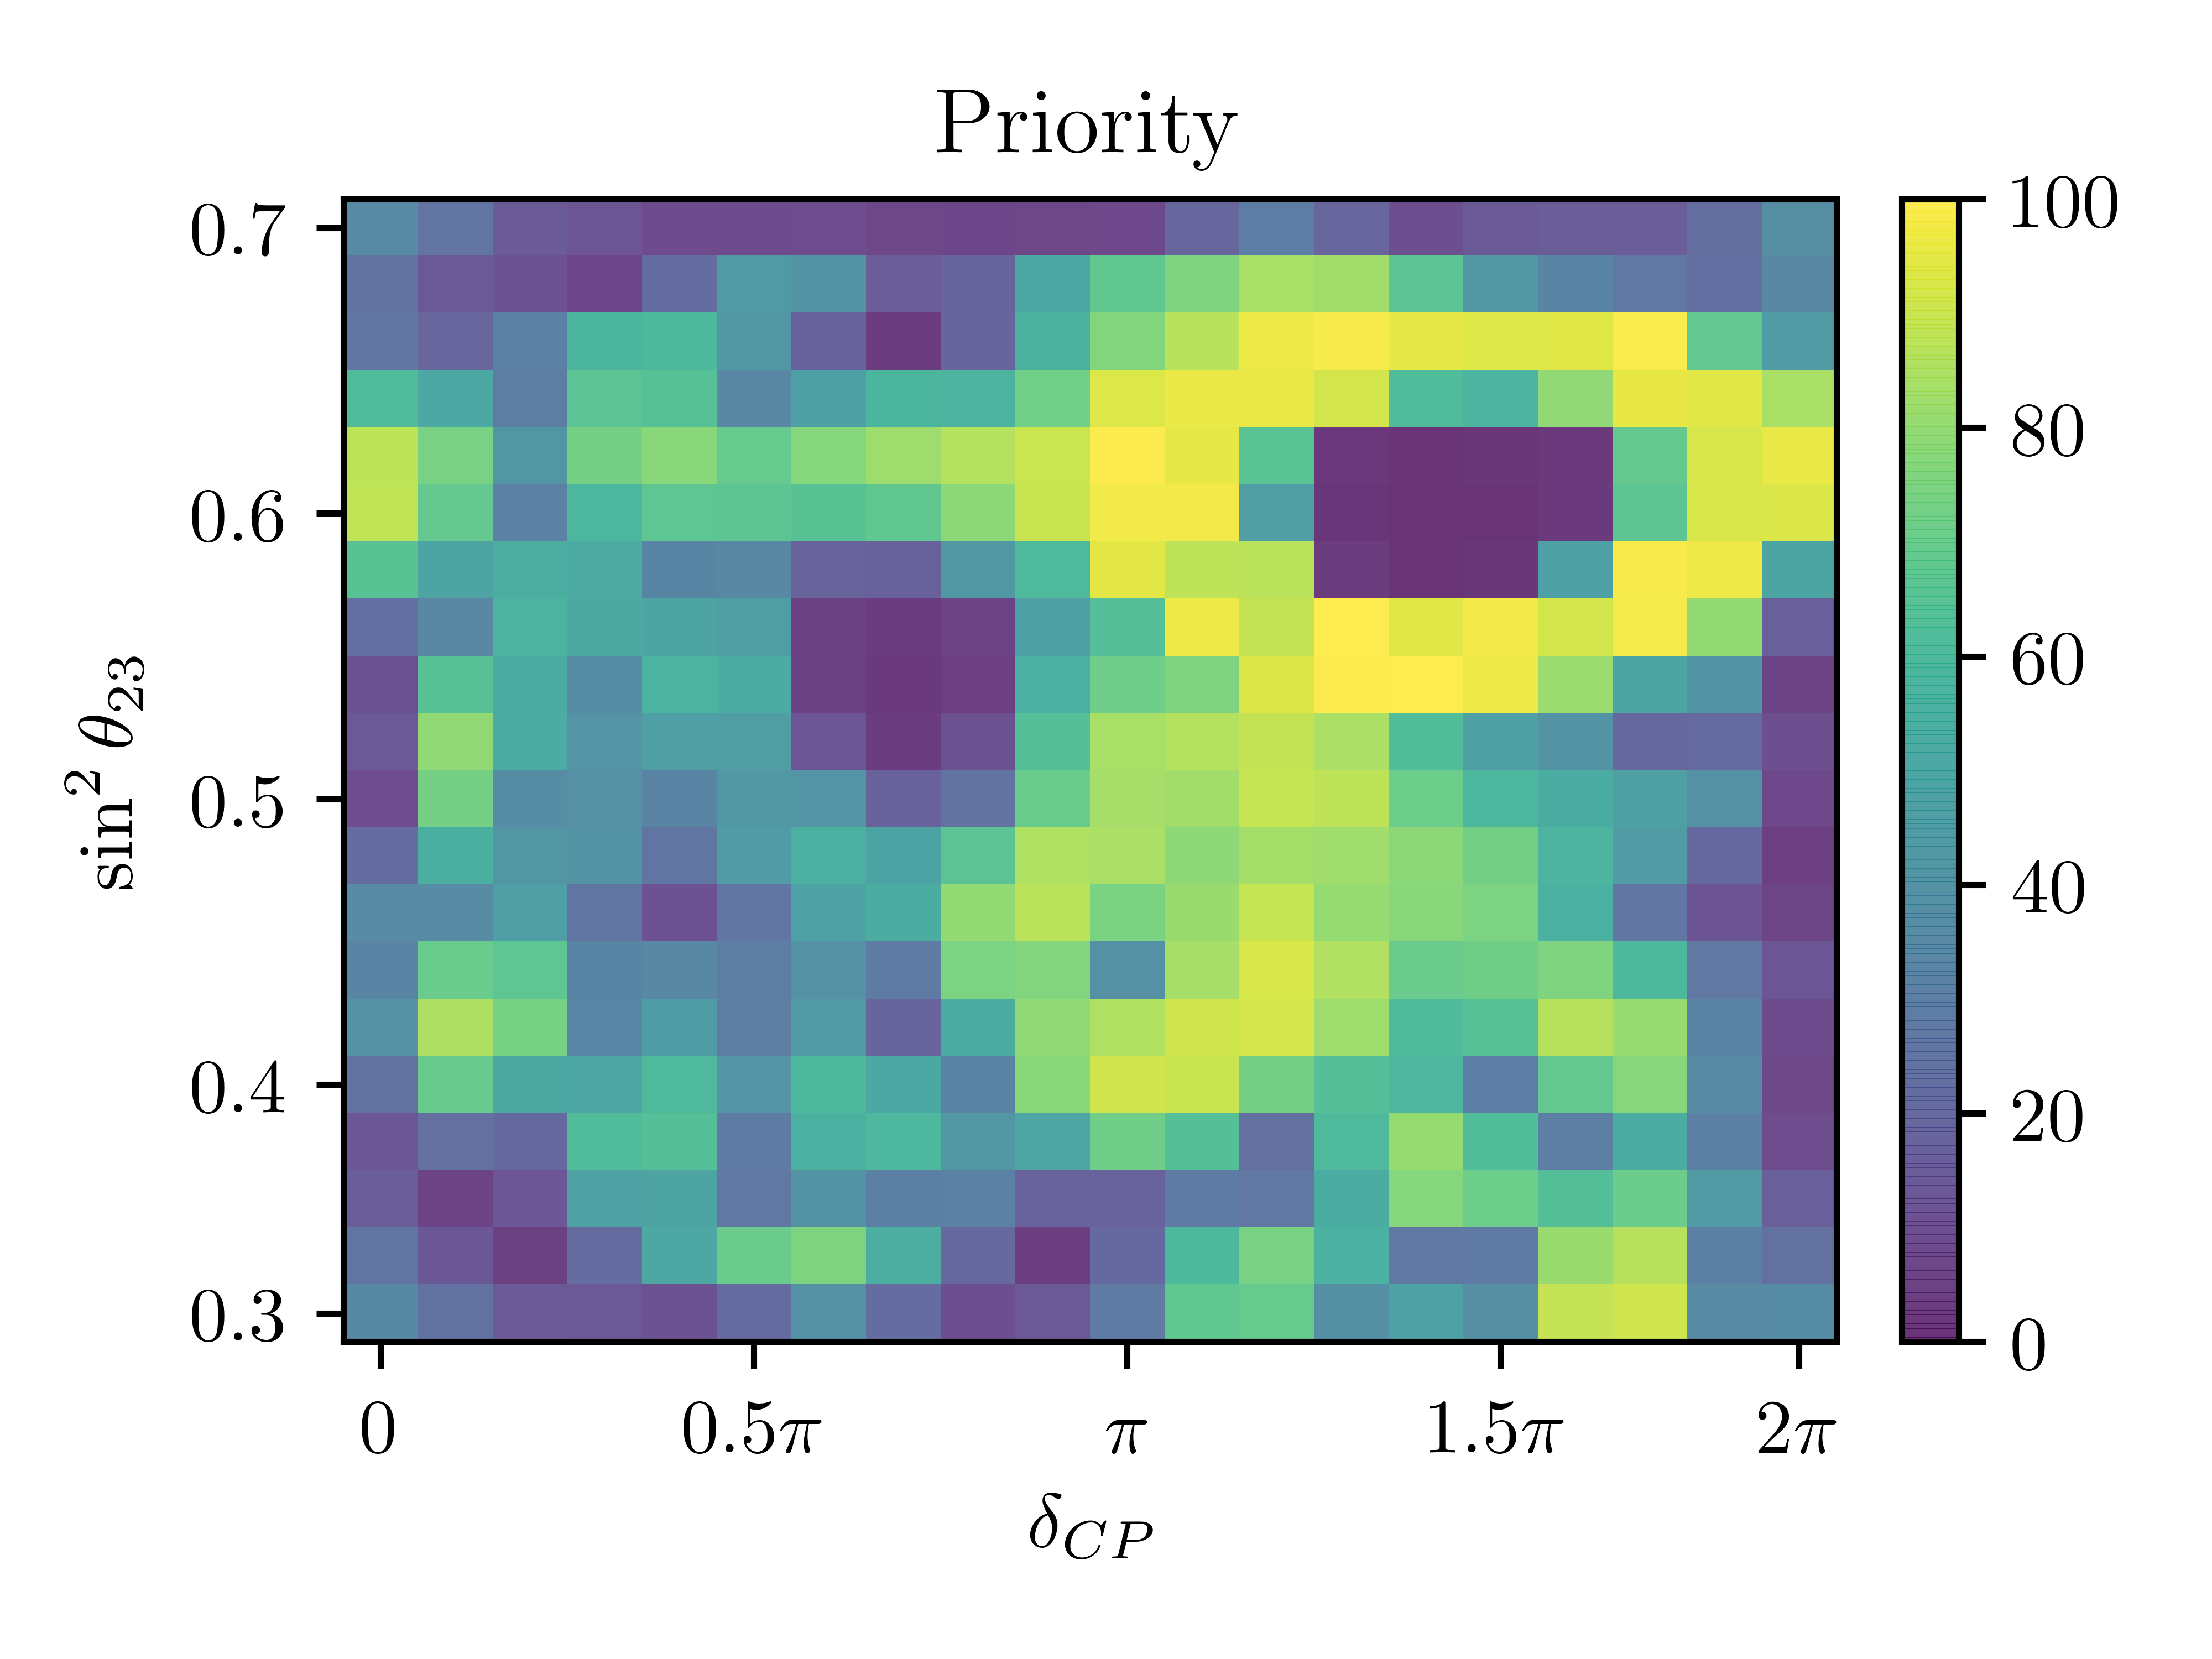
\includegraphics[scale=0.6]{figures_final/priority_2d_sdcp_inverted.png}
  \end{columns}
\end{frame}
\begin{frame}
  \frametitle{Optimised Confidence Interval Search}
  \begin{itemize}
    \item Use an acquisition function that proposes new points in $\theta$-space to explore based on $\mathcal{GP}$ approximated percentile surface.
      \begin{equation*}
    a(\theta) = \sum_{\alpha_i}|\frac{\hat{q}(\theta)-\alpha_i}{\sigma_{\hat{q}(\theta)}}|^{-1}
      \end{equation*}
    \item Here, $\hat{q}(\theta)$ is $\mathcal{GP}$ mean, $\sigma_{\hat{q}(\theta)}$ is $\mathcal{GP}$ std-dev, $\alpha_i$ is chosen to be $(0.68, 0.90)$
    \item $a(\theta)$ balances between exploration, i.e MC experiments at new points and exploitation, i.e reducing $\mathcal{GP}$ error
  \end{itemize}
  \begin{columns}
    \column{0.5\textwidth}
    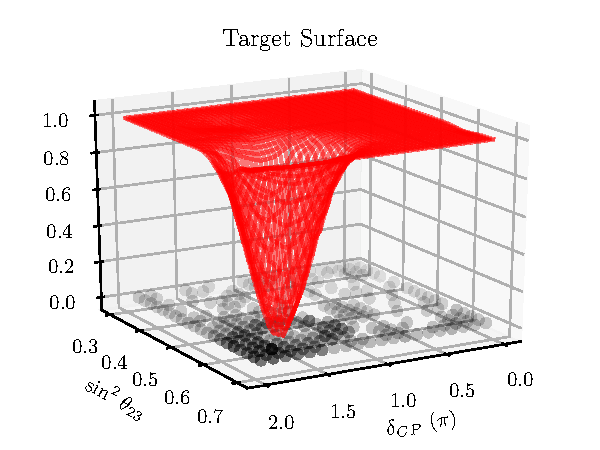
\includegraphics[scale=0.6]{figures_final/target_sdcp_inverted.pdf}
    \column{0.5\textwidth}
    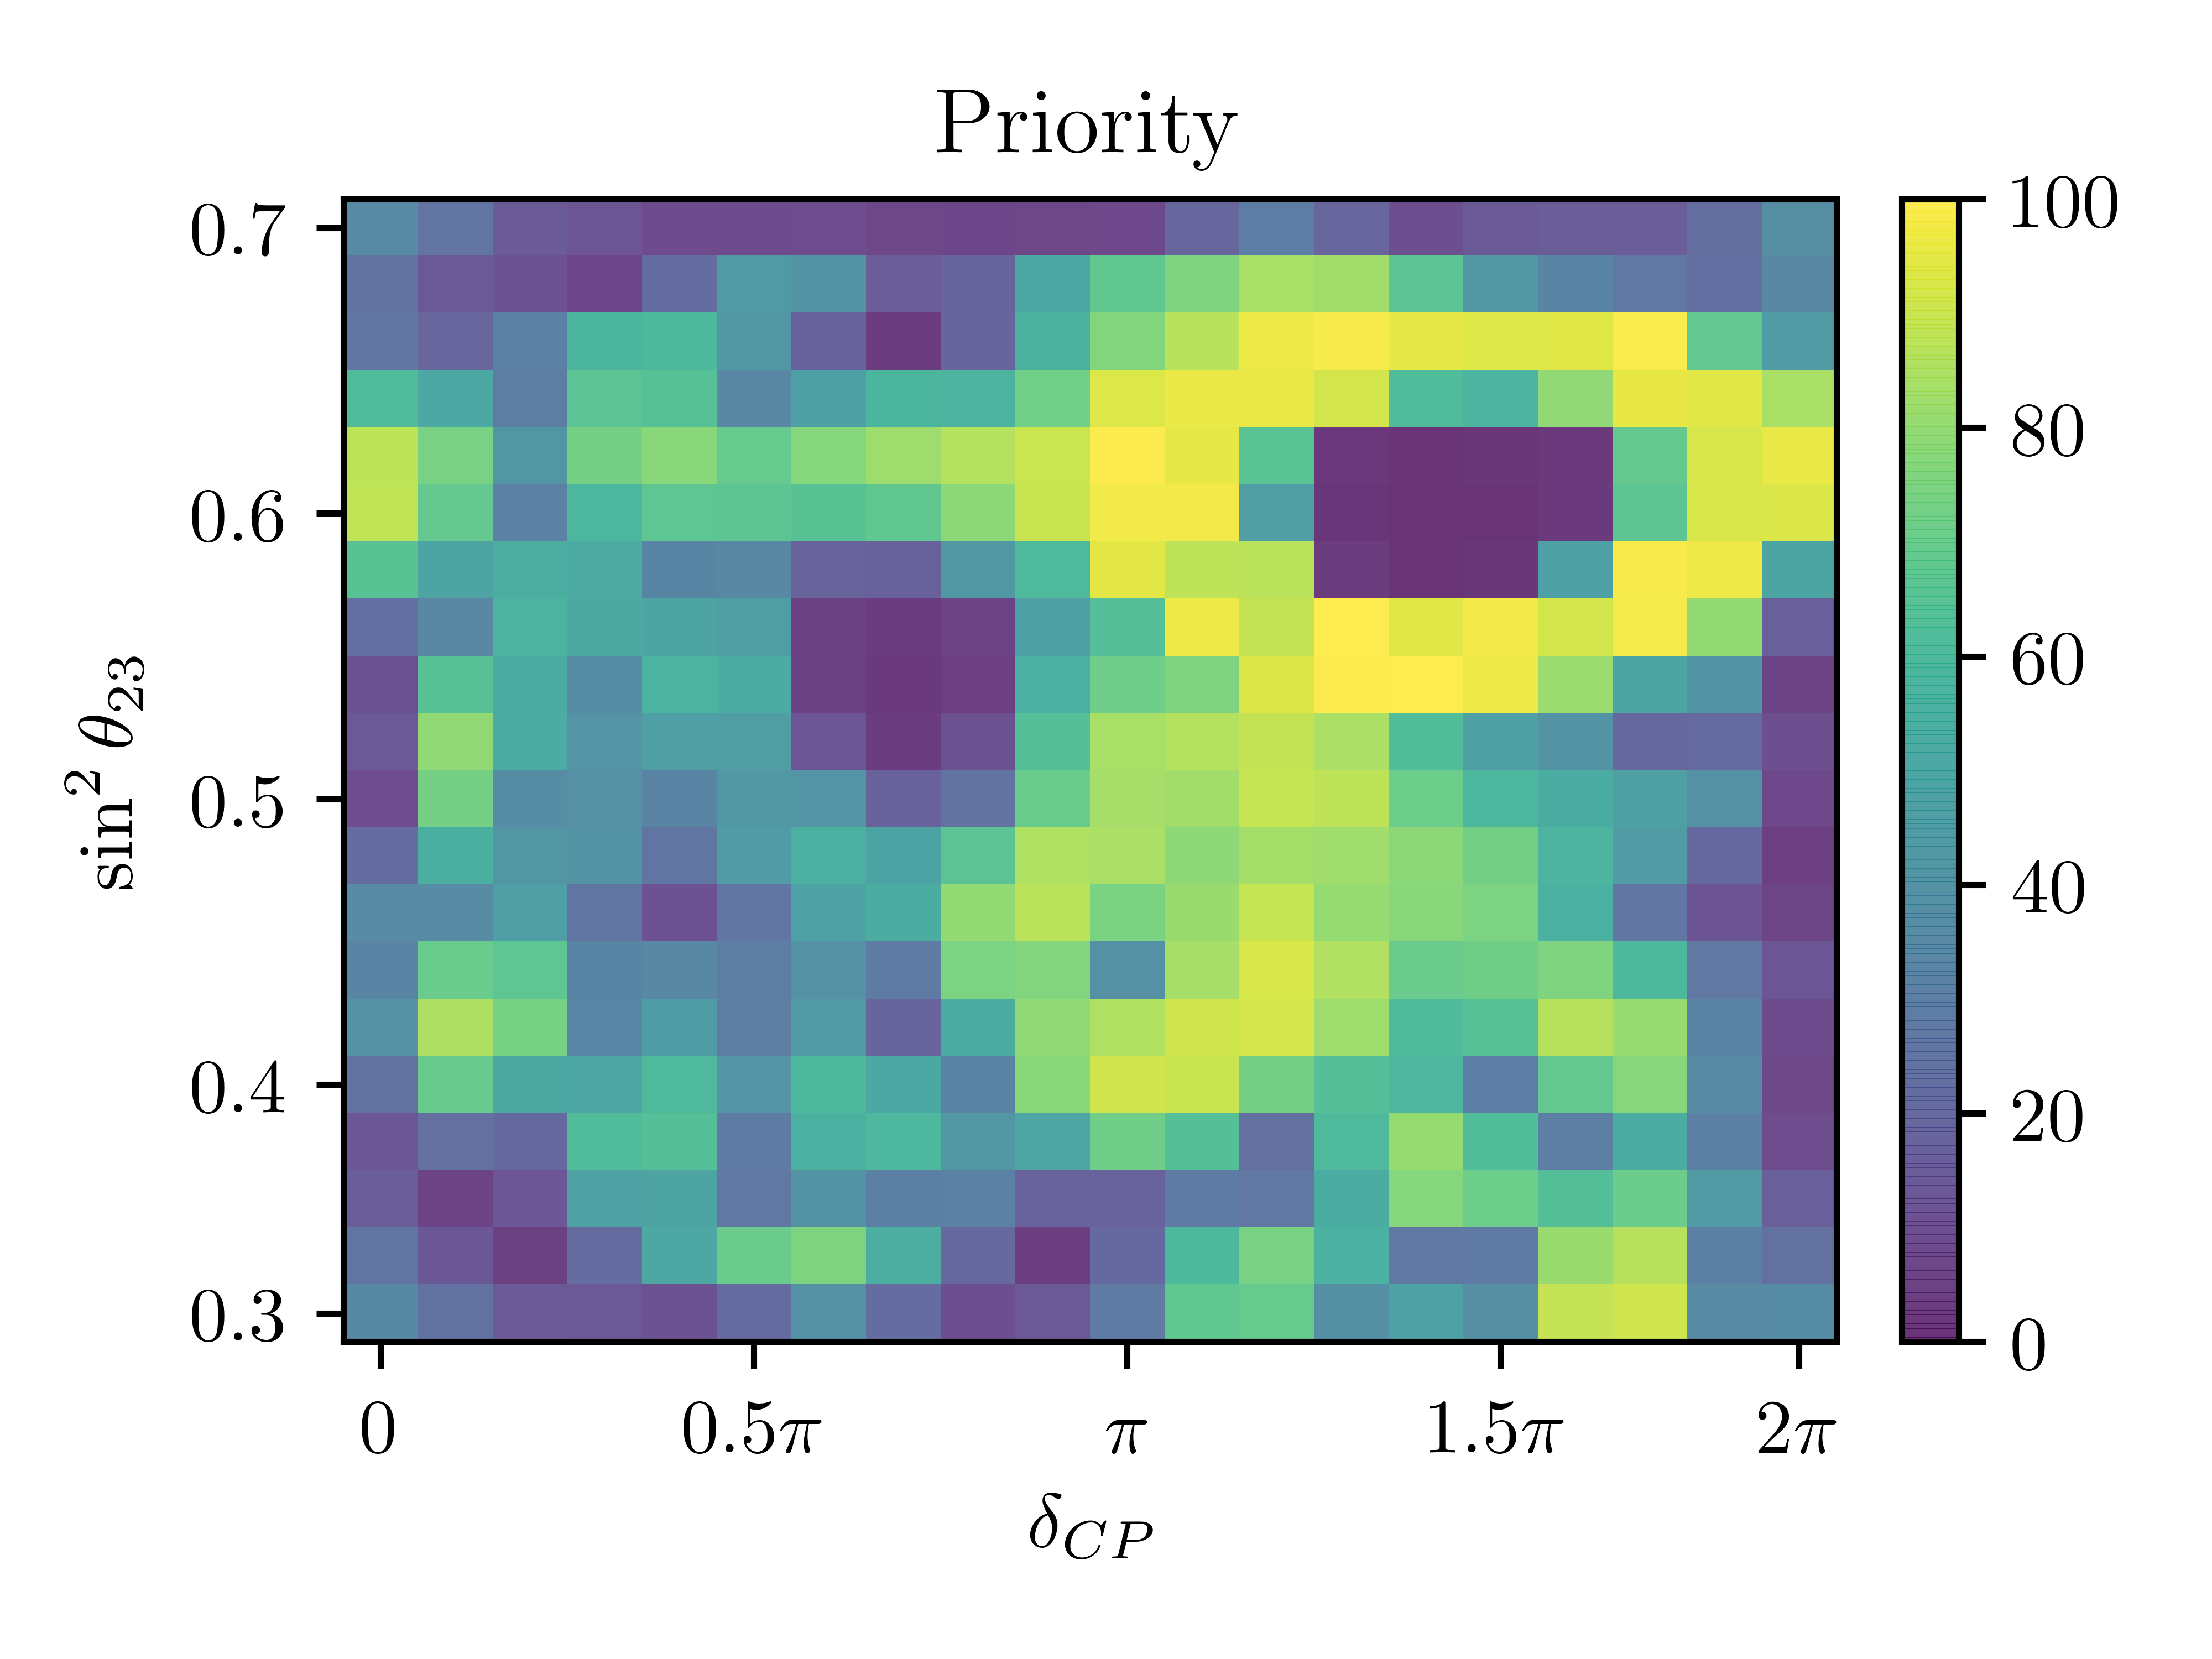
\includegraphics[scale=0.6]{figures_final/priority_2d_sdcp_inverted.png}
  \end{columns}
\end{frame}
\begin{frame}
  \frametitle{Results}
  \begin{itemize}
    \item "Real" data similar to latest best-fit estimate from NOvA. ($sin^{2}\theta_{23} = 0.56$, $\Delta m^2_{32} = 2.44\times10^{-3} eV^{2}$, $\delta_{CP} = 1.5\pi$)
    \item $sin^{2}\theta_{23}-\delta_{CP}$ 68\% and 90\% CI for IH after 5 iterations
  \end{itemize}
  \begin{columns}
    \column{0.5\textwidth}
    % 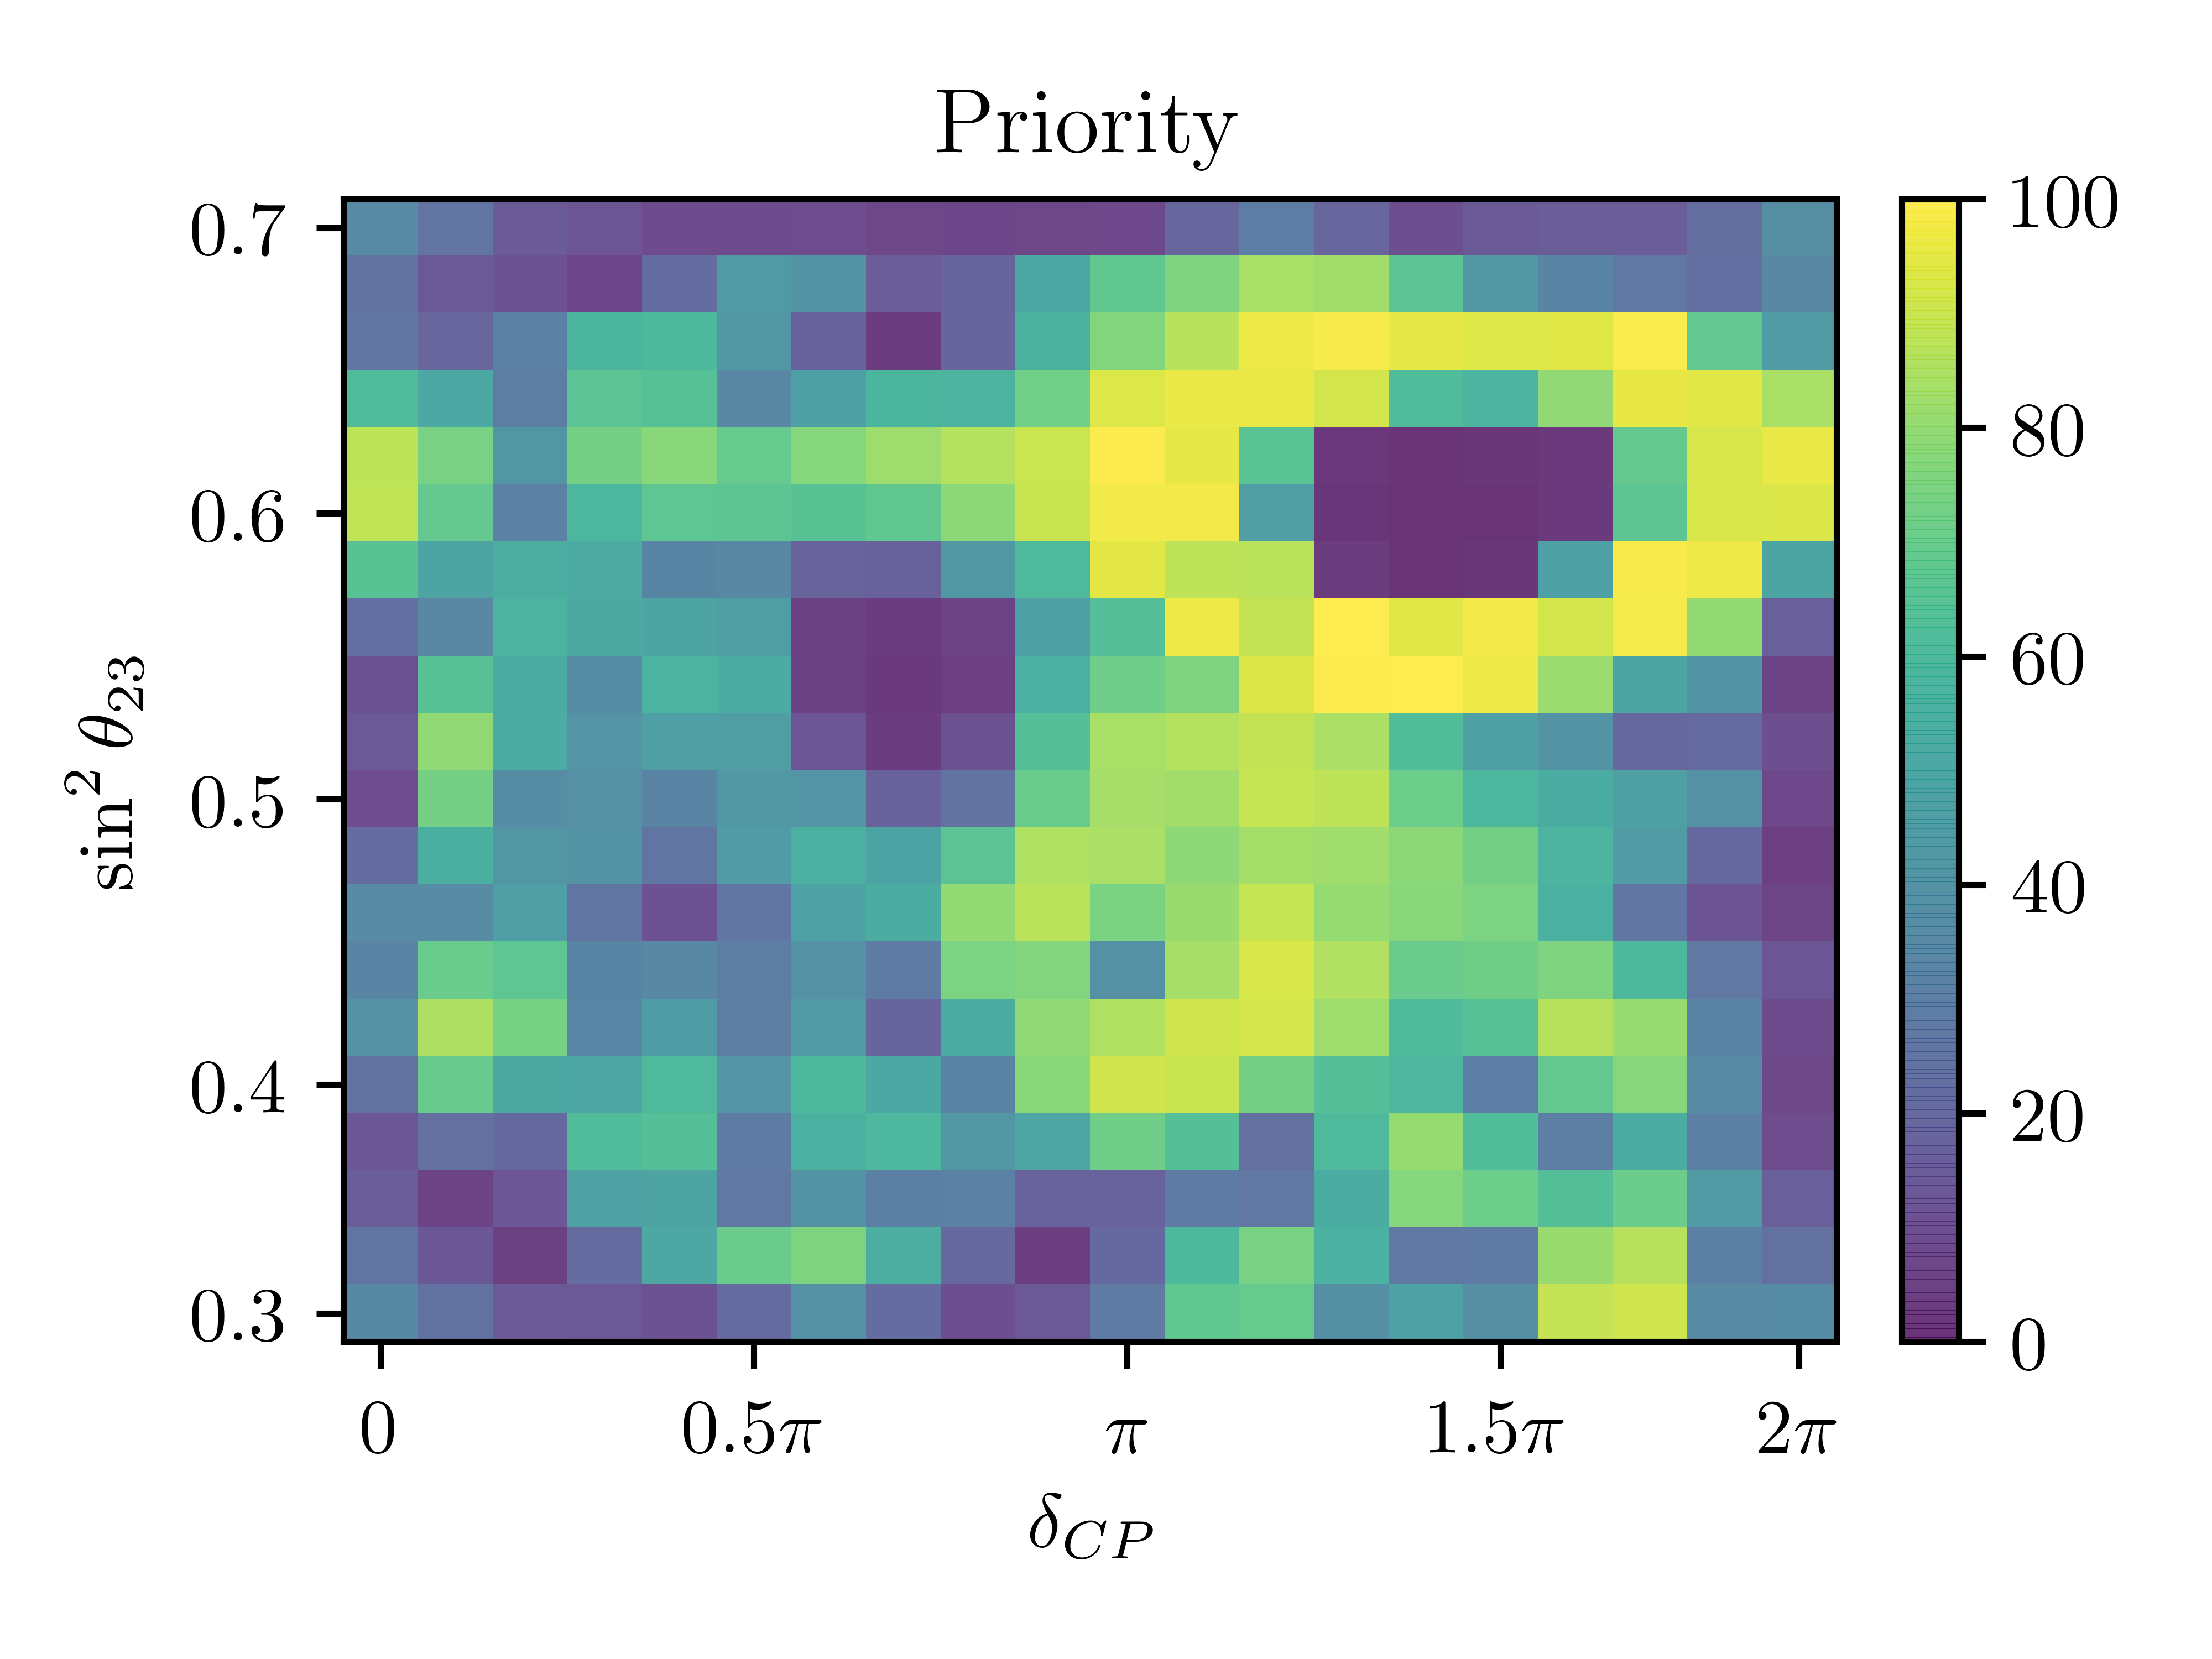
\includegraphics[scale=0.45]{figures_final/priority_2d_sdcp_inverted.png}
    \centering{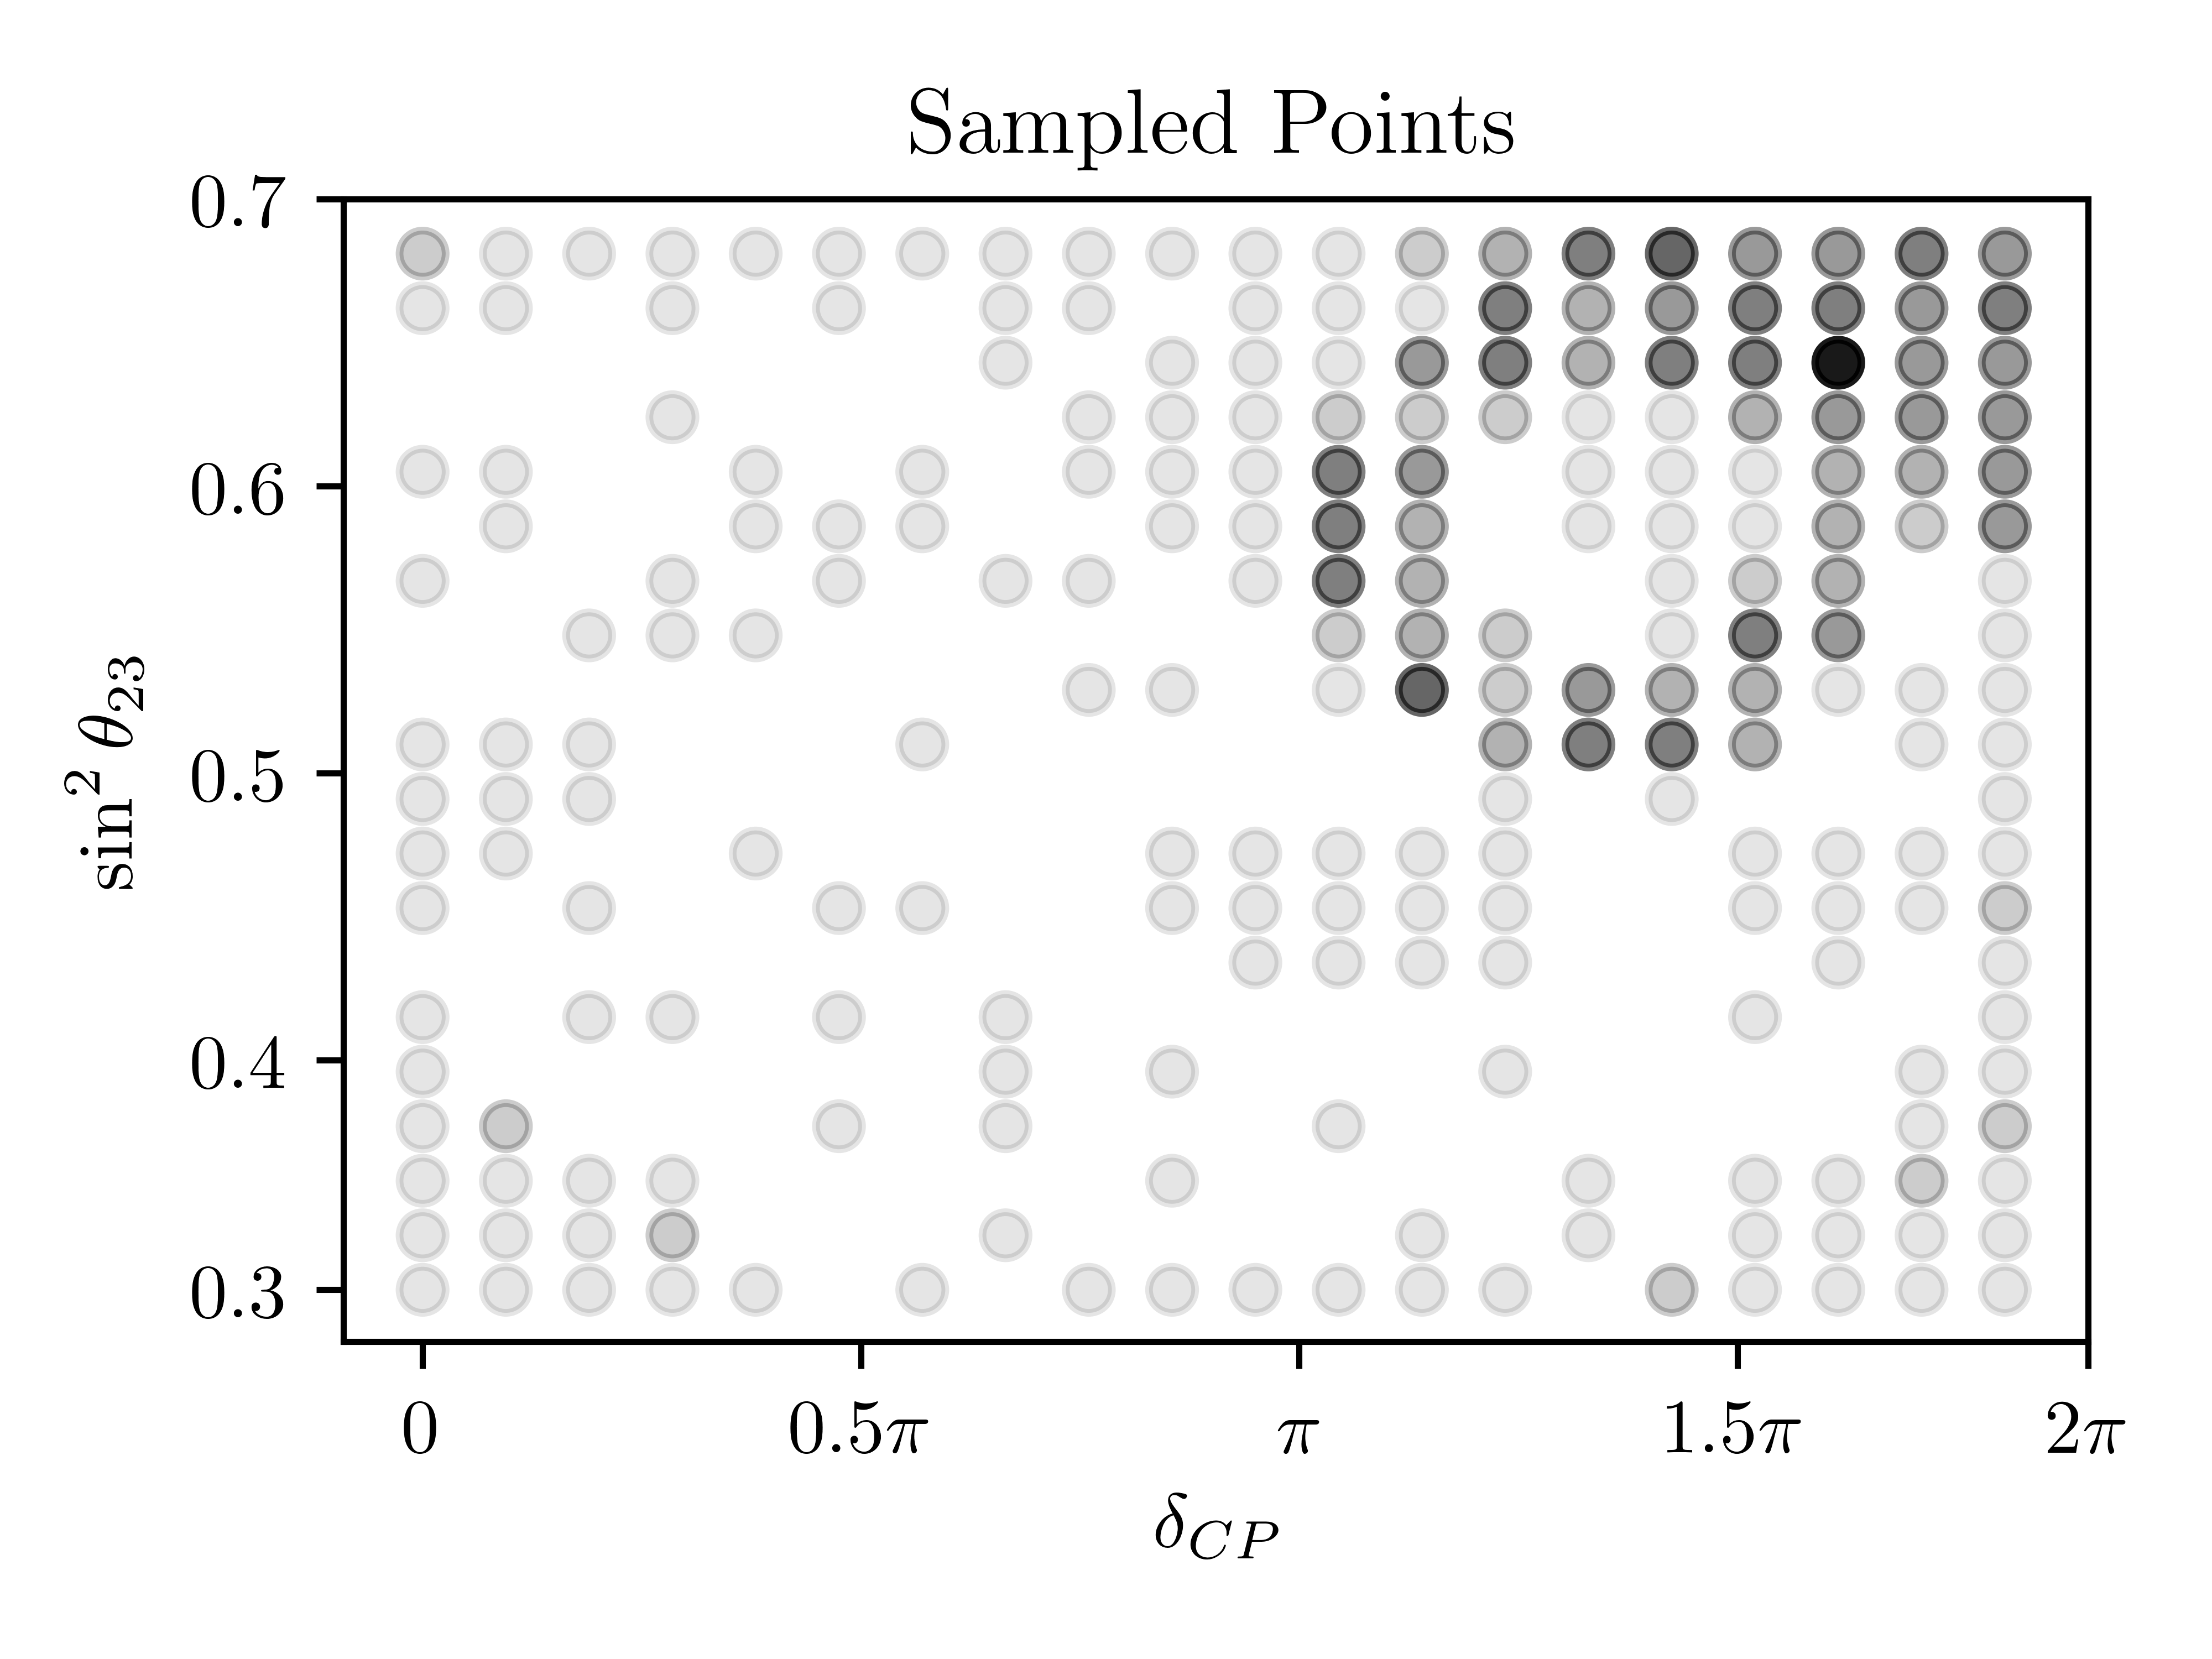
\includegraphics[scale=0.6]{figures_final/sample_2d_sdcp_inverted.png}}
    \column{0.5\textwidth}
    \centering{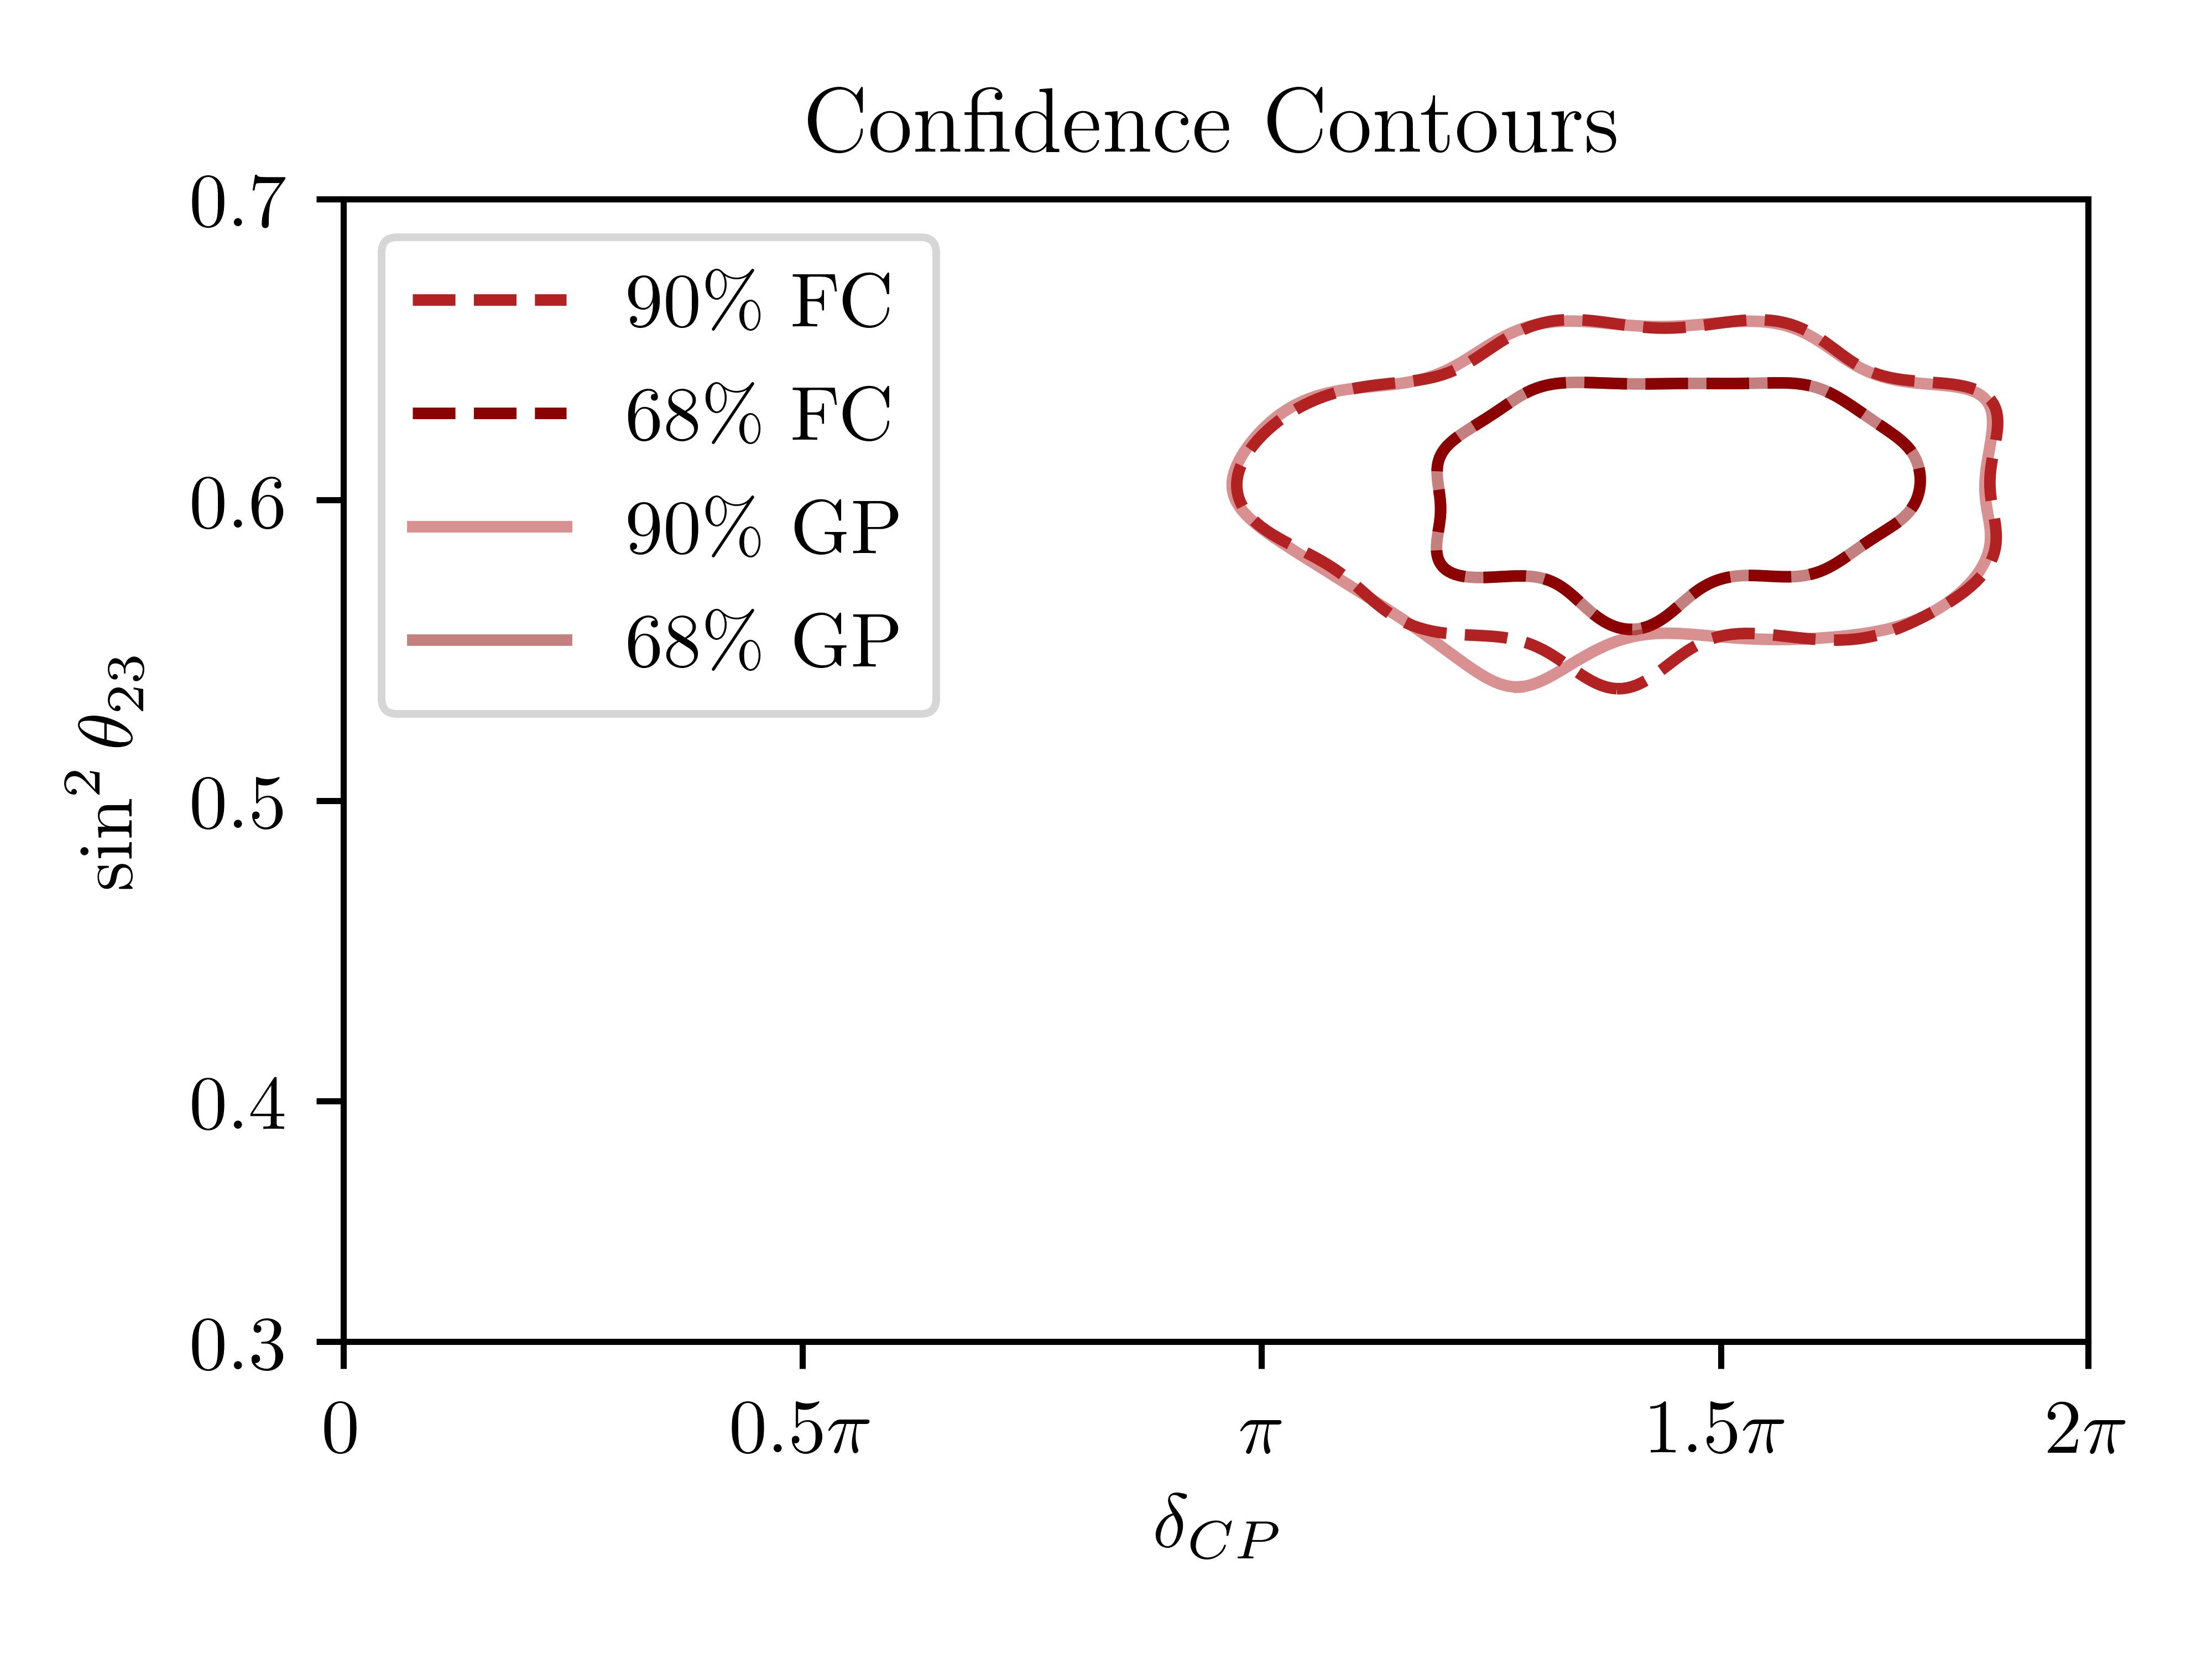
\includegraphics[scale=0.6]{figures_final/contour_2d_sdcp_inverted.png}}
  \end{columns}
  % \begin{columns}
  %   \column{0.5\textwidth}
  %   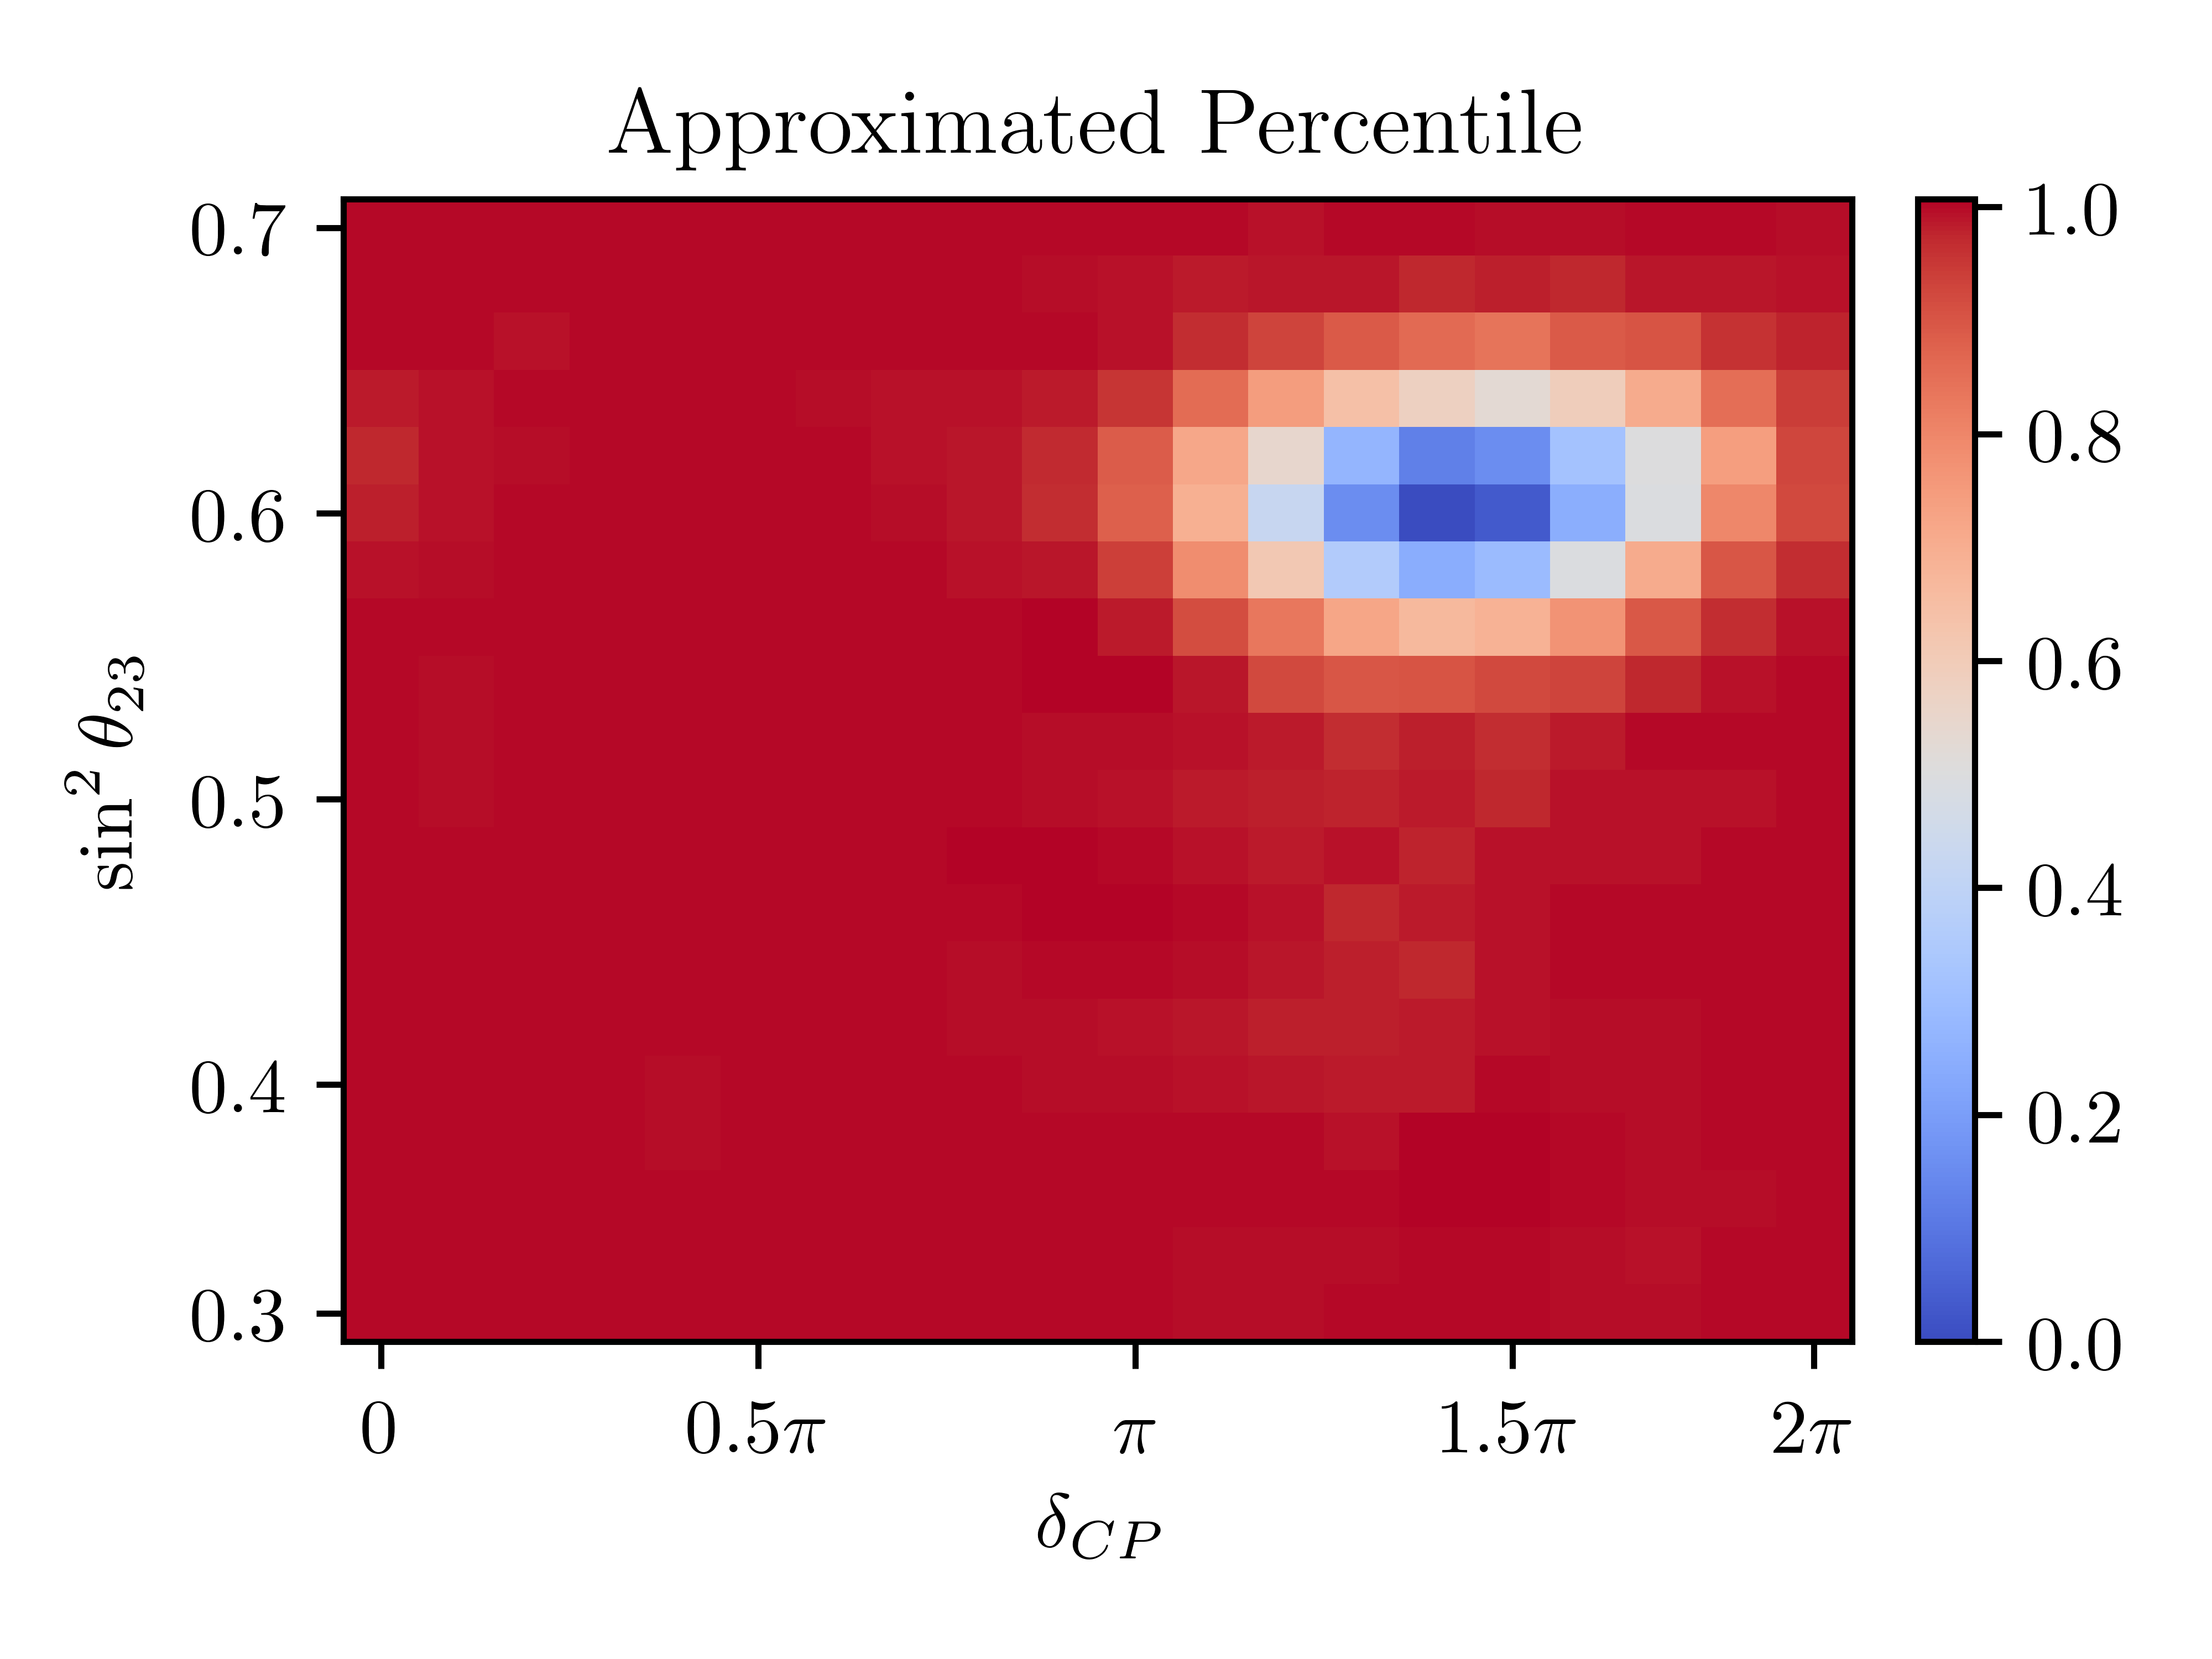
\includegraphics[scale=0.45]{figures_final/approximation_2d_sdcp_inverted.png}
  %   \column{0.5\textwidth}
  % \end{columns}
  \begin{itemize}
    \item Grayscale denotes number of experiments thrown in relation to FC ($2000$)
    \item Algorithm does a good job of finding the FC contour edge!  
  \end{itemize}
\end{frame}

\begin{frame}
  \frametitle{Results}
  \begin{itemize}
    \item "Real" data similar to latest best-fit estimate from NOvA. ($sin^{2}\theta_{23} = 0.56$, $\Delta m^2_{32} = 2.44\times10^{-3} eV^{2}$, $\delta_{CP} = 1.5\pi$)
    \item $sin^{2}\theta_{23}-\delta_{CP}$ 68\% and 90\% CI for NH after 5 iterations
  \end{itemize}
  \begin{columns}
    \column{0.5\textwidth}
    \centering{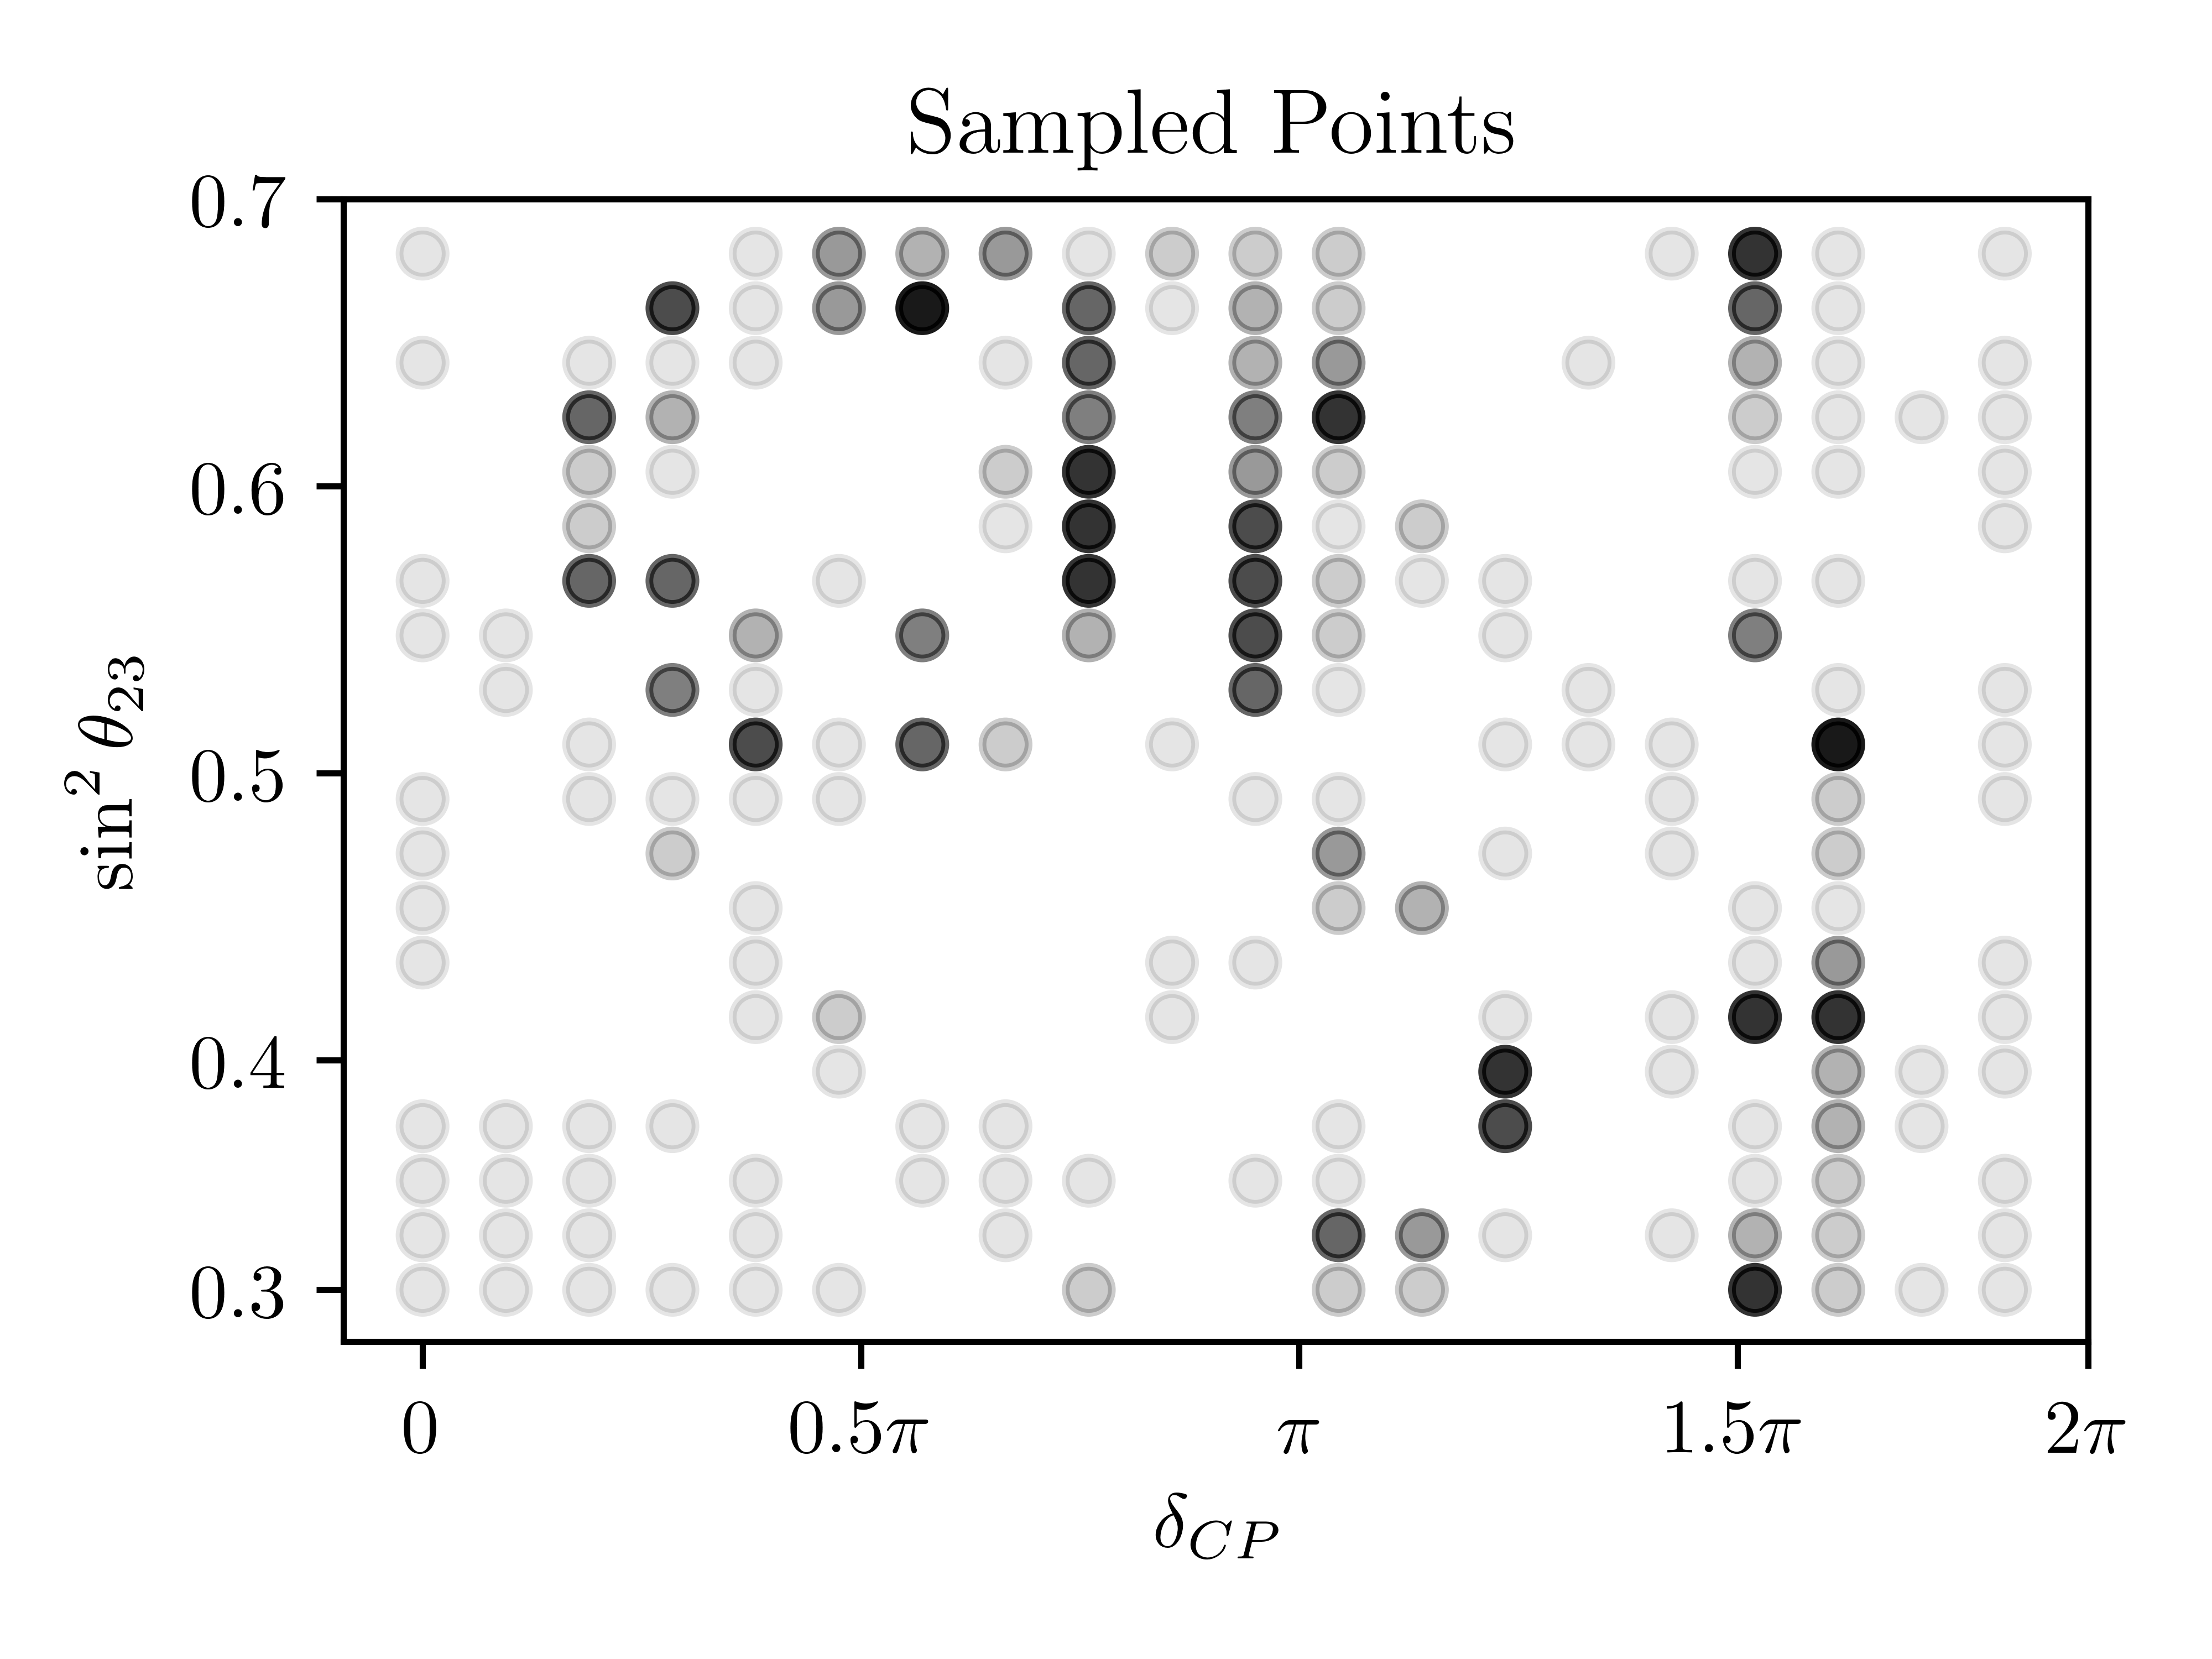
\includegraphics[scale=0.6]{figures_final/sample_2d_sdcp.png}}
    \column{0.5\textwidth}
    \centering{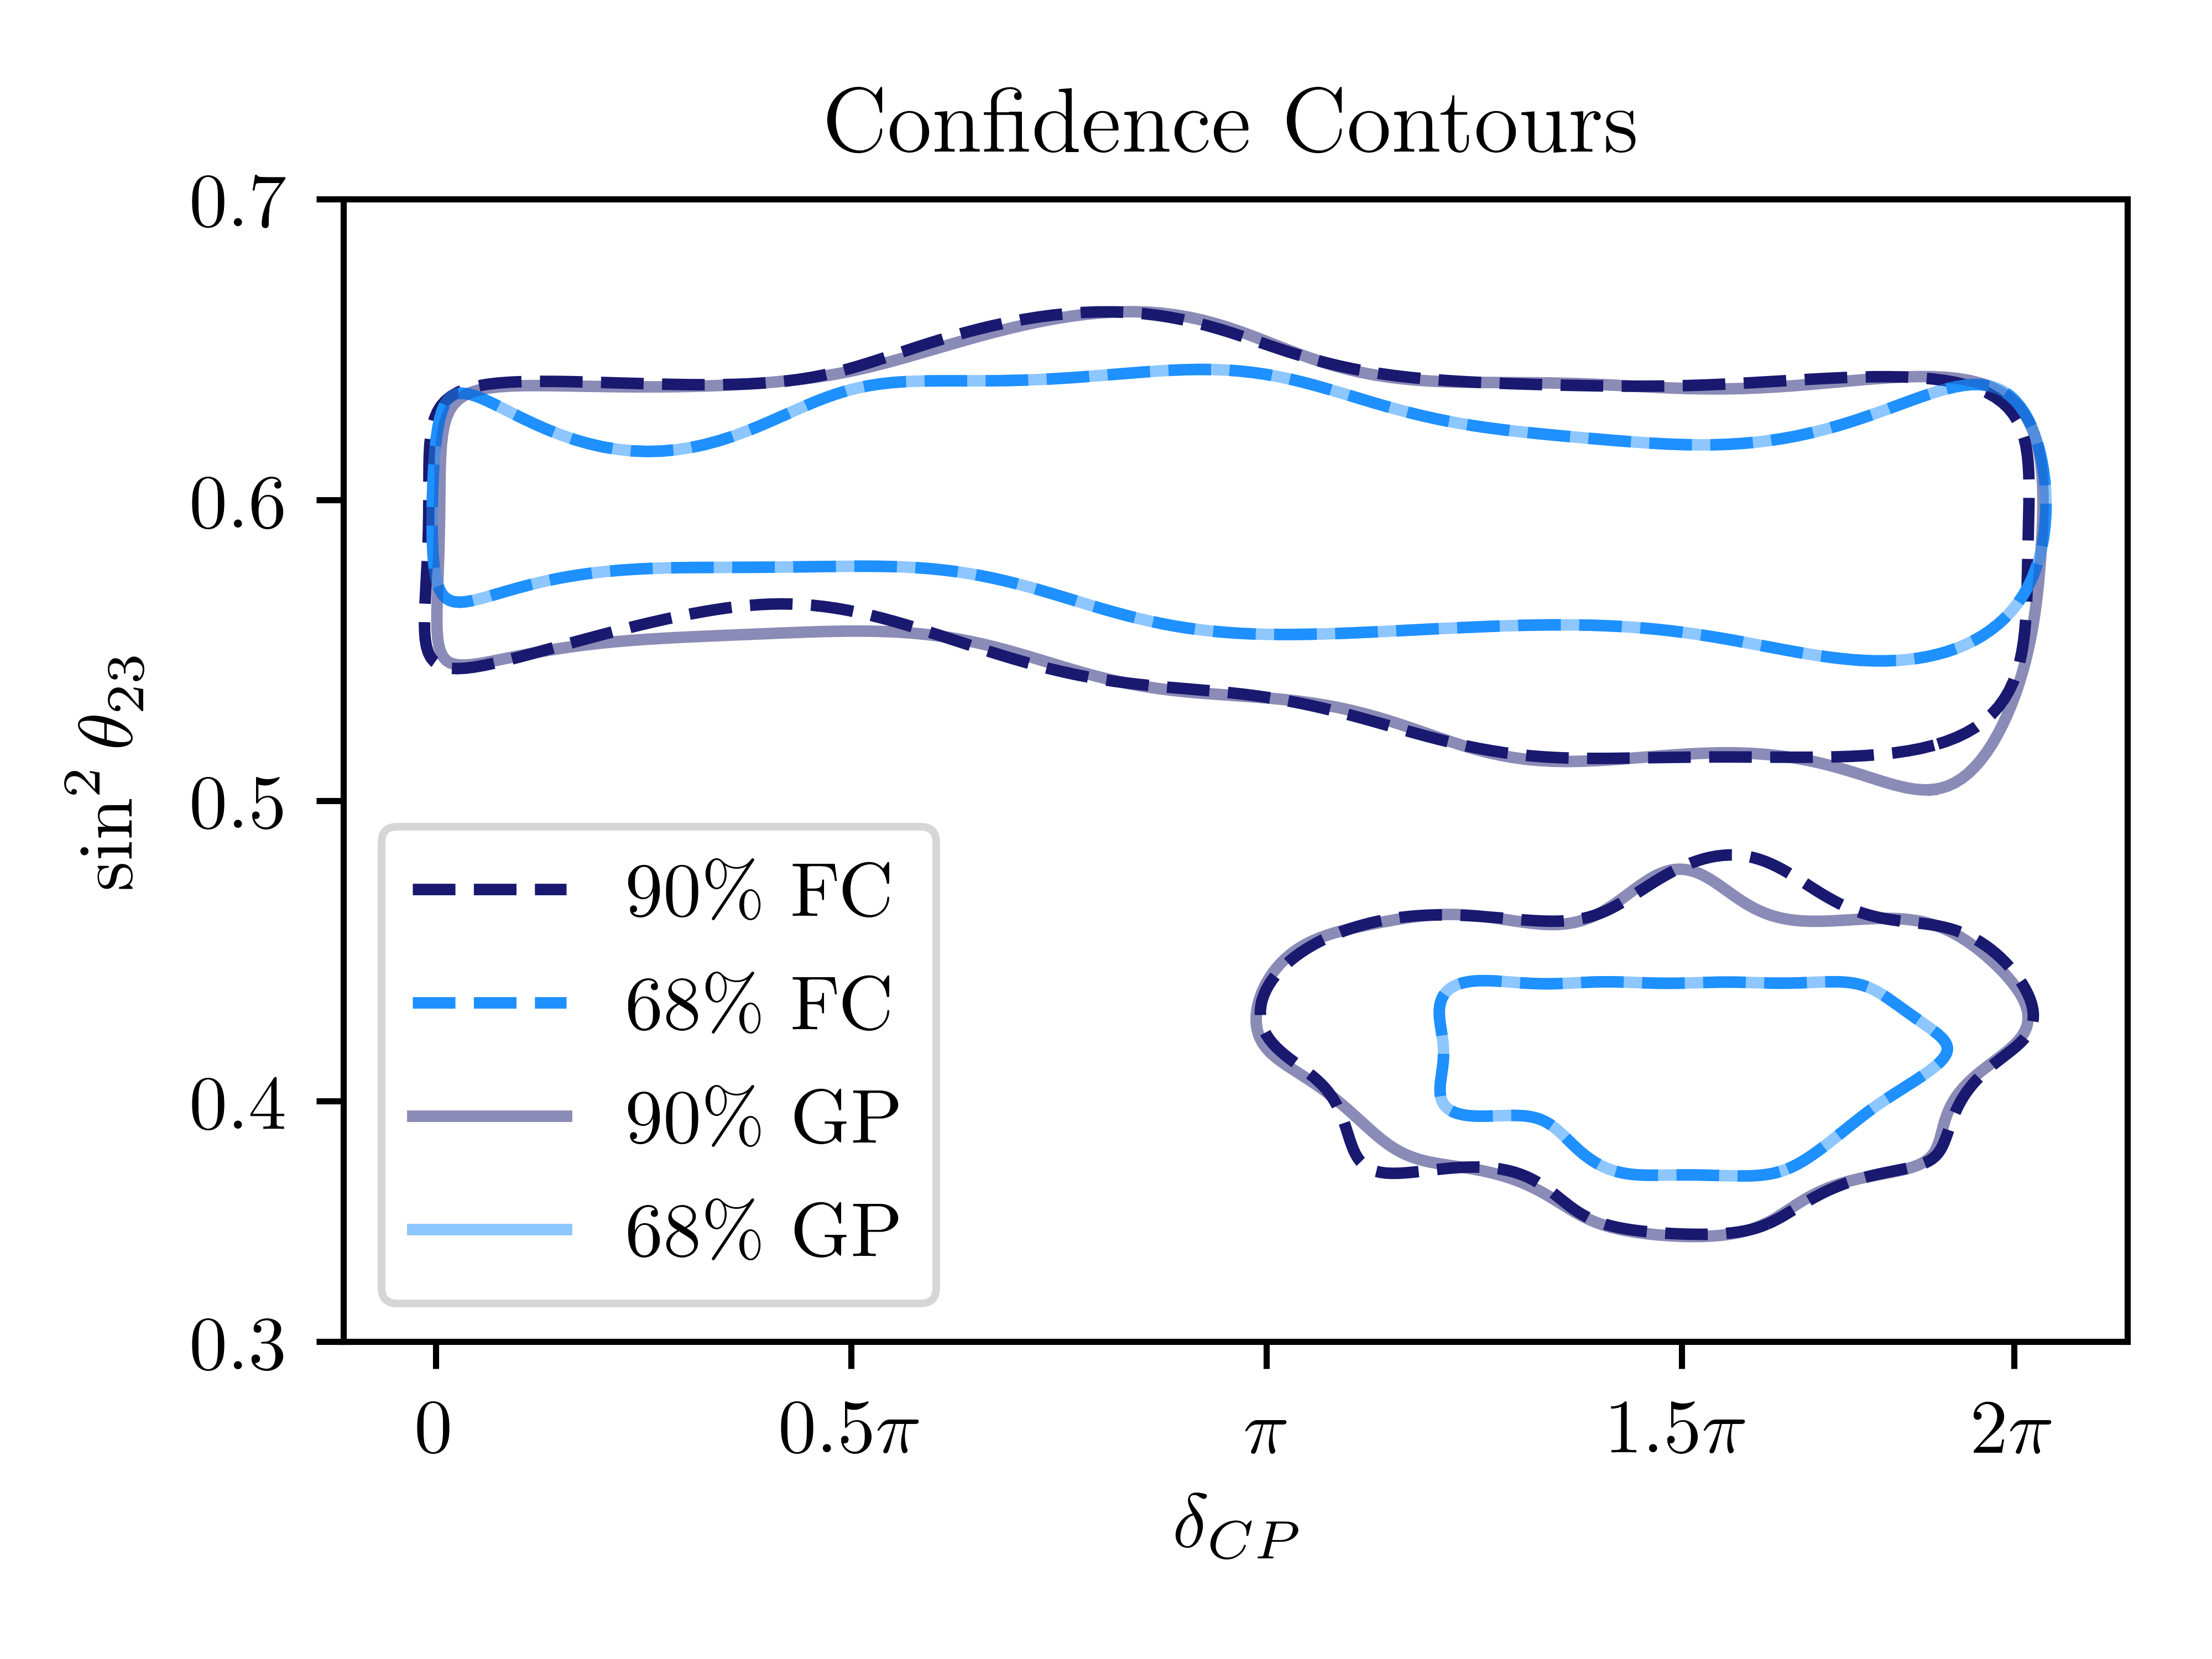
\includegraphics[scale=0.6]{figures_final/contour_2d_sdcp.png}}
  \end{columns}
\end{frame}

\begin{frame}
  \frametitle{Results}
  \begin{itemize}
    \item "Real" data similar to latest best-fit estimate from NOvA. ($sin^{2}\theta_{23} = 0.56$, $\Delta m^2_{32} = 2.44\times10^{-3} eV^{2}$, $\delta_{CP} = 1.5\pi$)
    \item Significance of rejecting $\delta_{CP}$ only after 5 iterations. (Percentile converted to Z-score significance) 
  \end{itemize}
  \begin{columns}
    \column{0.5\textwidth}
    \centering{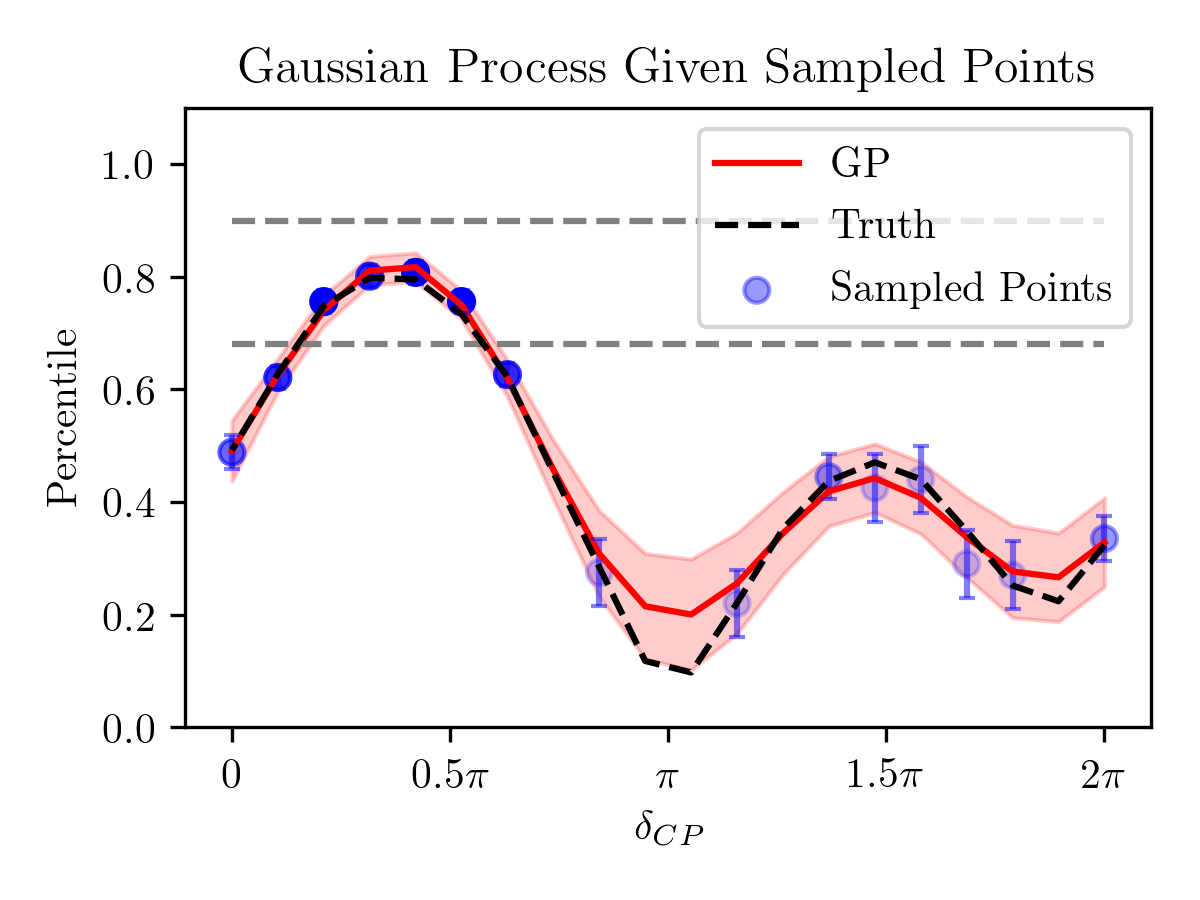
\includegraphics[scale=0.6]{figures_final/example_1d_end.png}}
    \column{0.5\textwidth}
    \centering{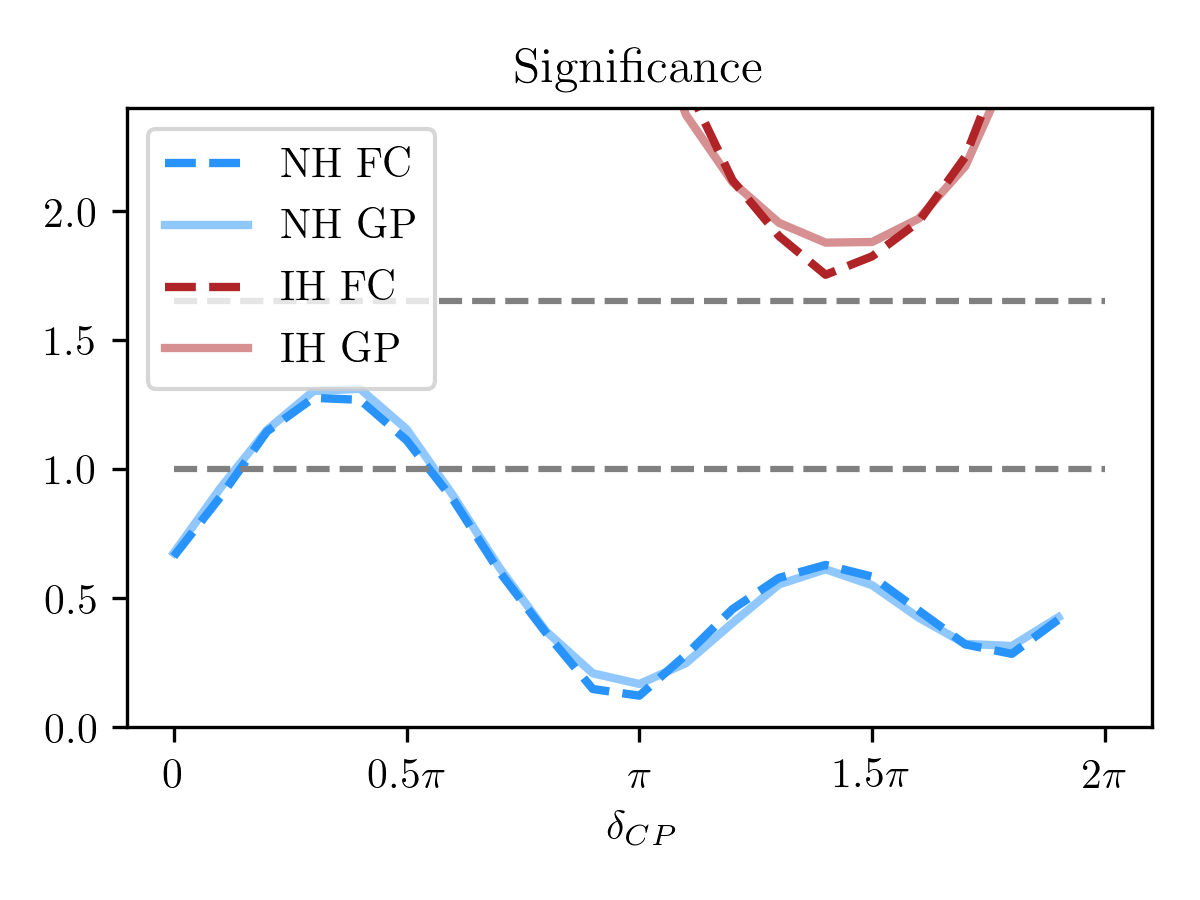
\includegraphics[scale=0.15]{figures_final/sig_1d.png}}
  \end{columns}
\end{frame}

\begin{frame}
  \frametitle{Results}
  \begin{itemize}
    \item 200 different runs for "real" data at the same point as before.
    \item Use classification accuracy of all grid points, taking FC result as truth, to evaluate performance.
    \item Progress shows the search algorithm converges to the FC value $\sim10\times$ faster for 2D case and $\sim5\times$ for 1D case
  \end{itemize}
  \begin{columns}
    \column{0.5\textwidth}
    \centering{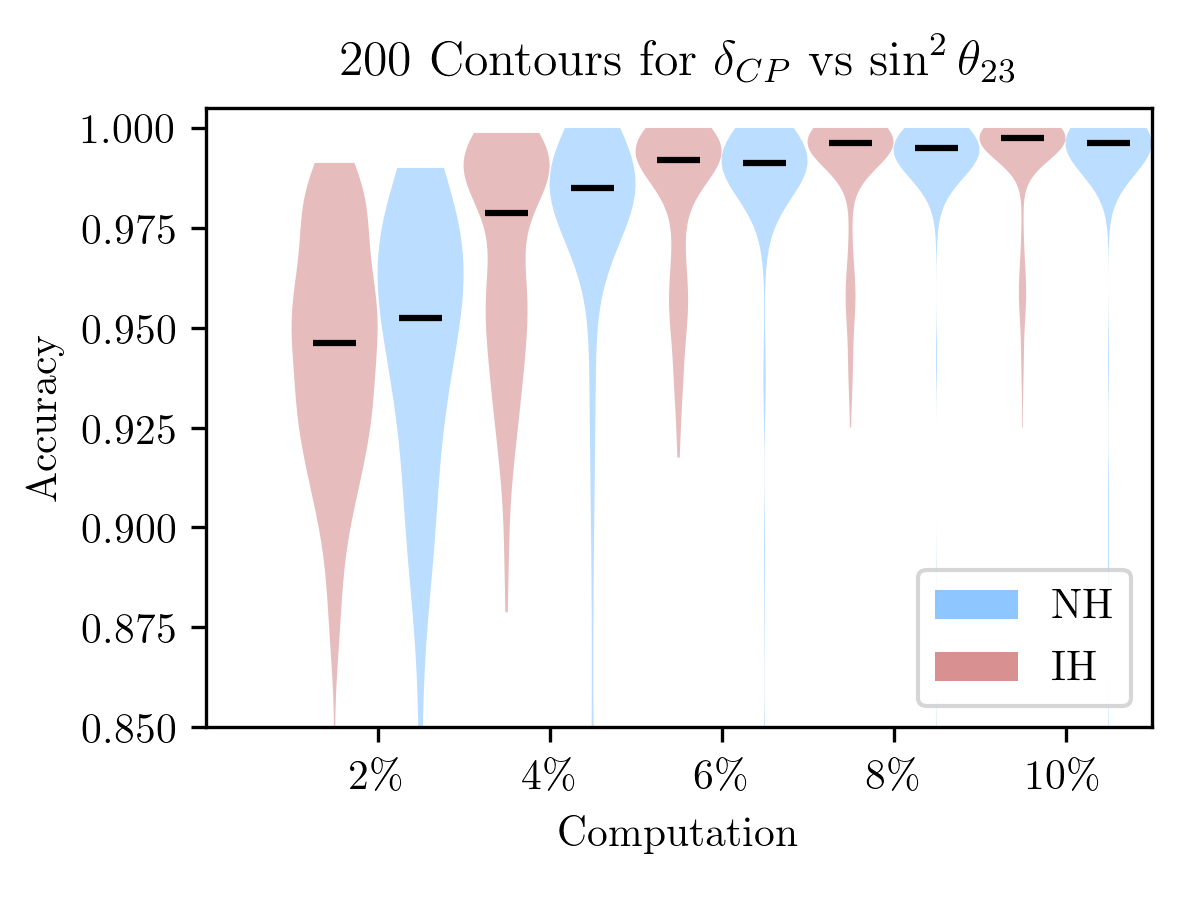
\includegraphics[scale=0.6]{figures_final/compare_contour_sdcp.png}}
    \column{0.5\textwidth}
    \centering{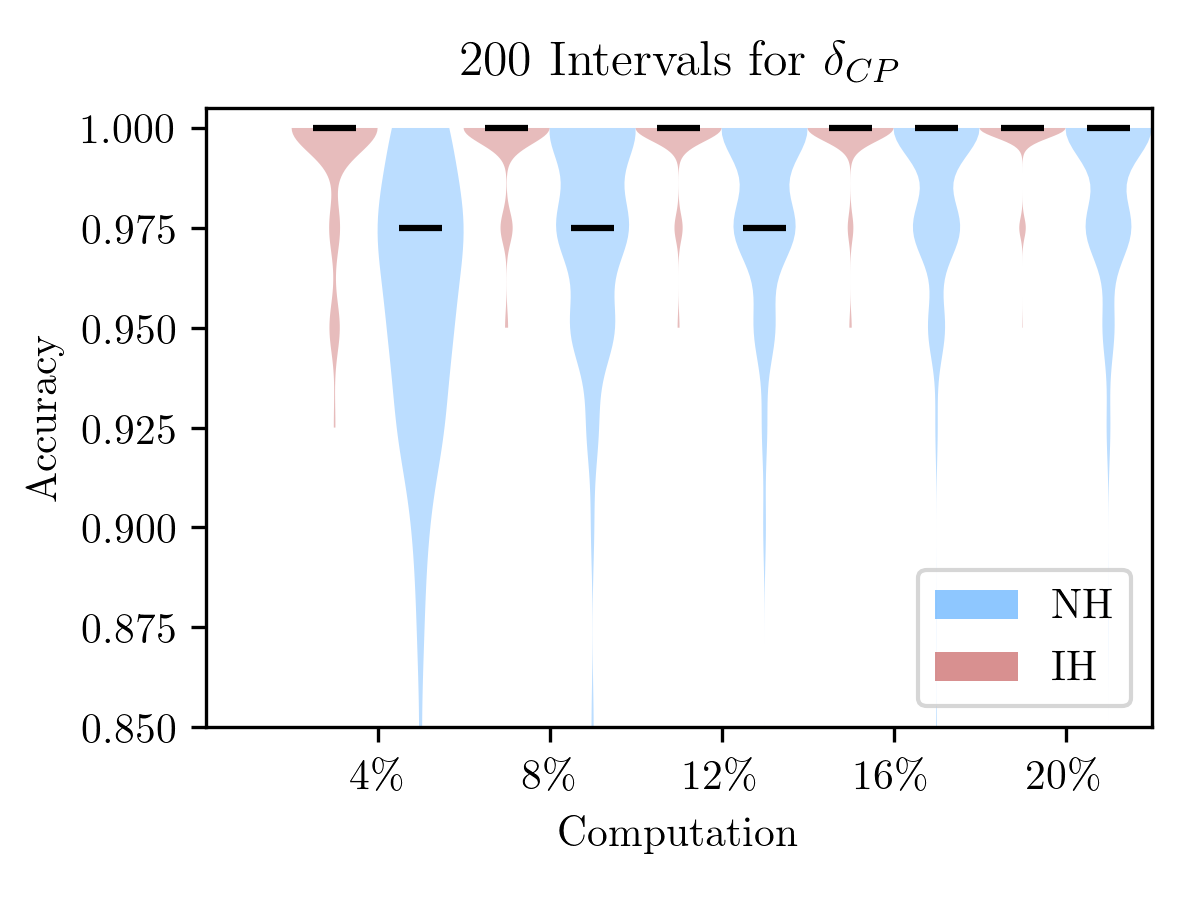
\includegraphics[scale=0.6]{figures_final/compare_interval.png}}
  \end{columns}
  \begin{itemize}
    \item Median Accuracies for 1D is 100\%, for 2D is $> 99.5\%$ (both NH, IH)
    \item Mean Accuracies for 1D is 98.5\% (99.8\%) for NH (IH), for 2D is $> 99\%$ (both NH, IH)
  \end{itemize}
\end{frame}

\begin{frame}
  \frametitle{Summary and Conclusions}
  \begin{itemize}
    \item Neutrino oscillation experiments provide interesting test case for estimating frequentist confidence intervals
    \item LBL experiments typically proceed via Feldman-Cousins
    \item However, simulating LRT distributions across multi-dimensional parameter space requires huge computational resources
    \item We've studied a Bayesian approach using Gaussian processes on a toy LBL set-up
    \item Helps us estimate frequentist contour edges to quite a high accuracy without having to sample the entire parameter space!
    \item Order of magnitude gain in computation!
    \item All code with illustrative notebooks here : \url{https://github.com/nitish-nayak/ToyNuOscCI}, maintained by Lingge (linggeli7@gmail.com) and myself (nayakb@uci.edu)
  \end{itemize}
\end{frame}

\setbeamertemplate{section page}[mine]
\section{Backup}

\begin{frame}
  \frametitle{$\mathcal{GP}$ Technical Details}
  \begin{itemize}
    \item Rasmussen and Williams has a good discussion about convergence to true functions in regression settings (typically using squared loss functions) : \url{http://www.gaussianprocess.org/gpml/chapters/RW7.pdf}
    \item Well behaved $\implies$ expressible as a generalised fourier series of kernel eigenfunctions
    \item If kernel is non-degenerate, approximation is guaranteed to converge to true function 
    \item If degenerate, convergence towards an $L_{2}$ approximation of the true function
    \item Rates of convergence typically depends on mean and kernel smoothness as well as smoothness of the true function
  \end{itemize}
\end{frame}

\begin{frame}
  \frametitle{$\mathcal{GP}$ Fitting}
  \begin{itemize}
    \item Hyperparameters (\textbf{w}) learned via maximising log marginal likelihood : 
      \begin{equation*}
        p(\textbf{y} | \textbf{X}, \textbf{w}) = \int p(\textbf{y} | \textbf{X}, \textbf{w}, \textbf{f})p(\textbf{f} | \textbf{X}, \textbf{w}) d\textbf{f}
      \end{equation*}
    \item Clearly,
      \begin{equation*}
        \textbf{f} | \textbf{X}, \textbf{w} \sim \mathcal{N}(\textbf{0}, K(\textbf{X}, \textbf{w}))
      \end{equation*}
    \item Some algebra gives us : 
      \begin{equation*}
        -2\log p(\textbf{y} | \textbf{X}, \textbf{w}) = \textbf{y}^{T}K^{-1}\textbf{y} + \log |K| + n\log 2\pi
      \end{equation*}
    \item Minimising above equation gives us a good choice for \textbf{w}
    \item $log |K|$ acts as a penalty term for complexity and therefore reduces overfitting to data
  \end{itemize}
\end{frame}

\begin{frame}
  \frametitle{$\mathcal{GP}$ for FC}
  \begin{itemize}
    \item "Gaussian" not a statement of the underlying distribution of the test statistic, which can still be heavily non-Gaussian
    \item Rather, "Gaussianity" for a stochastic process generating the test statistic distributions. Stochasticity mostly from finite FC grid resolution or finite number of MC experiments for simulating the test statistic distribution 
    \item Assumption we're making for this stochasticity is that it can be parameterised by a kernel describing the relationship between the distributions at neighbouring points $\implies$ multi-variate gaussian
      \bigskip
    \item Also important to note, no real statement about FC coverage or handling of nuisance parameters. Assumes FC gives desired level of coverage
    \item Confidence Intervals still with frequentist interpretation
    \item Bayesian interpretation for "classification probability" of points in parameter space for desired confidence regions
    \item A good summary would be "Accelerating Frequentist CI search by estimating CI edges through Bayesian ML"
  \end{itemize}
\end{frame}

\begin{frame}
\frametitle{Pseudo-code}
\begin{algorithm}[H]
  \caption{$\mathcal{GP}$ iterative confidence contour finding}
  \begin{algorithmic}
    \For{each iteration $t = 1,2,...$}
    \State Propose new points in parameter space $\argmax_\theta a(\theta)$
    \For{each point $\theta'$}
    \State Simulate likelihood ratio distribution
    \For{$k = 1,2,...$}
    \State Perform a pseudo experiment
    \State Maximize the likelihood with respect to $(\theta, \delta)$
    \State Maximize the likelihood with constraint $\theta=\theta'$
    \EndFor
    \State Obtain critical value $c(\theta')$
    \EndFor
    \State Update $\mathcal{GP}$ approximation $\hat{c}(\theta)$
    \State Update confidence contours
    \EndFor
  \end{algorithmic}
\end{algorithm}
\end{frame}

\begin{frame}
  \frametitle{Results : NH, $sin^{2}\theta_{23}-\delta_{CP}$}
  \begin{columns}
    \column{0.5\textwidth}
    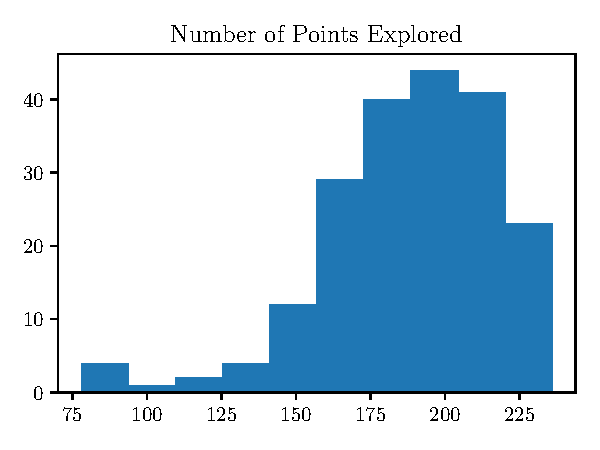
\includegraphics[scale=0.6]{figures_final/points.pdf}
    \column{0.5\textwidth}
    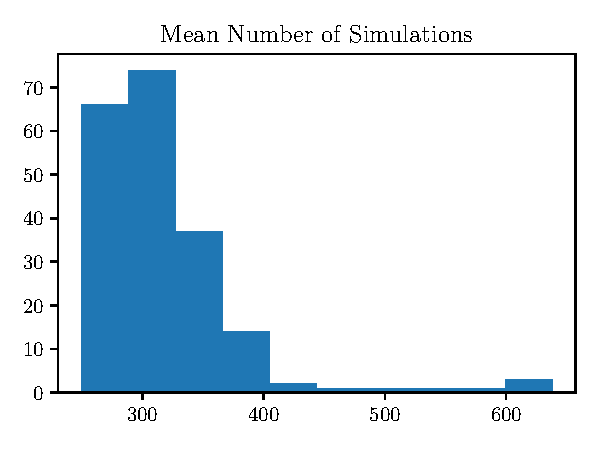
\includegraphics[scale=0.6]{figures_final/sample.pdf}
  \end{columns}
\end{frame}

\begin{frame}
  \frametitle{NH, $sin^{2}\theta_{23}-\delta_{CP}$}
  \centering
  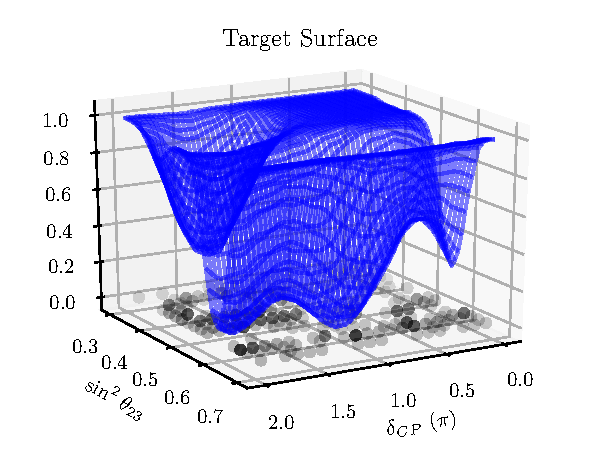
\includegraphics[scale=0.75]{figures_final/target_sdcp.pdf}
\end{frame}

\begin{frame}
  \frametitle{NH, $sin^{2}\theta_{23}-\delta_{CP}$}
  \centering
  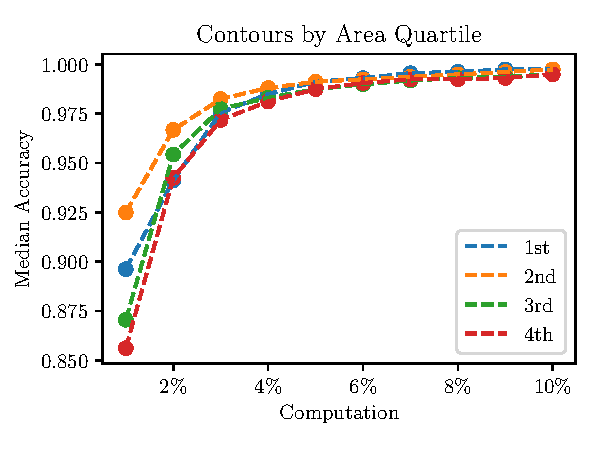
\includegraphics[scale=0.75]{figures_final/compare_area_sdcp.pdf}
\end{frame}

\begin{frame}
  \frametitle{NH, $sin^{2}\theta_{23}-\Delta m^{2}_{32}$}
  \centering
  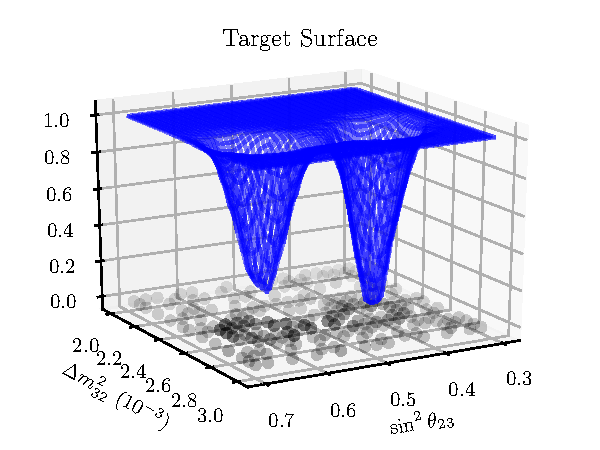
\includegraphics[scale=0.75]{figures_final/target.pdf}
\end{frame}

\begin{frame}
  \frametitle{NH, $sin^{2}\theta_{23}-\Delta m^{2}_{32}$}
  \centering
  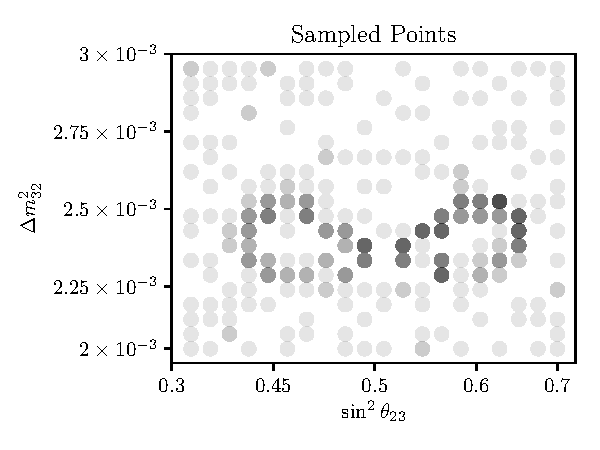
\includegraphics[scale=0.75]{figures_final/sample_2d.pdf}
\end{frame}
\begin{frame}
  \frametitle{NH, $sin^{2}\theta_{23}-\Delta m^{2}_{32}$}
  \centering
  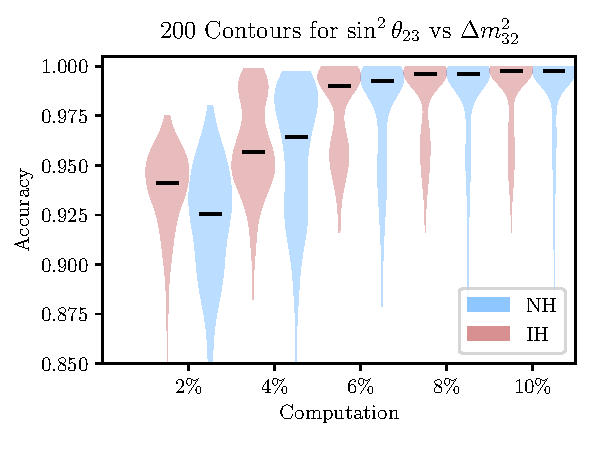
\includegraphics[scale=0.75]{figures_final/compare_contour.pdf}
\end{frame}
\end{document}
